\documentclass[11pt,a4paper]{article}

\usepackage[utf8]{inputenc}
\usepackage[english]{babel}
\usepackage[left=2cm,right=2cm,top=2cm,bottom=2cm]{geometry}

\usepackage{csquotes}
\usepackage{graphicx}
\graphicspath{ {./figs} }
\usepackage{float}
\usepackage{wrapfig}

\usepackage{caption}
\usepackage{subcaption}

\usepackage{amsmath}
\usepackage{amssymb}
\usepackage{amsthm}

\usepackage{mathrsfs}
\usepackage{mathtools}

\usepackage{color}
\usepackage{epsfig}
\usepackage{array}
\usepackage{multicol}
\usepackage{tikz}
\usepackage{listings}
\usepackage{minted}
\usepackage{mdframed}

\setlength{\parindent}{0em}
\setlength{\parskip}{0.5em}
% \textwidth 6.5in
% \textheight 9.in
% \oddsidemargin 0in
% \headheight 0in


\newtheorem{theorem}{Theorem}[section]

\definecolor{codegreen}{rgb}{0,0.6,0}
\definecolor{codegray}{rgb}{0.5,0.5,0.5}
\definecolor{backcolour}{rgb}{0.95,0.95,0.95}

\usepackage[hidelinks]{hyperref}
\hypersetup{
    colorlinks=false, %set true if you want colored links
    linktoc=all,      %set to all if you want both sections & subsections linked
}
\usepackage[nameinlink]{cleveref}


\lstset{ %
  language=python,                % choose the language of the code
  basicstyle=\footnotesize,       % the size of the fonts that are used for the code
  numbers=left,                   % where to put the line-numbers
  numberstyle=\footnotesize,      % the size of the fonts that are used for the line-numbers
  stepnumber=1,                   % the step between two line-numbers. If it is 1 each line will be numbered
  numbersep=5pt,                  % how far the line-numbers are from the code
  backgroundcolor=\color{white},  % choose the background color. You must add \usepackage{color}
  showspaces=false,               % show spaces adding particular underscores
  showstringspaces=false,         % underline spaces within strings
  showtabs=false,                 % show tabs within strings adding particular underscores
  frame=single,                   % adds a frame around the code
  tabsize=2,                      % sets default tabsize to 2 spaces
  captionpos=b,                   % sets the caption-position to bottom
  breaklines=true,                % sets automatic line breaking
  breakatwhitespace=false,        % sets if automatic breaks should only happen at whitespace
  escapeinside={\%*}{*)}          % if you want to add a comment within your code
}

\usemintedstyle{vs}


\begin{document}


\usetikzlibrary{positioning}
\tikzset{every picture/.style={line width=0.75pt}}

\pagestyle{plain}

\begin{multicols}{2}
  \begin{flushleft}
    MAT360 \\
    Autumn 2021\\
    Prof. Jan Martin Nordbotten\\
    \underline{University of Bergen}
  \end{flushleft}
  \vfill\null
  \columnbreak

  \begin{flushright}
    
\includegraphics[height=2cm]{assets/uib.logo.png}
  \end{flushright}
\end{multicols}

\begin{center}
\textbf{\large Exemplary FEM implementations and convergence analysis}\\
Paul Stryck\\
\end{center}
\rule{\linewidth}{0.1mm}



\begin{abstract}
    \noindent
    This report presents the numerical validation of a custom FEM implementation with polynomial basis
    functions of arbitrary degree on structured and unstructured grids.
    The Poisson equation will be considered on the unit square.
    Different force functions for which the analytical solution is known will be used.
    Thus, the errors can be computed explicitly, and given convergence rates are verified.
    To cover a broad spectrum of potential implementation errors, both pure Dirichlet and mixed Dirichlet +
    Neumann boundary conditions will be used.
\end{abstract}

\begin{multicols}{2}

\subsection*{Continuous Problem}
The PDE under consideration is the homogeneous Poisson equation:
\begin{equation} \label{eq:poisson}
  \begin{split}
    - \Delta u &= f \quad \text{on } \Omega\\
    u &= 0 \quad \text{on } \partial\Omega
  \end{split}
\end{equation}
Where $\Omega \subset \mathbb{R}^n$ is an open and bounded set and $f \in L^2(\Omega)$.
A classical solution $u \in C^2(\Omega) \cap C^1(\bar{\Omega})$, will at most
exist if $f$ is at least continuous and restrictive assumptions regarding $\Omega$ have to be made.
Thus, a less restrictive formulation of the Problem (\ref{eq:poisson}) based on
the variational formulation will be derived.\\

Multiplying \autoref{eq:poisson} with test functions $v \in C^\infty_0(\Omega)$ and
integrating over $\Omega$ yields:

\begin{equation} \label{eq:poisson_var}
    - \int_\Omega \Delta u v\,dV = \int_\Omega fv\,dV \\ \forall v \in C^\infty_0(\Omega)
\end{equation}

If $\Omega$ has a Lipschitz boundary, \autoref{eq:poisson_var} can be simplified
using Green's first identity.
\begin{multline}\label{eq:poisson_var_greens}
    \int_\Omega \nabla u \cdot \nabla v \,dV
  - \int_{\partial\Omega} v \frac{\partial u}{\partial n} \,dS
  = \int_\Omega fv\,dV \\ \forall v \in C^\infty_0(\Omega)
\end{multline}

Where the boundary integral vanishes since $v = 0$ on $\partial\Omega$.
Additionally, $C^\infty_0(\Omega)$ is dense in $H^1_0(\Omega)$.
So \autoref{eq:poisson_var_greens} can be further simplified to:
\begin{equation} \label{eq:poisson_weak}
  \underbrace{\int_\Omega \nabla u \cdot \nabla v \,dV}_{\eqqcolon a(u,v)}
  = \underbrace{\int_\Omega fv\,dV \quad \forall v \in
  H^1_0(\Omega)}_{\eqqcolon b(v) = \langle b, v \rangle_{H^{-1}_0, H^1_0}}
\end{equation}
A function $u \in H^1_0(\Omega)$ satisfying \autoref{eq:poisson_weak} is called
weak solution of \autoref{eq:poisson}.
Assuming $u \in C^2(\Omega) \cap C^1(\bar{\Omega})$ is a classical solution to
\autoref{eq:poisson}. This implies $u \in H^1_0(\Omega)$ and thus any classical
solution would also satisfy the weak formulation. Thus, the weak formulation
indeed broadens the set of admissible functions.

Existence and uniqueness of a solution to \autoref{eq:poisson_weak} is given by
reformulating \autoref{eq:poisson_weak} to $a(u,v) = \langle b,v \rangle_{H^{-1}_0, H^1_0}$
and application of Lax-Milgram. The proof is omitted here.


\subsection*{Boundary Conditions}
It shall be briefly investigated how boundary conditions can be incorporated.
For this, Dirichlet and mixed Dirichlet + Neumann boundary conditions will be
considered.\\
First, considering Dirichlet boundary conditions, the problem is given by:
\begin{equation} \label{eq:poisson_dirichlet}
  \begin{split}
    -\Delta u &= f  \text{ in } \Omega\\
    u &= g \text{ on } \partial\Omega
  \end{split}
\end{equation}
with $f \in L^2(\Omega)$ and $g \in L^2(\partial\Omega)$.\\
In addition to the already established Hilbert space $H^1_0$ define the set:
\begin{equation*}
    V_g \coloneqq \left\{ v \in H^1(\Omega)\, :\, v\vert_{\partial\Omega} = g \text{ a.e. on } \partial\Omega\right\}
\end{equation*}
Which is well-defined for all $g \in L^2(\partial\Omega)$ by the trace
theorem. $H^1_0$ is of course a Hilbert space, whereas $V_g$ is not since it is
not closed under addition.

By using test functions from $H^1_0(\Omega)$, the weak formulation stays the
same as in \autoref{eq:poisson_weak} however, with solutions $u$ sought in $V_g$.
To obtain such a solution: Define the bilinear form $a$ and linear
functional $b$ as before:
\begin{equation*}
  \begin{split}
    a(u,v) &= \int_\Omega \nabla u \cdot \nabla v \,dx\\
    b(v)   &= \int_\Omega fv\,dx
  \end{split}
\end{equation*}

Now choose an arbitrary $\hat{g}\in V_g$ and solve:
\begin{equation*}
  a(\hat{u},v) = b(v) - a(\hat{g},v) \quad \forall v \in H^1_0(\Omega)
\end{equation*}
Where the existence of a unique solution $\hat{u}$ is guaranteed by Lax-Milgram.

The weak solution to \autoref{eq:poisson_dirichlet} is obtained by:
$$u = \hat{u} + \hat{g} \in V_g$$

\subsubsection*{Neumann Boundary Conditions}
To incorporate Neumann boundary conditions the boundary $\partial\Omega$ needs
to be disjointly split into $\Gamma_0$ and $\Gamma_1$, such that
$\Gamma_0 \cup \Gamma_1 = \partial\Omega$ and $\Gamma_0 \cap \Gamma_1 = \emptyset$.
The Poisson equation with mixed Neumann and homogeneous Dirichlet boundary
conditions can then be stated as:
\begin{equation} \label{eq:poisson_neumann}
  \begin{split}
    -\Delta u &= f  \text{ in } \Omega \\
    u &= 0 \text{ on } \Gamma_0 \\
    \frac{\partial u}{\partial n} &= h \text{ on } \Gamma_1, \quad h\in L^2(\Gamma_1)
  \end{split}
\end{equation}

The weak formulation of \autoref{eq:poisson_neumann} is given by:
\begin{multline}
  \int_\Omega \nabla u \cdot \nabla v\,dx
  = \int_\Omega fv\,dx + \int_{\Gamma_1}hv\,dx \\
  \forall v \in \left\{ v \in H^1(\Omega)\, :\, v\vert_{\Gamma_0} = 0 \text{ a.e. on } \Gamma_0\right\}
\end{multline}

By application of Lax-Milgram, it can be verified that \autoref{eq:poisson_neumann}
admits a unique, weak solution if $\int_{\Gamma_0}1\,dx > 0$.
In the case of pure Neumann conditions Lax-Milgram cannot be applied, since the
bilinear form is no longer coercive and solutions are only unique up to a constant.
To extend this to the case of $u = g$ on $\Gamma_0$ for some $g \in L^2(\Gamma_0)$
the same idea used for pure Dirichlet boundary conditions can be used.

\subsection*{Discretizing the Problem}
To obtain numerical solutions to \autoref{eq:poisson_weak}, the problem has to be
discretized. As by the lecture, the Hilbert space $H^1(\Omega)$ can be
successively approximated by some sequence of finite dimensional subspaces
$(V_i)_{i\in \mathbb{N}}$.\\
For now, the $V_i$ will be the space of piecewise linear, continuous
polynomials defined on a set of nodes obtain by a triangulation of $\Omega$.
Under the assumption that the triangulation is conforming and no triangles
collapse, it has been shown in the lecture that $\lim\limits_{i\to\infty}V_i \to
H^1(\Omega)$.

By forcing all basis functions to attain a certain value on the boundary, an
approximation to the set $V_g$ can be obtained. By forcing them to 0 on the
boundary, the space $H^1_0(\Omega)$ can be obtained and
$\lim\limits_{i\to\infty}V_i \to H^1_0(\Omega)$

Thus, the continuous problem $a(u,v) = b(v) \quad \forall v \in H^1_0(\Omega)$
can be approximated by the finite dimensional problem $a(u_i,v_i) = b(v_i)$ for all
basis vectors $v_i \in V_i$ (and explicitly enforcing the 0 boundary condition).

Since there are only a finite number of basis functions, this results in a linear system
where the properties of the system heavily depend on the choice of basis of $V_i$.

In this work, isoparametric Lagrange elements are chosen as a basis,
which results in a sparse system.

\section*{Numerical Validation with 1\textsuperscript{st} Order Piecewise Polynomials}
Different convergence rates, shown in the lecture are given by:
\begin{equation}
  \begin{split}
    \left|u-u_h\right|_{H^1(\Omega)} &\lesssim h \lVert u\rVert^2_{H^2(\Omega)}\\
    \lVert u - u_h \rVert_{L^2(\Omega)} &\lesssim h\lVert u\rVert^2_{H^1(\Omega)}\\
    \lVert u - u_h \rVert_{L^2(\Omega)} &\lesssim h^2\lVert u\rVert^2_{H^2(\Omega)}
  \end{split}
\end{equation}
Where $h$ is depended on the grid and $u \in H^2(\Omega)$ or $u \in H^1(\Omega)$
is the analytical solution to $a(u,v) = b(v)$.
$u_h$ is the solution to the discretized problem.

\subsection*{Smooth Solutions $u \in H^2$}
Throughout this report, all numerical experiments concerned with convergence rely
on a gradually refined grid. Here, $n$ will always denote the number of vertices
per edge on the unit square. Resulting in $n^2$ vertices in total and thus $h \sim \frac{1}{n}$.
How such refinements for structured and unstructured grids works can be seen in \autoref{fig:grids}

\begin{figure}[H]
  \centering
  \begin{subfigure}{.5\linewidth}
    \centering
    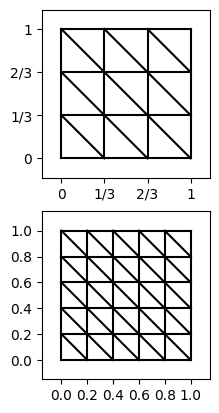
\includegraphics[width=.9\linewidth]{structured_grids}
    \caption{Structured Grids}
  \end{subfigure}%
  \begin{subfigure}{.5\linewidth}
    \centering
    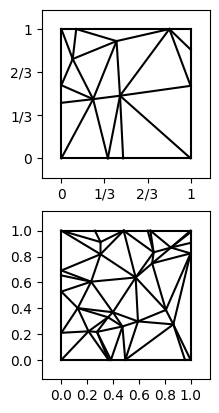
\includegraphics[width=.9\linewidth]{unstructured_grids}
    \caption{Unstructured Grids}
  \end{subfigure}
  \caption{Grid Refinements for $n=4$ and $n=6$}
  \label{fig:grids}
\end{figure}

Considering the following problem:
\begin{equation}
  \label{eq:smooth_poisson_prob}
  \begin{split}
    \Omega &= \left[0,1\right]^2\\
    -\Delta u &= f\\
    u &= 0 \quad \text{on } \partial \Omega\\
  \end{split}
\end{equation}

With given solution
\begin{multline*}
  u(x,y) = 2^{4a} x^a (1-x)^a y^a (1-y)^a \quad a \in \mathbb{N}\\
  u \in H^2(\Omega)\,\forall a > 0
\end{multline*}
and $f$ accordingly.
This solution has the useful property
$$\lVert u \rVert_{H^2(\Omega)} \sim a.$$
This makes it ideal to verify the above convergence rates.

\begin{figure}[H]
  \centering
  \begin{subfigure}{.5\linewidth}
    \centering
    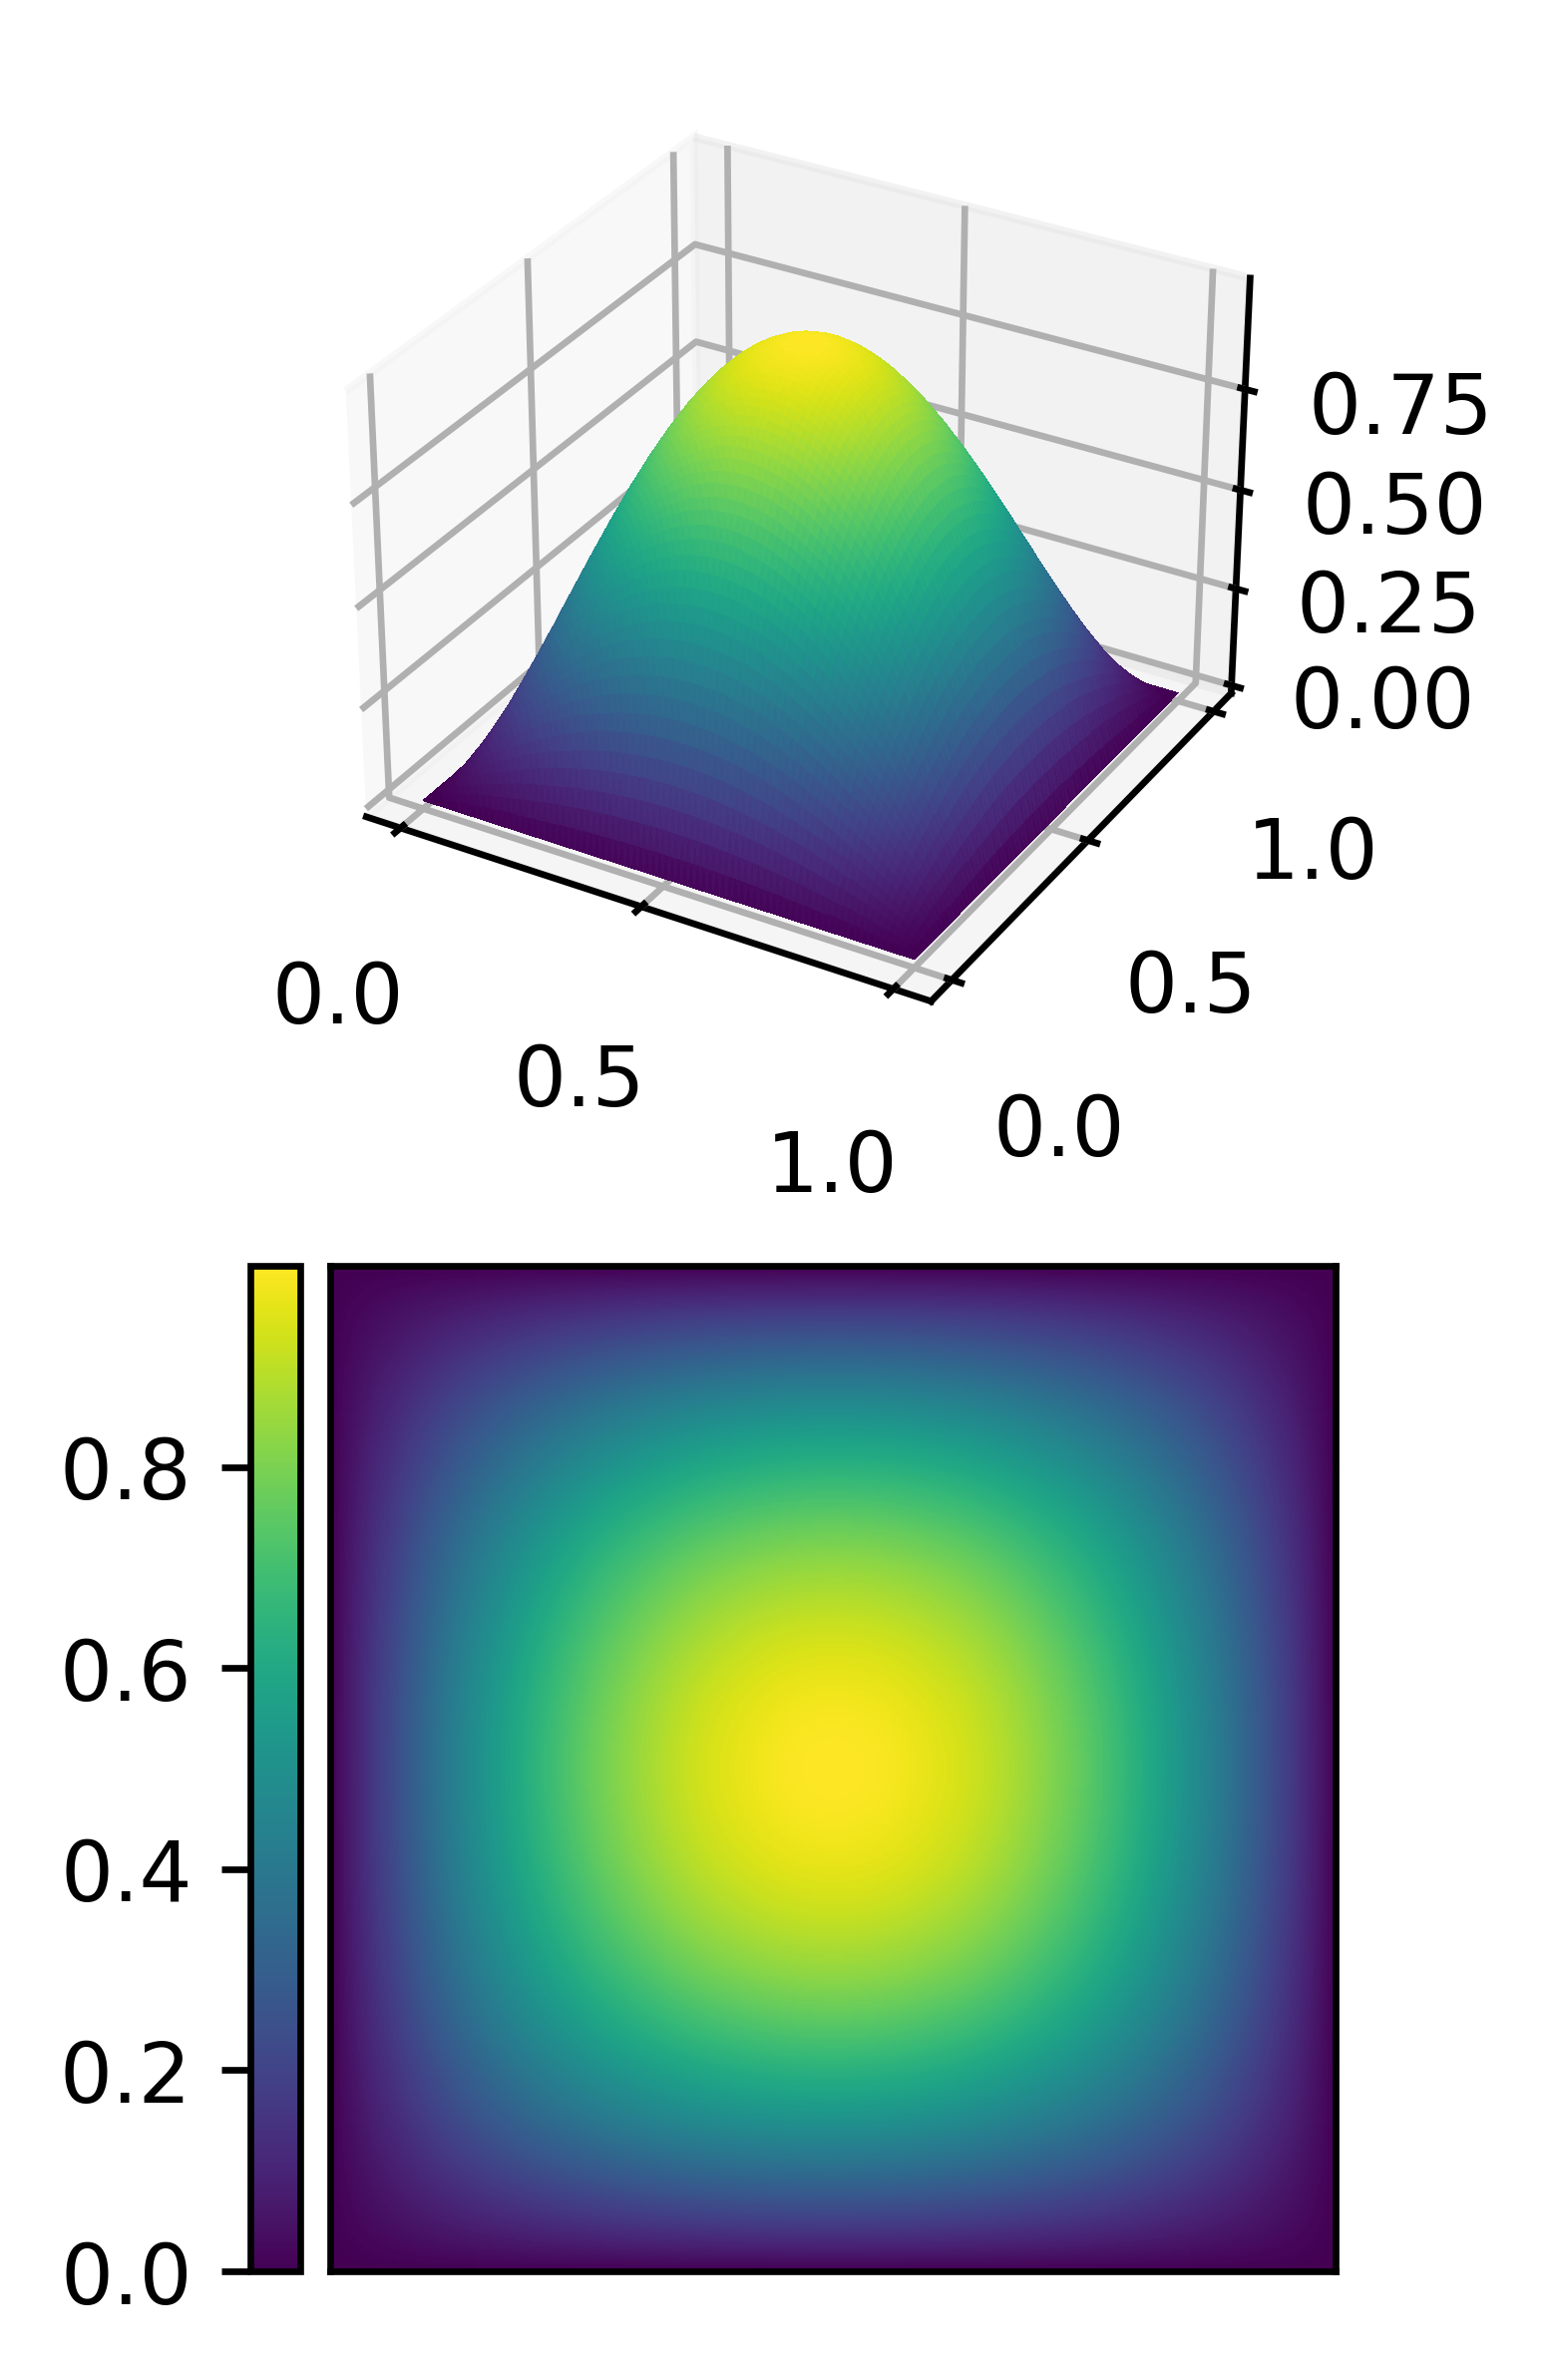
\includegraphics[width=.9\linewidth]{contour_1}
    \caption{$a = 1$}
  \end{subfigure}%
  \begin{subfigure}{.5\linewidth}
    \centering
    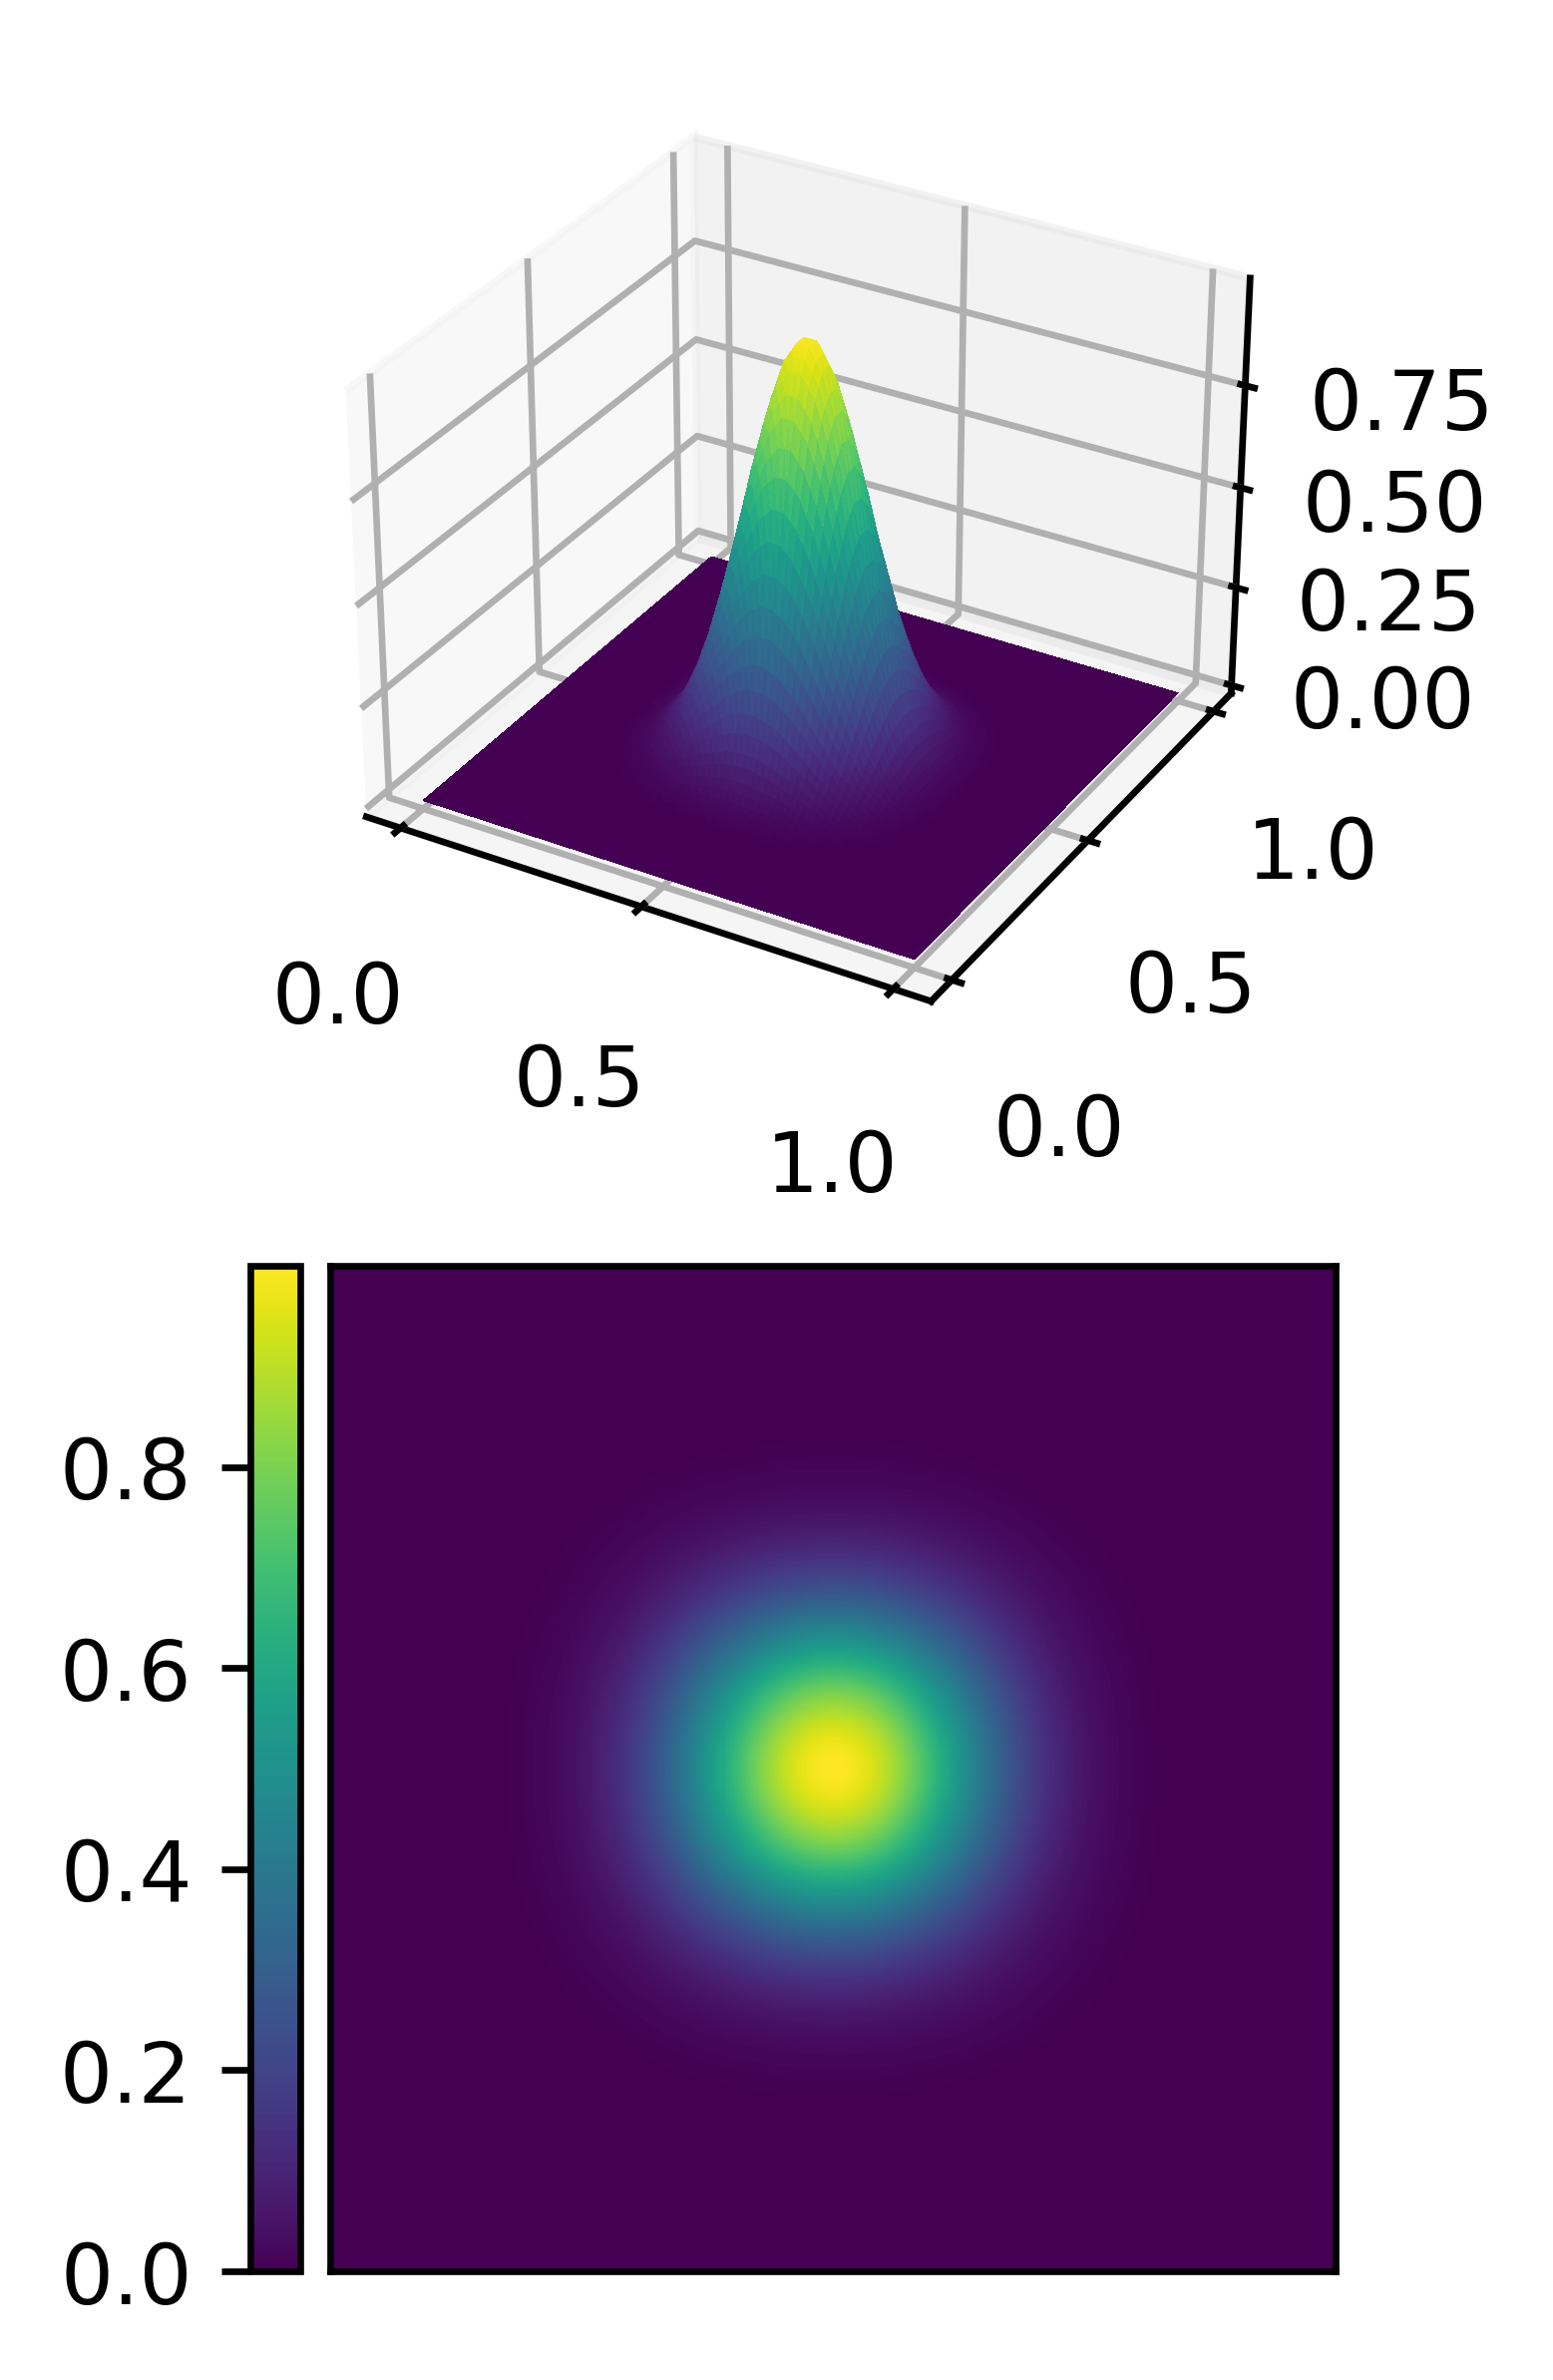
\includegraphics[width=.9\linewidth]{contour_10}
    \caption{$a = 10$}
  \end{subfigure}
  \caption{Solution $u$ with varying parameter $a$}
  \label{fig:smooth_dirichlet_solution}
\end{figure}

As seen in \autoref{fig:smooth_dirichlet_solution}, $u$ is a smooth bump
function where the steepness increases with $a$.
We expect a convergence rate of order $C\cdot h$ for the $H^1$ semi-norm
and $C\cdot h^2$ for the $L^2$ norm since $u \in H^2(\Omega) \forall a > 0$.
C is expected to increase with $a$ as it should stand in some relation to $\lVert u \rVert_{H^2}$.
For both, structured (\ref{fig:smooth_dirichlet_errs_str}) and unstructured (\ref{fig:smooth_dirichlet_errs_unstr})
grids exactly this is observed.

\begin{figure}[H]
  \centering
  \begin{subfigure}{1\linewidth}
    \centering
    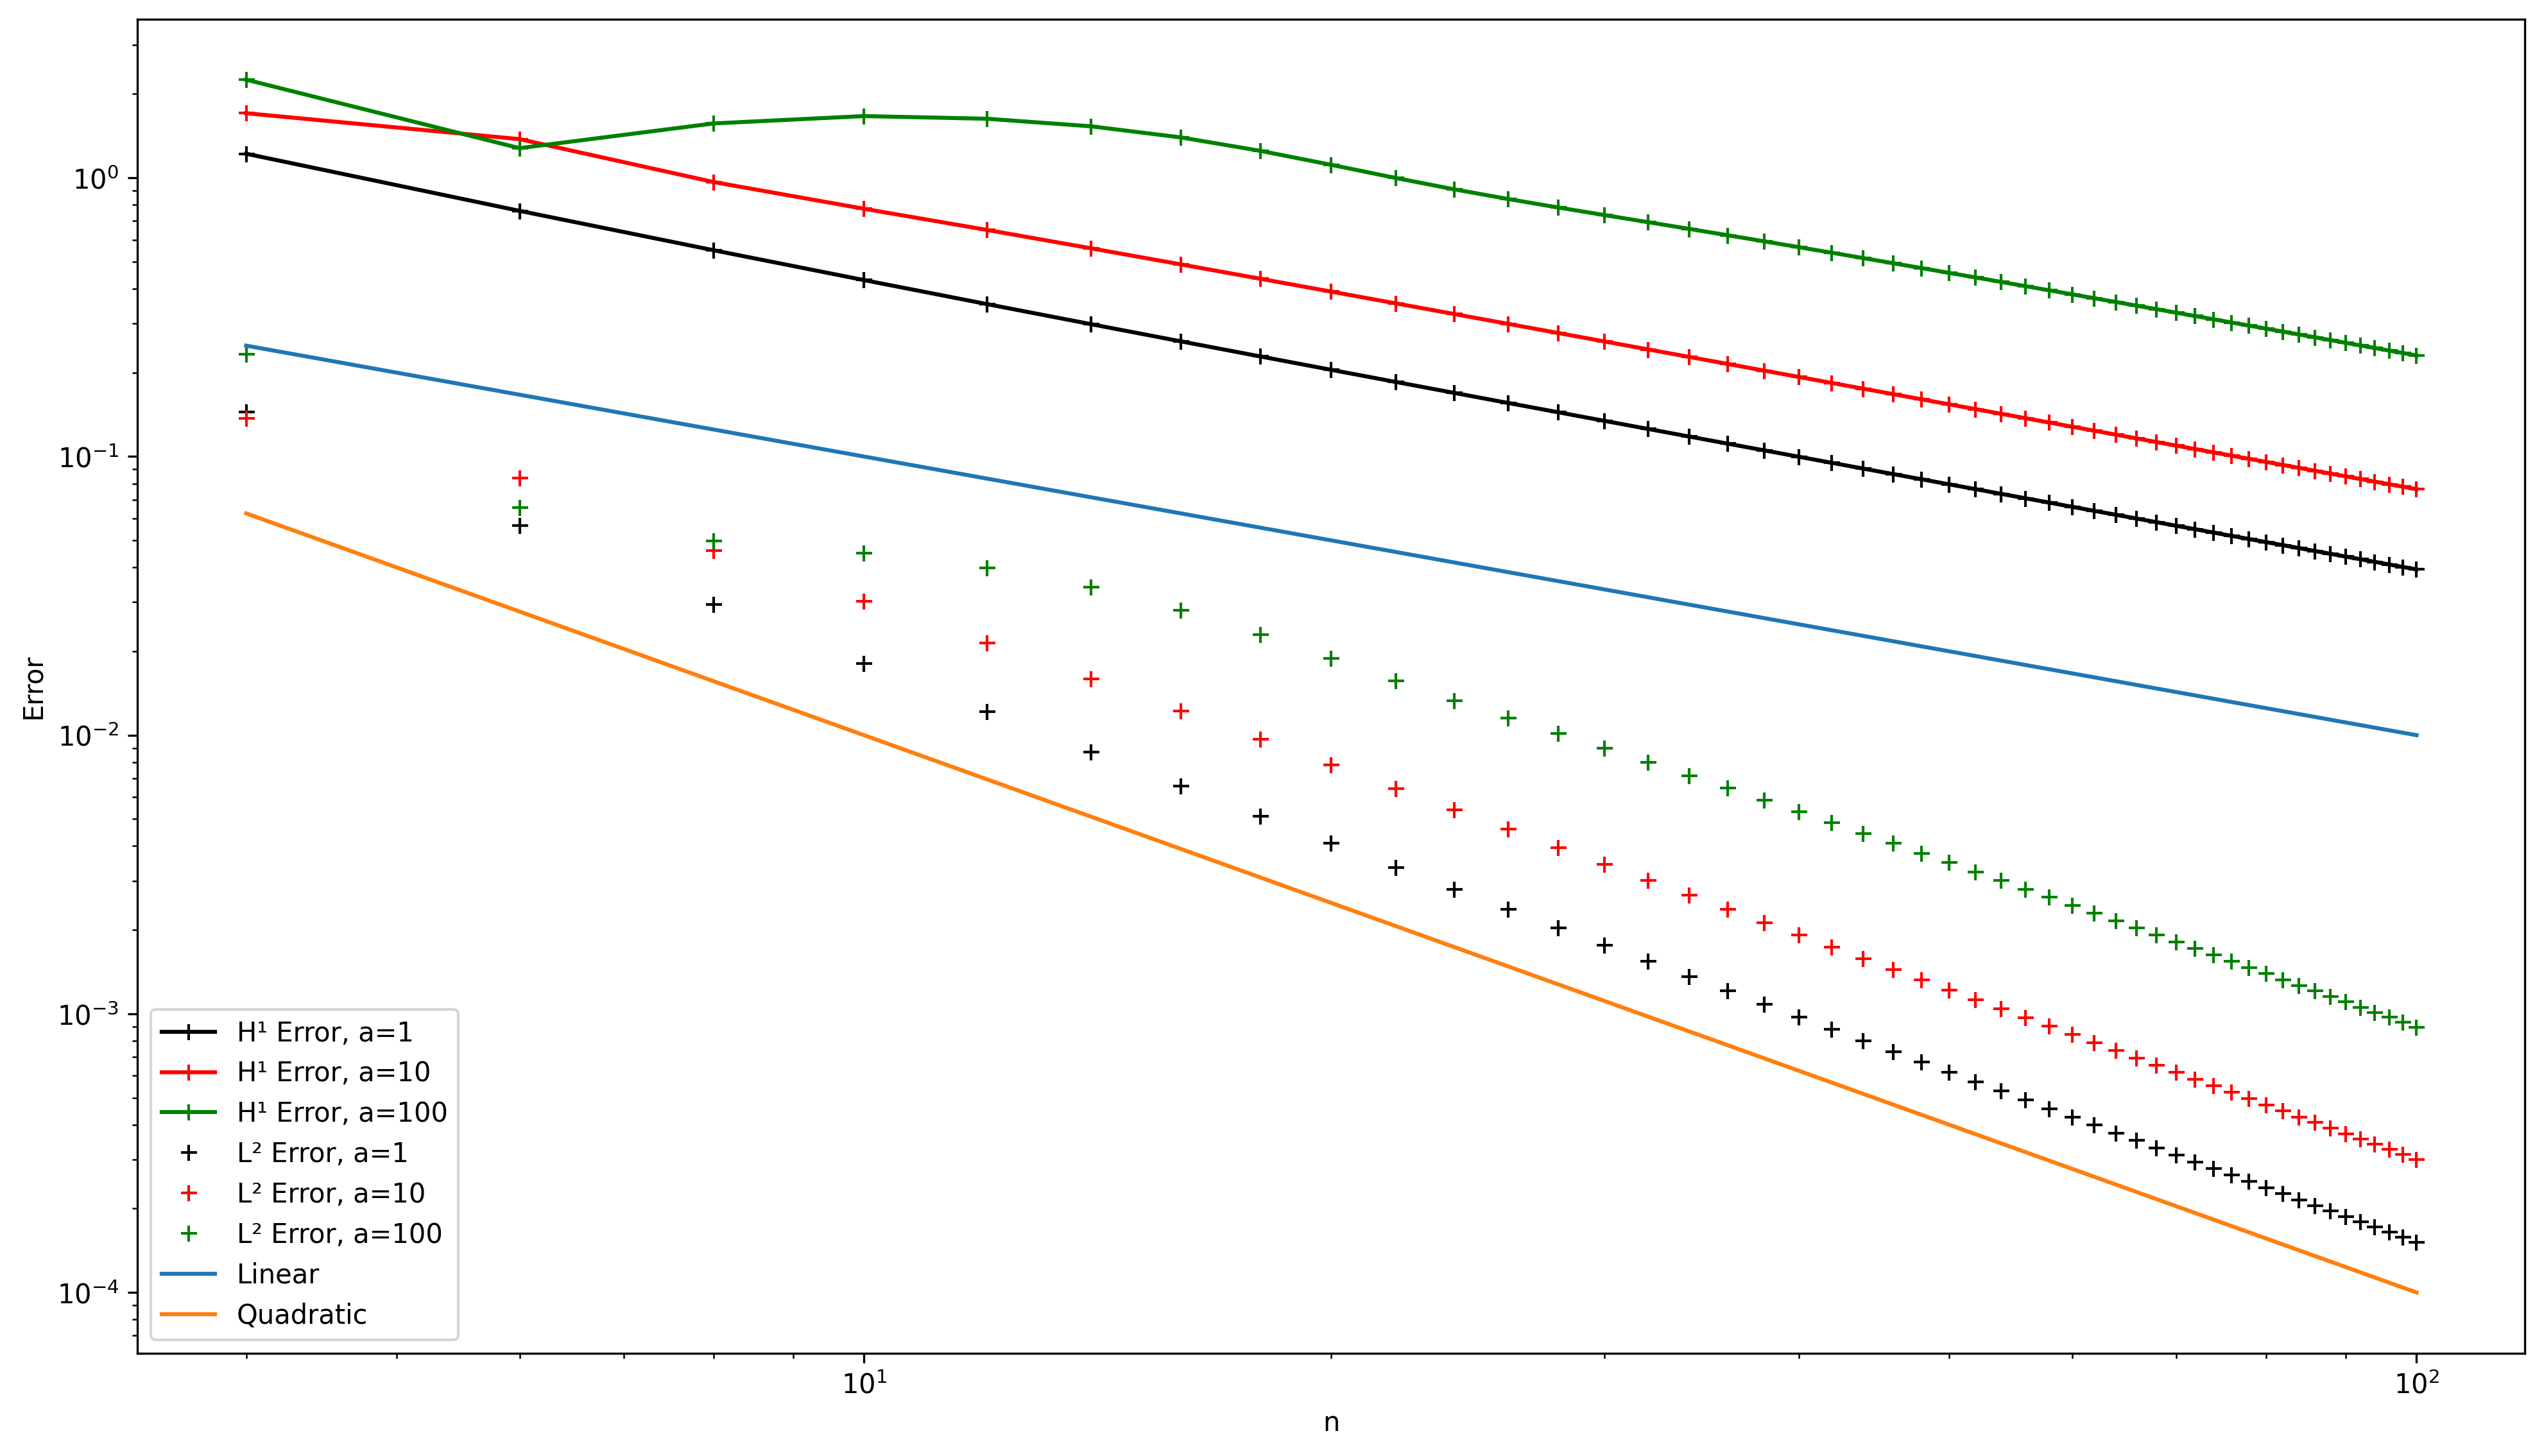
\includegraphics[width=1\linewidth]{errors_smooth_reg}
    \caption{Structured Grids}
    \label{fig:smooth_dirichlet_errs_str}
  \end{subfigure}

  \begin{subfigure}{1\linewidth}
    \centering
    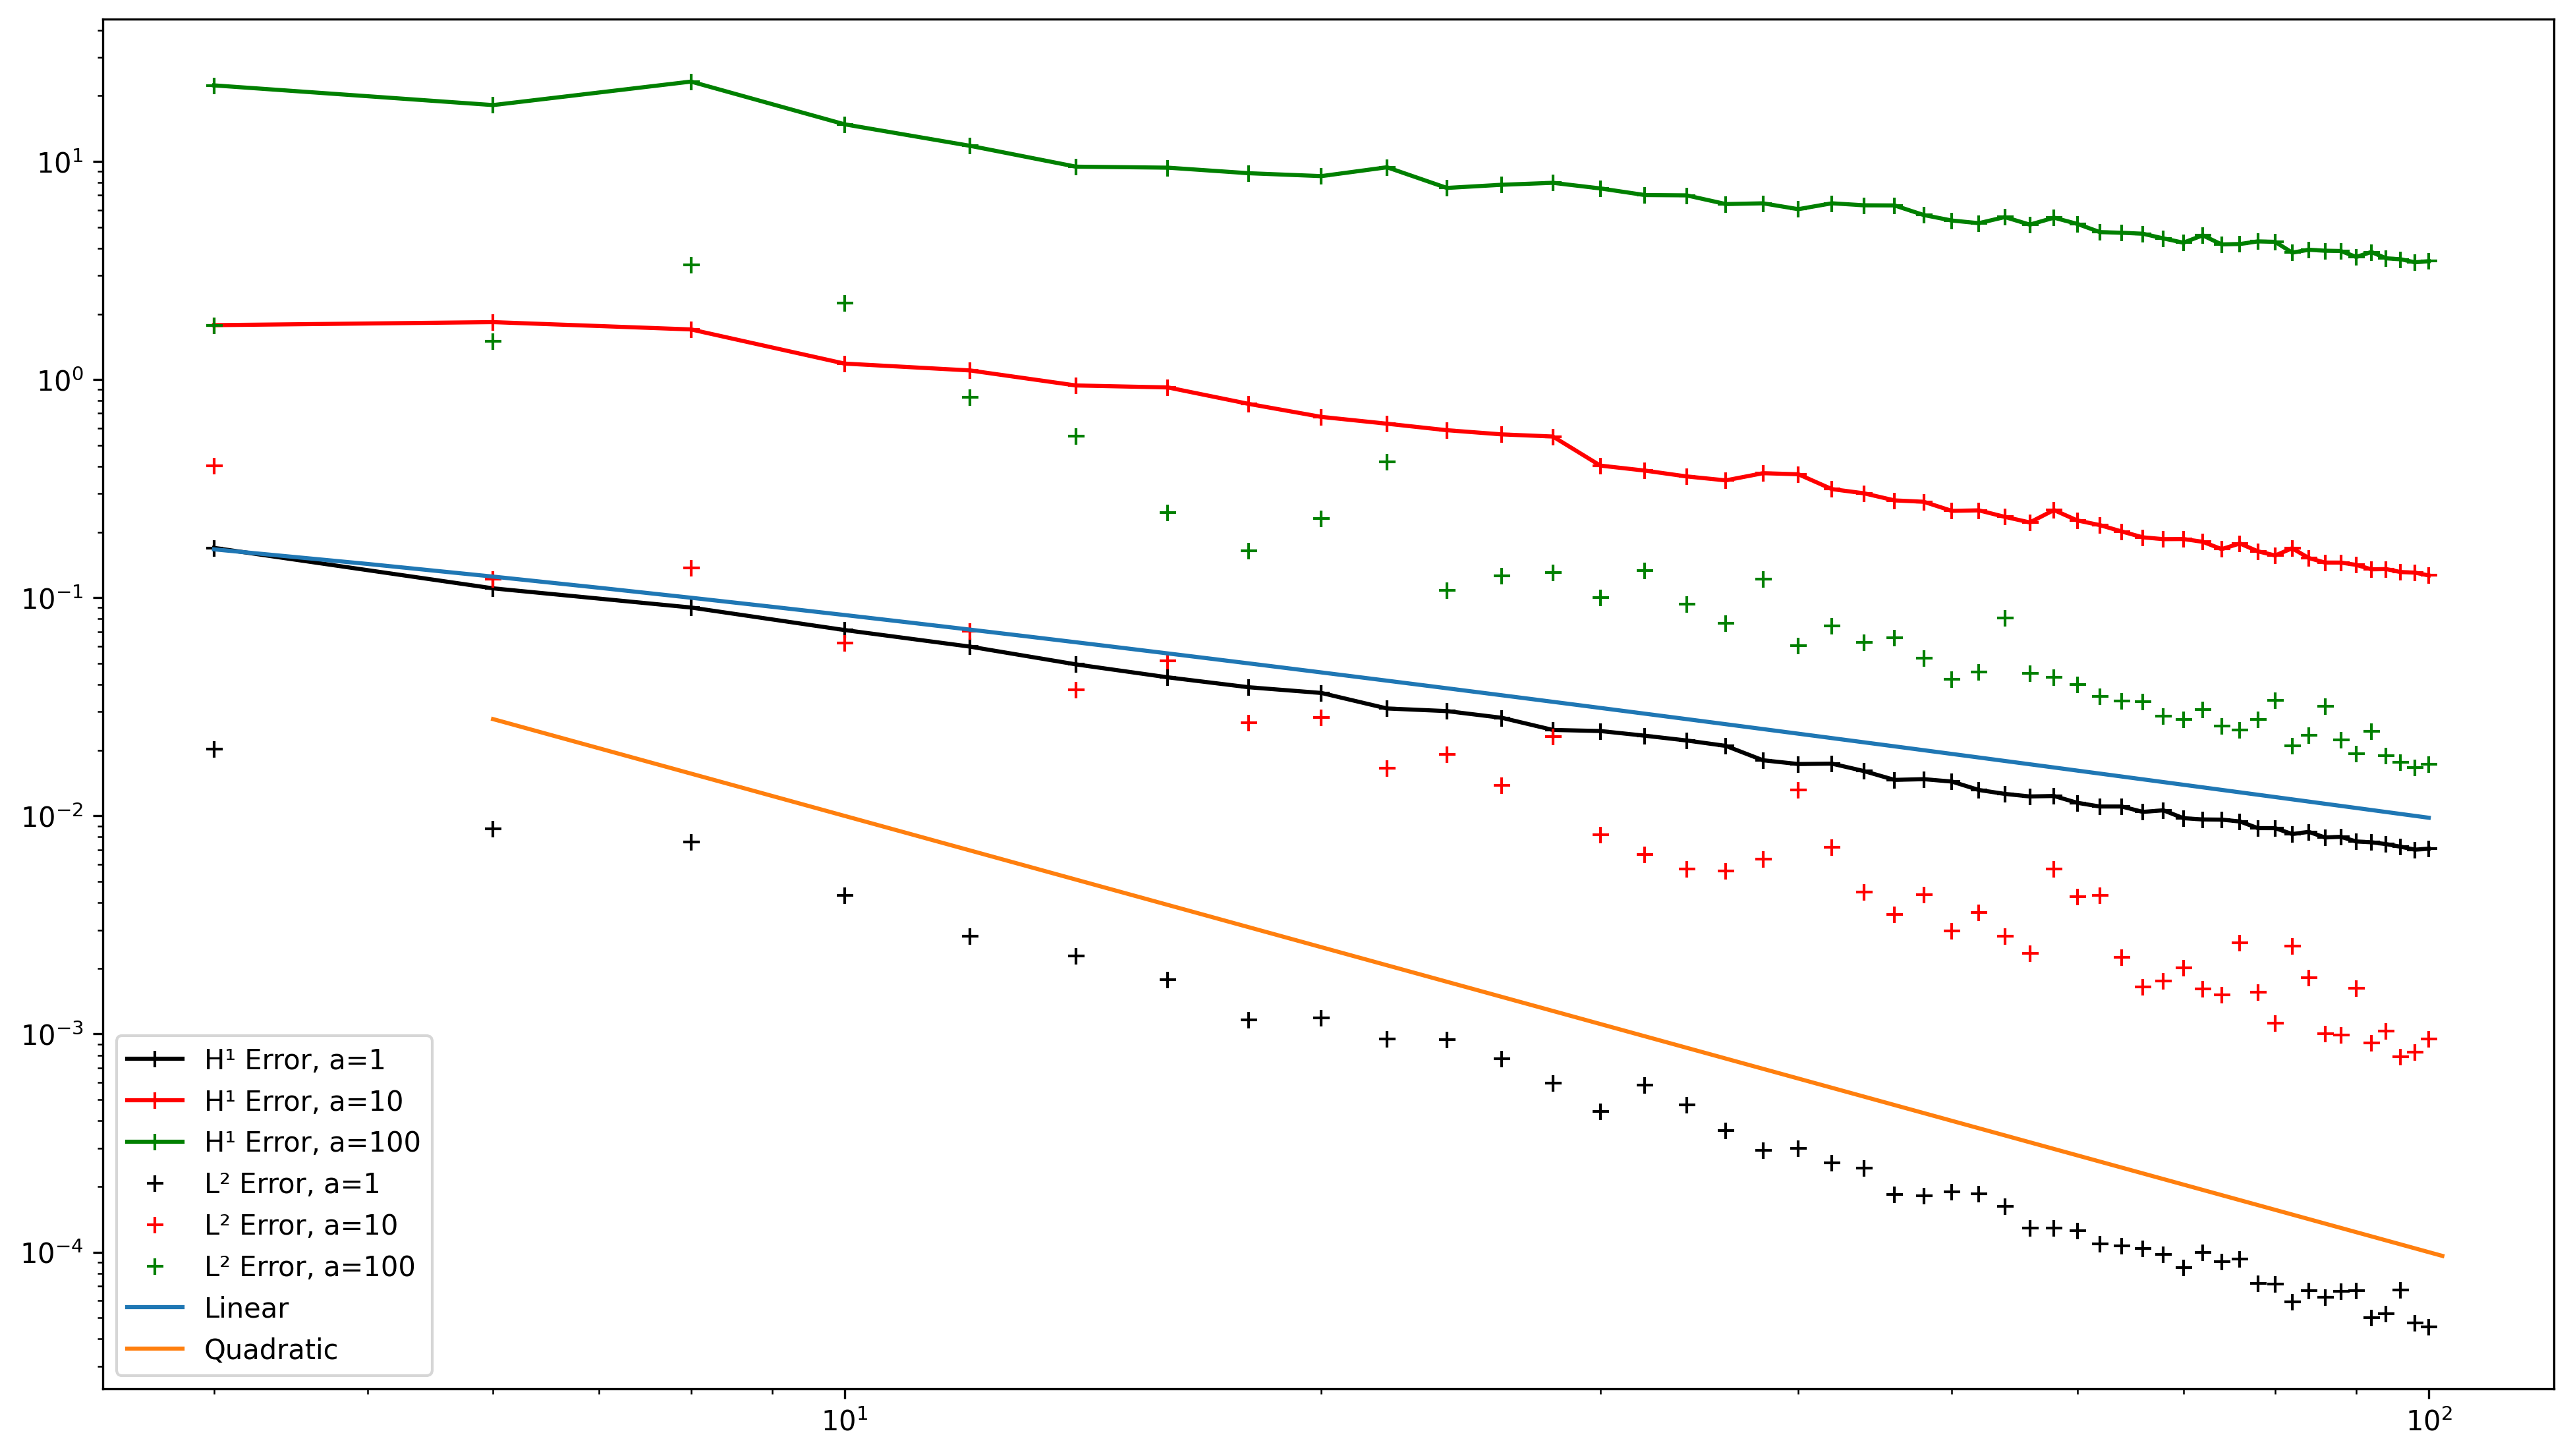
\includegraphics[width=1\linewidth]{errors_smooth_irreg}
    \caption{Unstructured Grids}
    \label{fig:smooth_dirichlet_errs_unstr}
  \end{subfigure}
  \label{fig:smooth_dirichlet_errs}
  \caption{$L^2$ Norm and $H^1$ Semi-Norm Errors for Smooth Solutions on Structured and Unstructured Grids}
\end{figure}

Where the overall error of the solution on the unstructured grid is significantly worse.
This is due to the fact, that no special care has been taken to attain a good quality mesh.


\subsection*{Less Regular Forces}
Considering the following problem with mixed Dirichlet and Neumann boundary conditions.
\begin{equation}
  \label{eq:poisson_less_smooth_prob}
  \begin{split}
    \Omega &= \left[-1,1\right]^2\\
    -\Delta u &= \begin{cases}
      \frac{\pi^2}{4} \operatorname{cos}\left(\frac{\pi}{2} \cdot y\right) \quad &x \le 0\\
      \frac{\pi^2}{4} \operatorname{cos}\left(\frac{\pi}{2} \cdot y\right) - a\left(a-1\right)x^{a-2} \quad &x > 0
    \end{cases}\\
    u(x,y) &= 0 \quad \text{on } [-1,0] \times -1 \cup [-1,0] \times 1\\
    u(x,y) &= x^a \quad \text{on } (0,1] \times -1 \cup (0,1] \times 1\\
    \frac{\partial u}{\partial {\bf n}} &= 0 \quad \text{on } -1 \times (-1,1)\\
    \frac{\partial u}{\partial {\bf n}} &= a \quad \text{on } 1 \times (-1,1)
  \end{split}
\end{equation}
With known solution:
\begin{equation*}
  u(x,y) = \begin{cases}
    \operatorname{cos}\left(\frac{\pi}{2} \cdot y\right) \quad &x \le 0\\
    \operatorname{cos}\left(\frac{\pi}{2} \cdot y\right) + x^a \quad &x > 0
  \end{cases}
\end{equation*}

Where
$$u \in H^{a+0.5 - \epsilon}(\Omega) \quad \forall \epsilon > 0.$$
With increasing $a$, the function $\Delta u$ will develop a singularity along the $x = 0$ line.
\begin{equation}
  \begin{split}
    a \le 1: \quad &u \notin C^0(\Omega)\\
    1 < a \le 1.5: \quad &u \in H^1(\Omega), u \notin H^2(\Omega) \\
    1.5 < a: \quad &u\in H^2(\Omega)
  \end{split}
\end{equation}
$a > 1$ is needed, so the interpolation operator is well-defined, and our established
convergence estimates make sense.
The varying regularity of the boundary conditions does not pose a problem, since only
square integrability for both, the Neumann, and Dirichlet Boundary is needed.

\begin{figure}[H]
  \centering
  \begin{subfigure}{.5\linewidth}
    \centering
    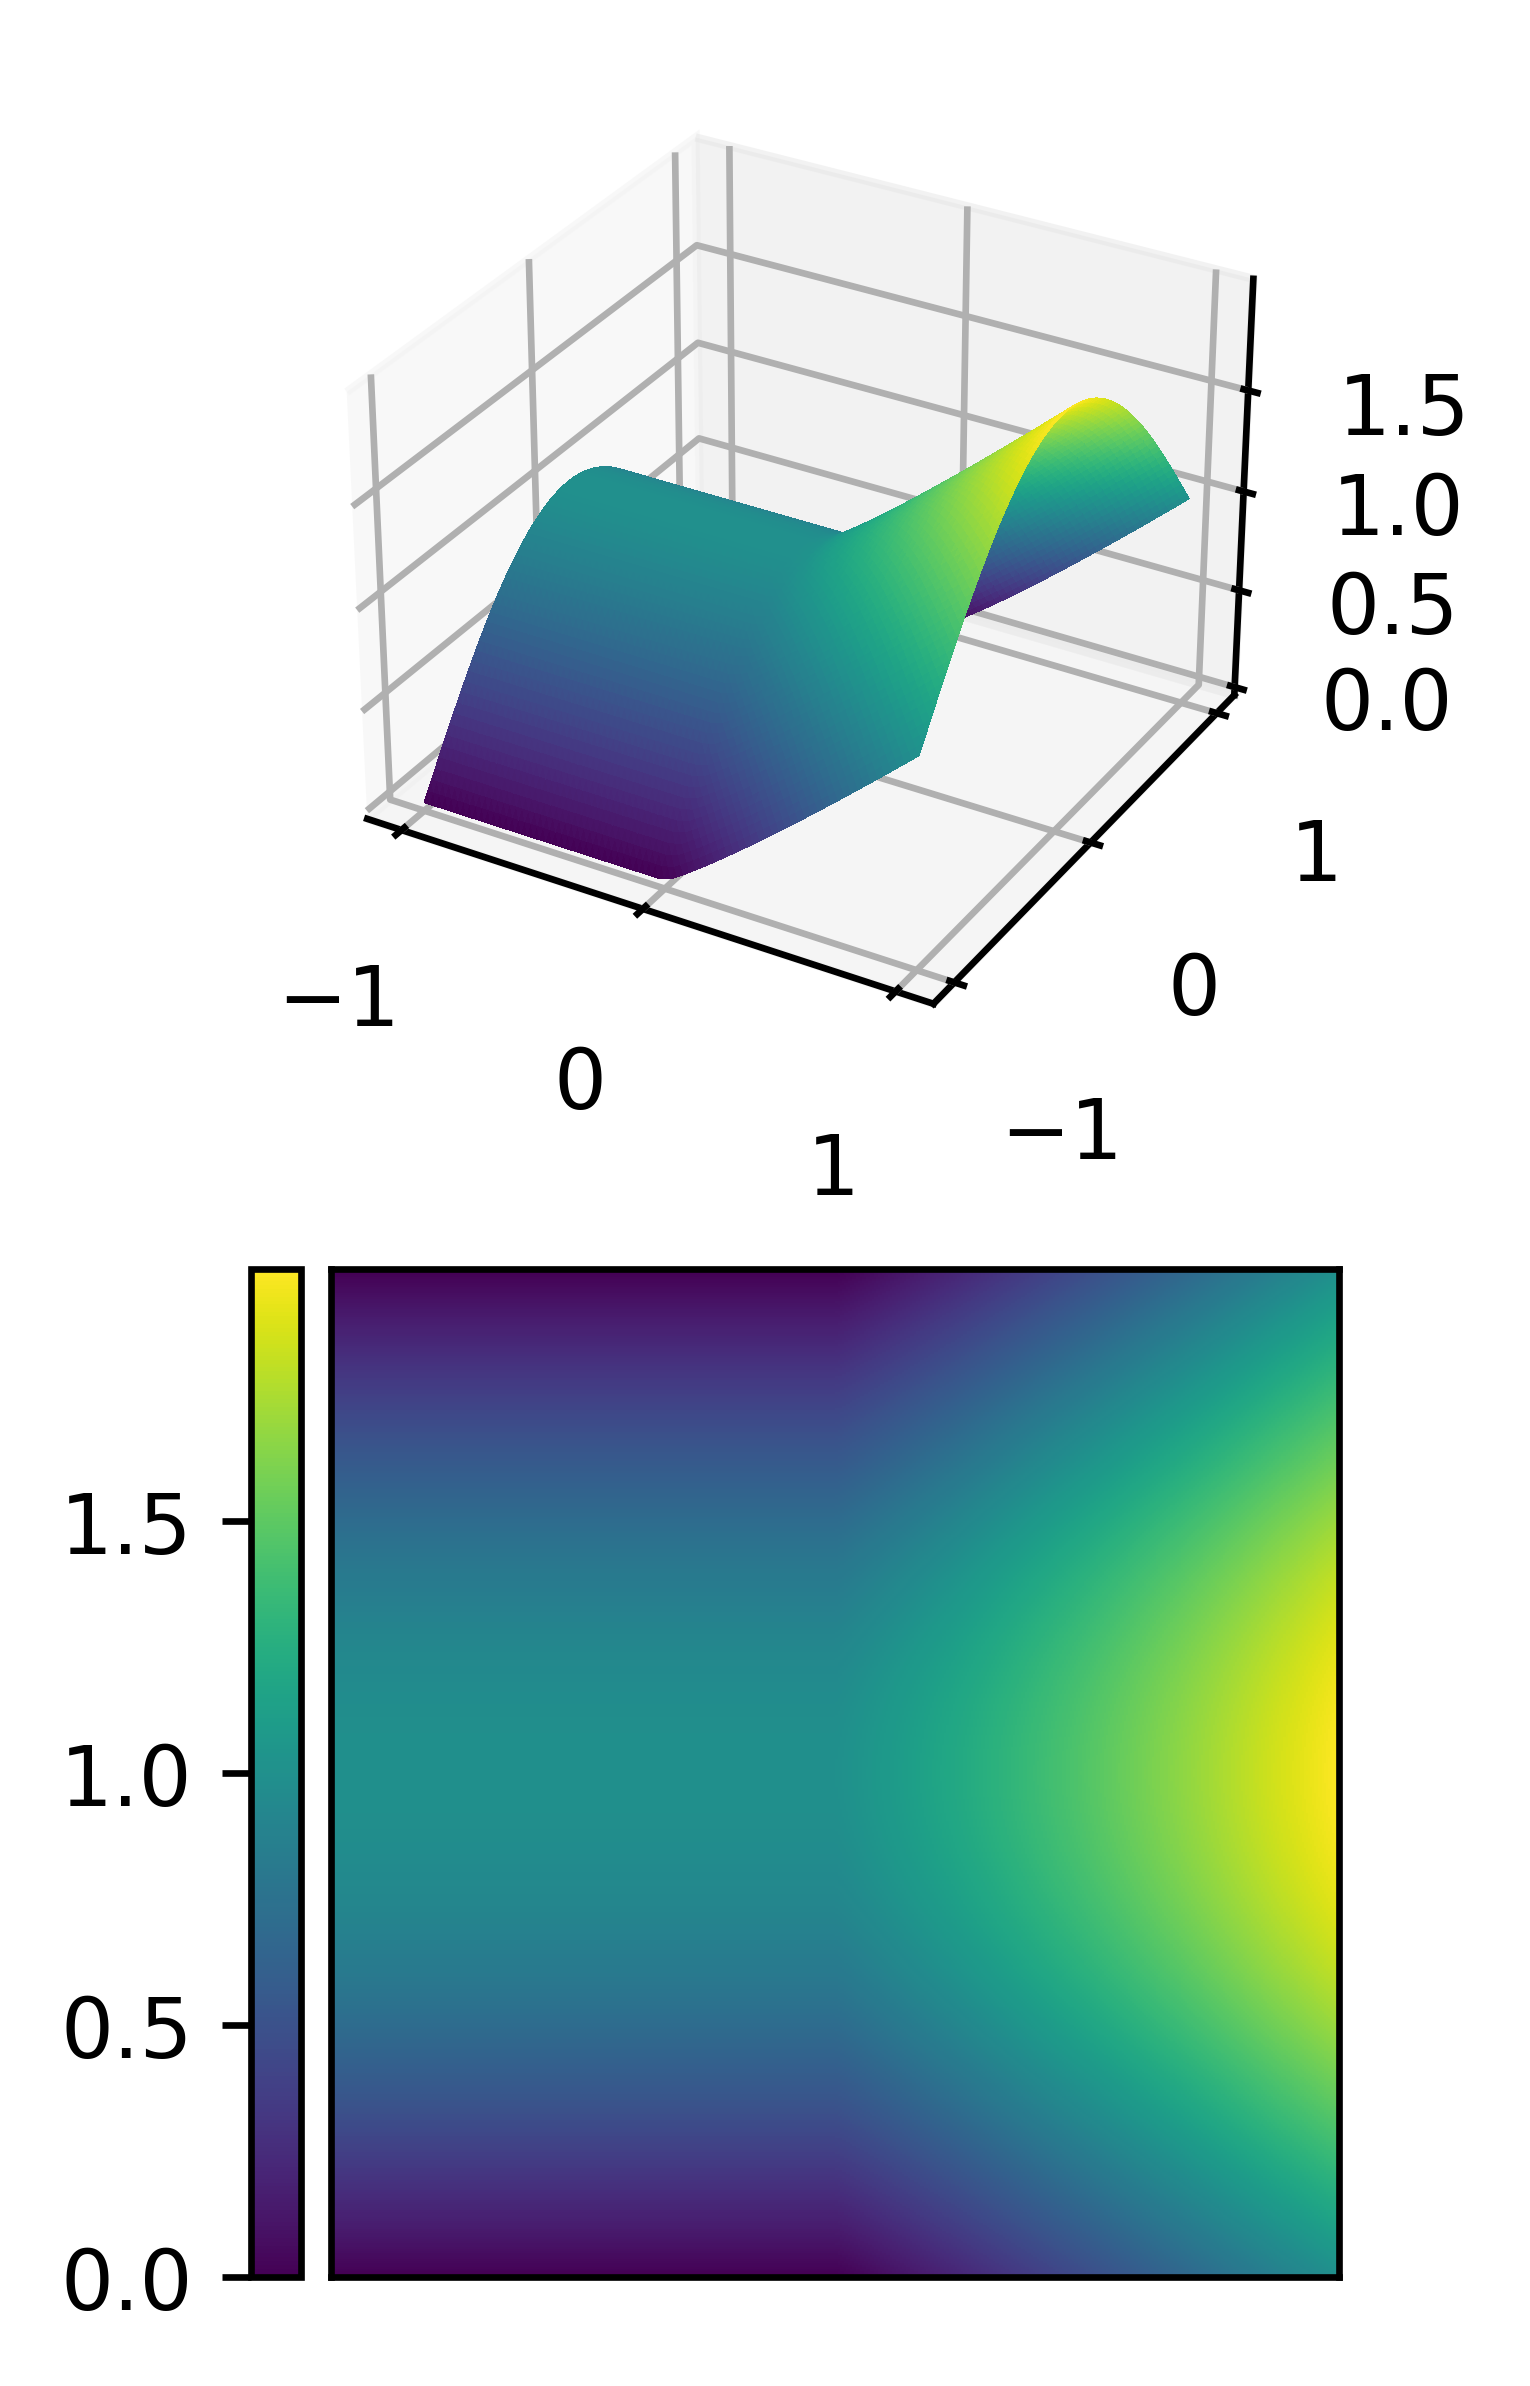
\includegraphics[width=.9\linewidth]{contour_nonsmooth_1}
    \caption{$a = 1.1$}
  \end{subfigure}%
  \begin{subfigure}{.5\linewidth}
    \centering
    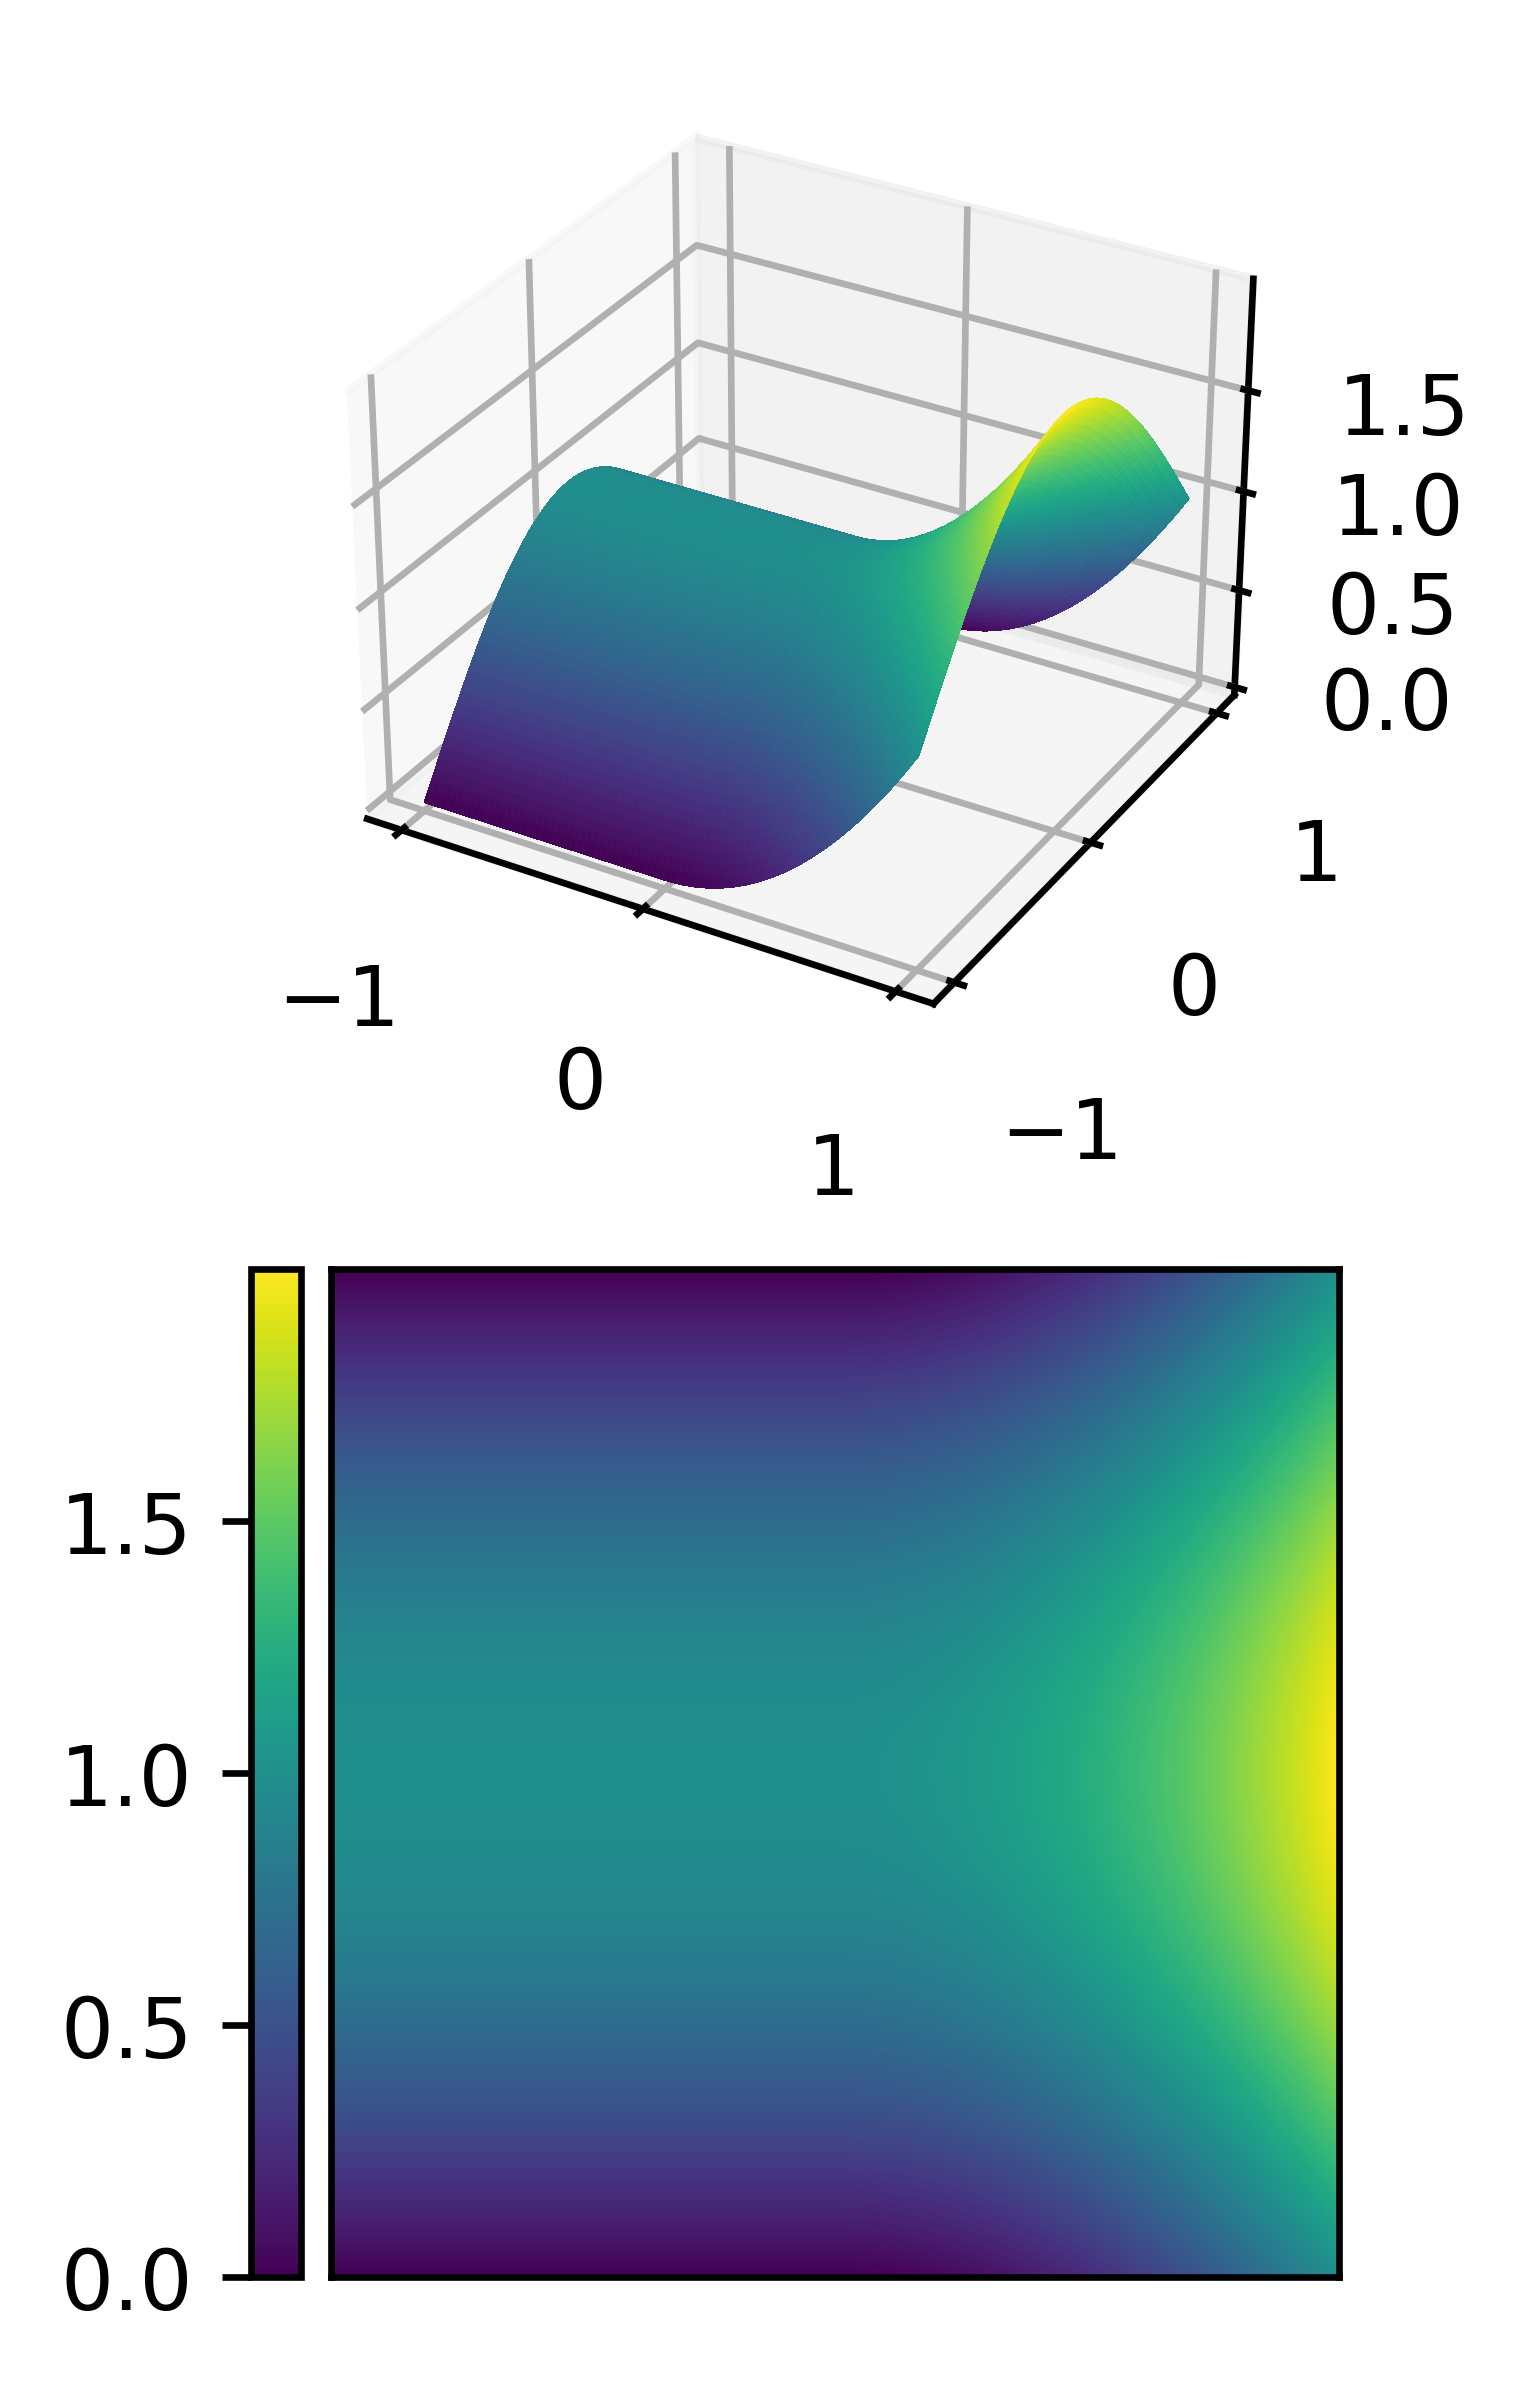
\includegraphics[width=.9\linewidth]{contour_nonsmooth_2}
    \caption{$a = 2$}
  \end{subfigure}
  \caption{Solution $u$ with varying parameter $a$}
  \label{fig:non_smooth_mixed_solution}
\end{figure}

In the $H^1$ semi-norm, linear convergence is expected for $1.5 < a$.
For $1 < a \le 1.5$ we have $u \notin H^2(\Omega)$ and linear convergence in the $L^2$ norm at best.
And for $1.5 < a$ quadratic convergence in the $L^2$ norm at best.
However, the theorem guaranteeing a convergence estimates in its precise form states:
\begin{multline}
    \exists n \in \mathbb{N}: \, \lVert u - u_h \rVert_{L^2} \in \mathcal{O}\left(h\right), \\ \forall h < \frac{1}{n}, u \in H^1(\Omega)
\end{multline}
\begin{multline}
    \exists n \in \mathbb{N}: \, \lVert u - u_h \rVert_{L^2} \in \mathcal{O}\left(h^2\right), \\ \forall h < \frac{1}{n}, u \in H^2(\Omega)
\end{multline}
This threshold is likely to increase with less regularity of the solution. So a more natural
expectation is for the convergence rate to increase with increasing $a$.


Exactly linear convergence is observed in \autoref{fig:err_nonsmooth_h1} for the $H^1$ semi-norm and $1.5 < a$.
For $a = 1.3$, it still appears to converge but at a rate of $\mathcal{O}\left(h^{0.6}\right)$.

In \autoref{fig:err_nonsmooth_l2} it can be observed how the convergence rate depends on the regularity of the solution.
For the highly irregular solution with $a = 1.3$, linear convergence is only given during the first steps.
A similar behaviour is observed for $1.5 < a < 2.2$ where quadratic convergence is expected, but only given
during the first steps.
Truly quadratic convergence can only be observed for $2.2 < a$.
The estimated convergence rates are not exactly observed for the borderline cases.
This could be a hint to the fact that our estimates should be improved, or the needed threshold from where on the
convergence sets in is not reached if the function is only just in the needed space.

\begin{figure}[H]
  \centering
  \begin{subfigure}{1\linewidth}
    \centering
    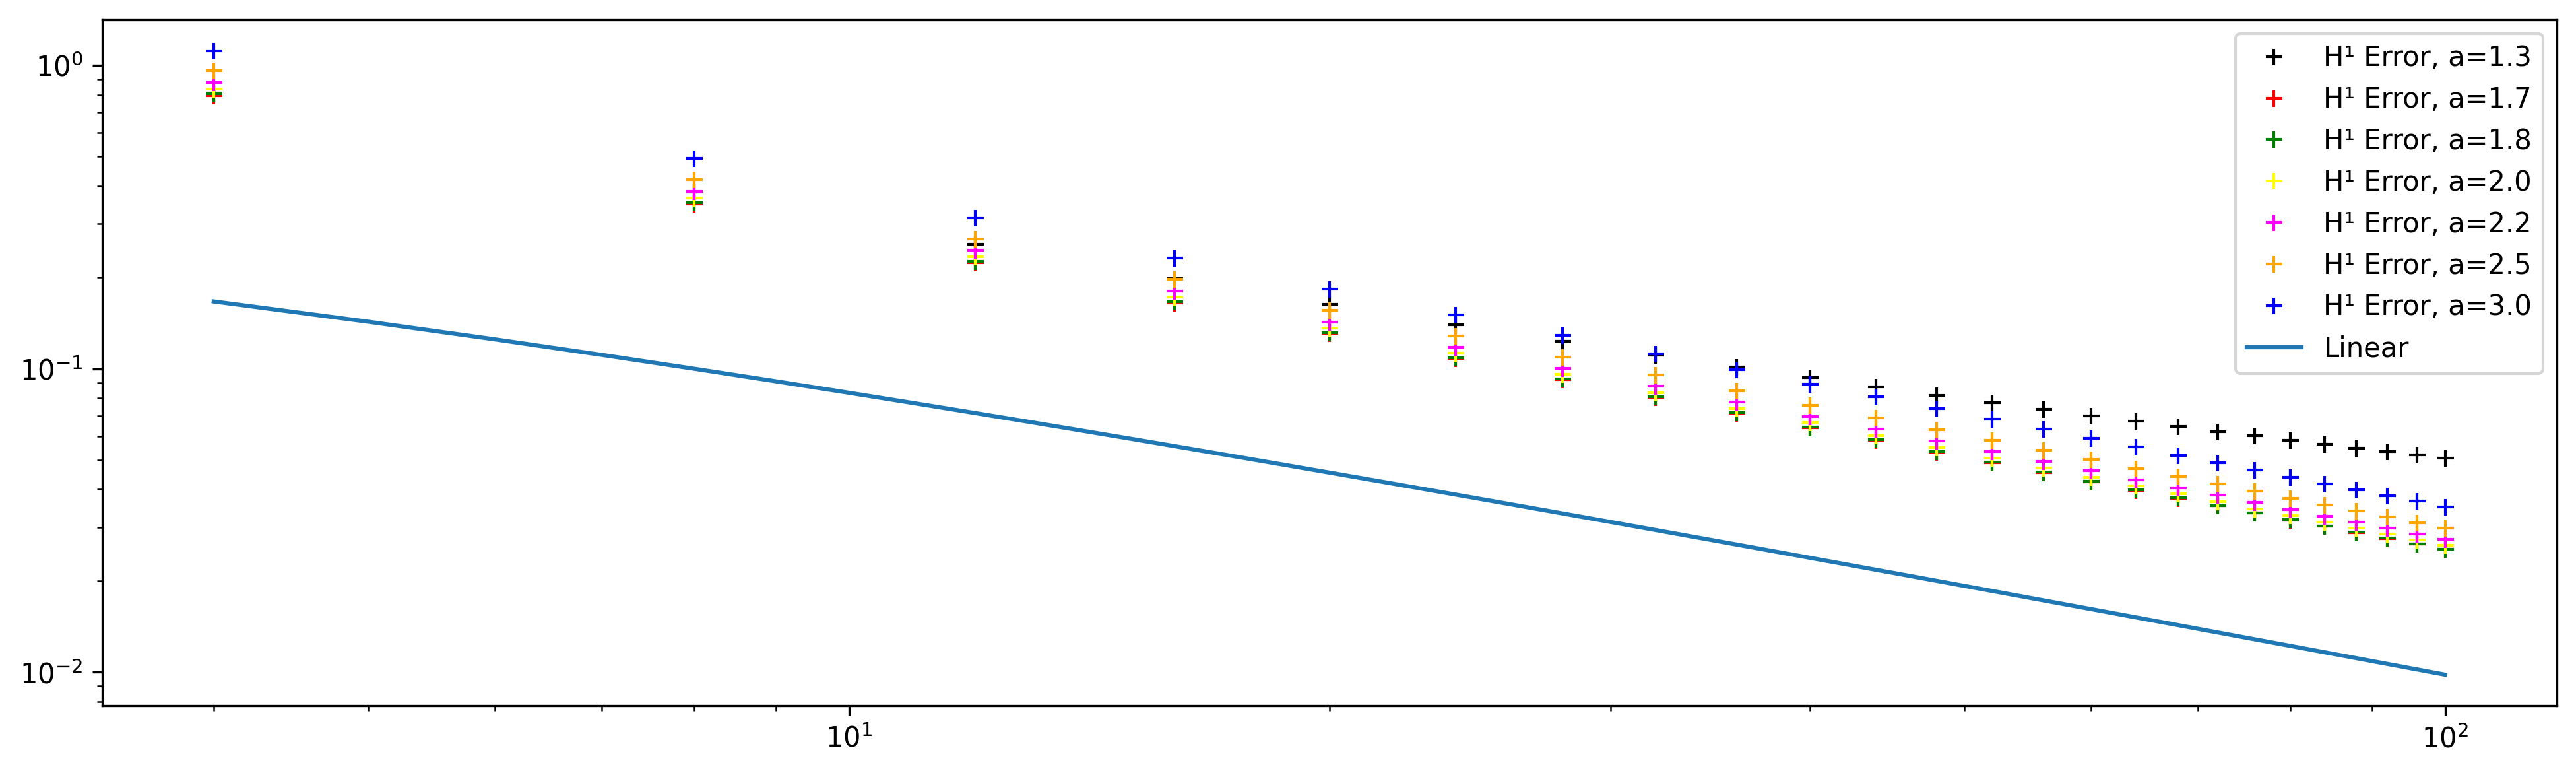
\includegraphics[width=.8\linewidth]{errors_nonsmooth_h1}
    \caption{Convergence in the $H^1$ Semi-Norm}
    \label{fig:err_nonsmooth_h1}
  \end{subfigure}

  \begin{subfigure}{1\linewidth}
    \centering
    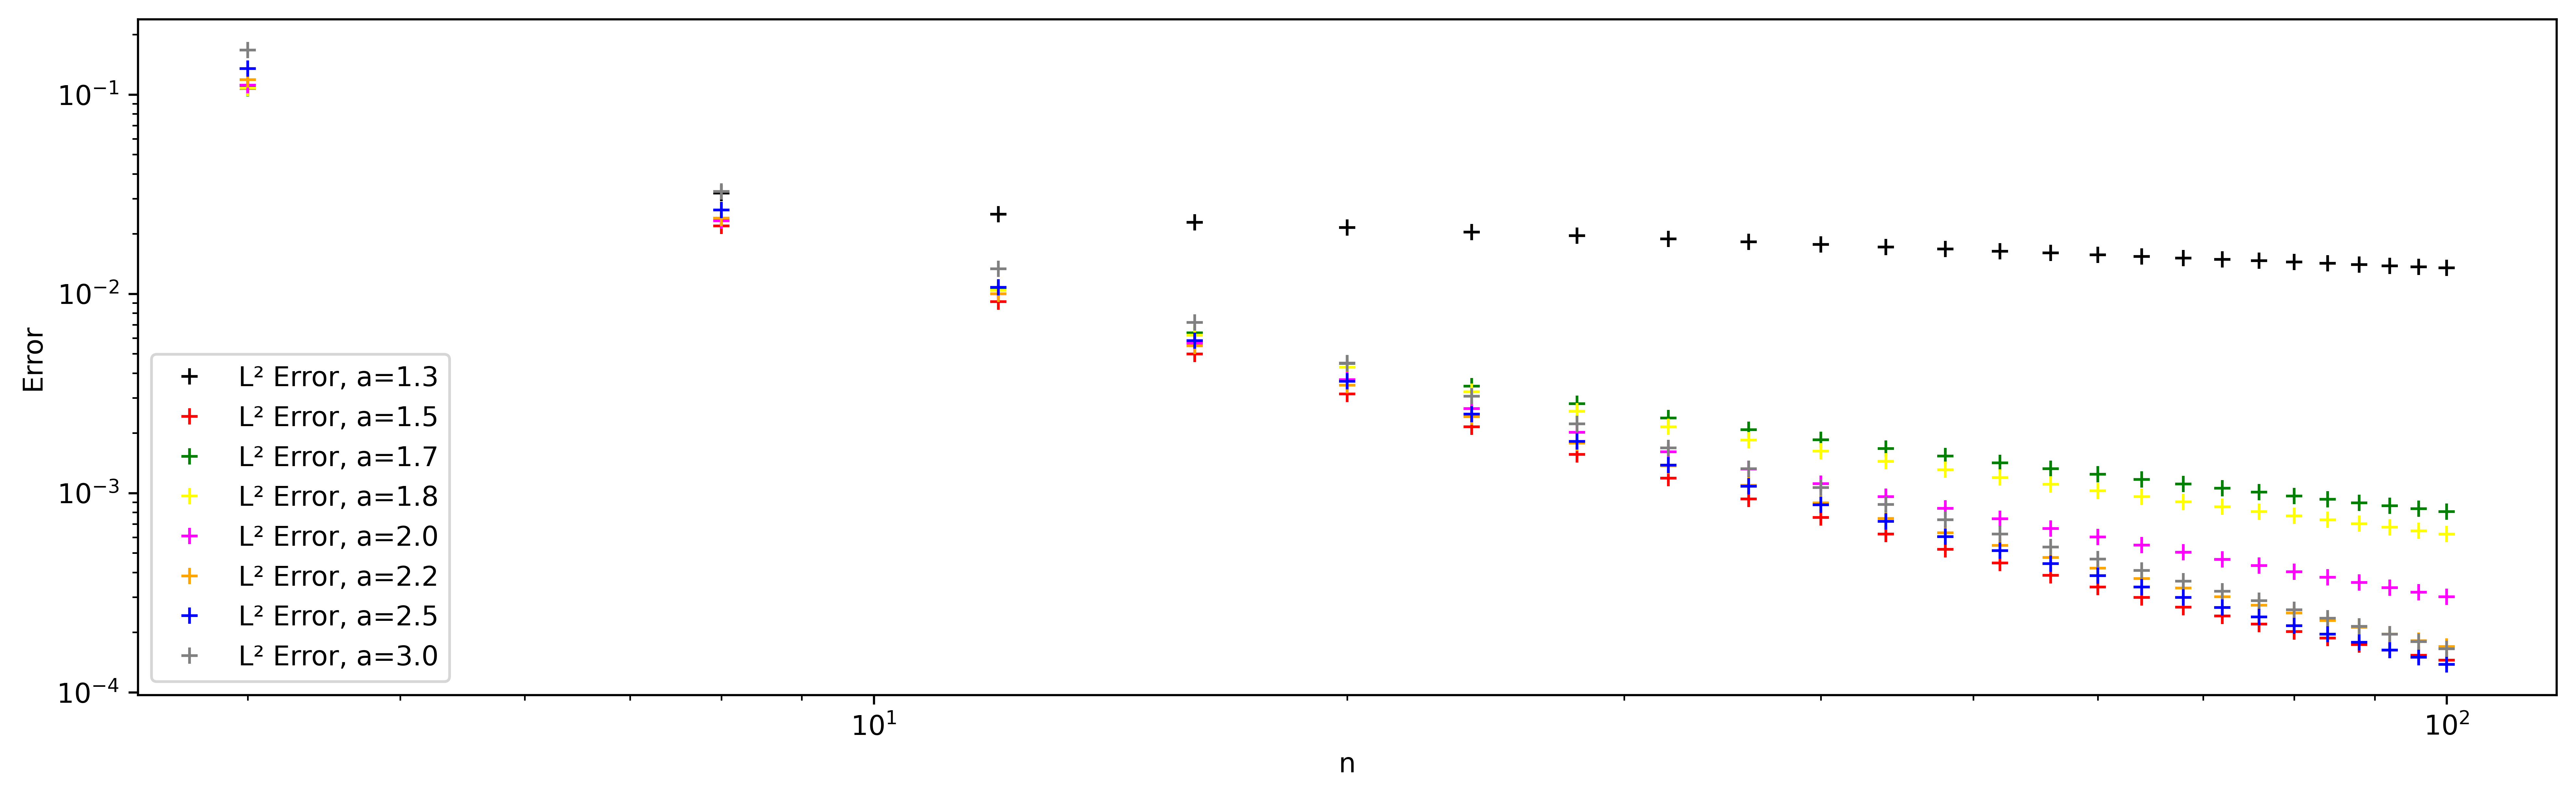
\includegraphics[width=.8\linewidth]{errors_nonsmooth_l2}
    \caption{Convergence in the $L^2$ Norm}
    \label{fig:err_nonsmooth_l2}
  \end{subfigure}
  \caption{Convergence With Varying Regularity of the Solution}
\end{figure}


\subsection*{Higher Order Elements}
To increase the accuracy of the solution on a coarser mesh, a polynomial basis
of higher order can be chosen.
This may be achieved by considering higher order local basis functions defined on the reference element.
So far, linear basis functions had been considered. These local basis functions are visualized in \autoref{fig:p1_2d_mesh_basis}.
\begin{figure}[H]
  \centering
  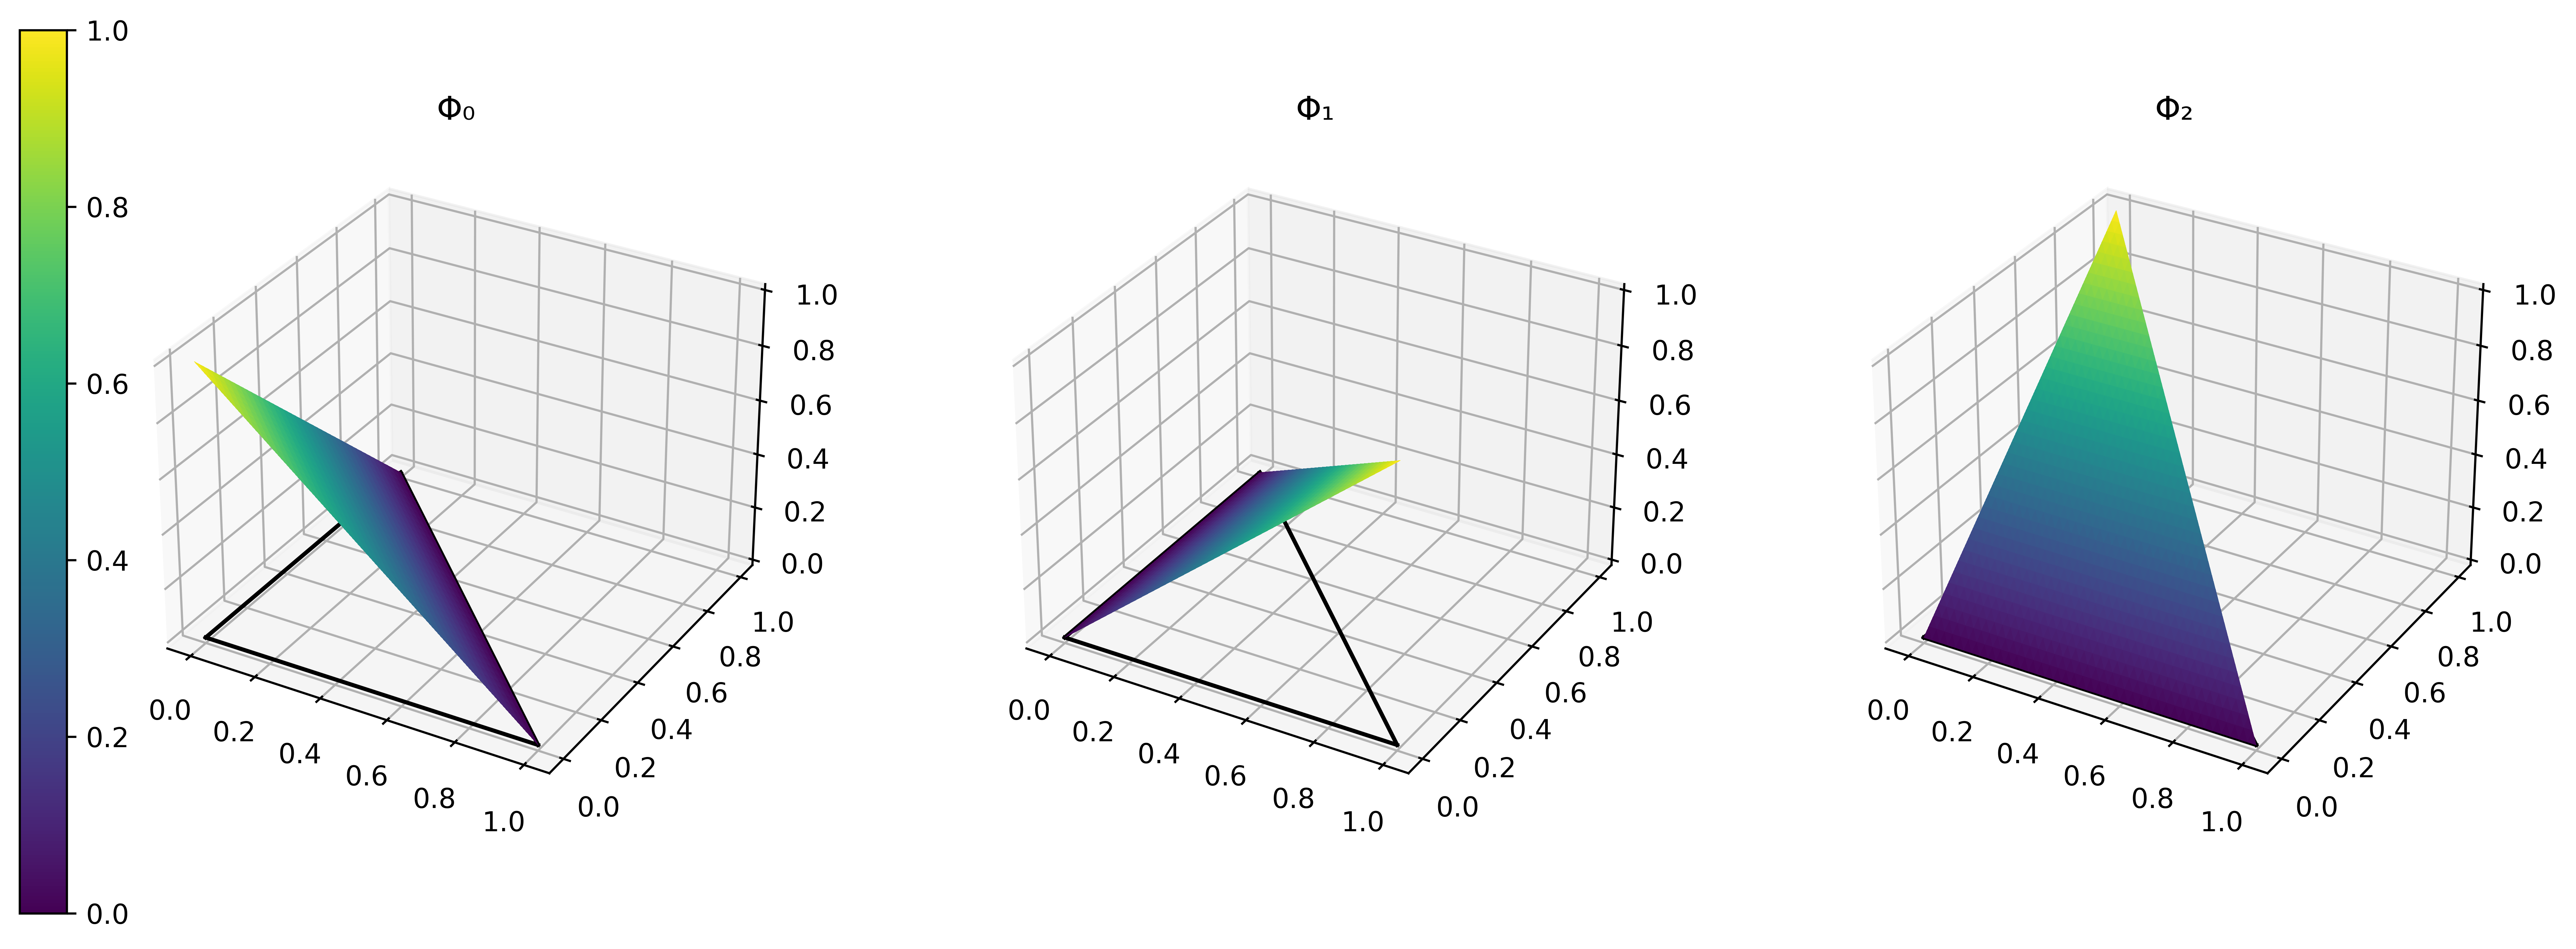
\includegraphics[width=.9\linewidth]{p1_2d_mesh_basis}
  \caption{Polynomial Basis of Degree 1 on 2-Simplex}
  \label{fig:p1_2d_mesh_basis}
\end{figure}

To obtain a basis for the entire space on the mesh, those local basis functions are mapped to each simplex.
Global continuity is ensured by joining enough nodes on the boundaries of adjacent simplexes.
3 basis functions of the function space defined on the entire mesh are visualized in \autoref{fig:p1_2d_stitch_basis}.
\begin{figure}[H]
  \centering
  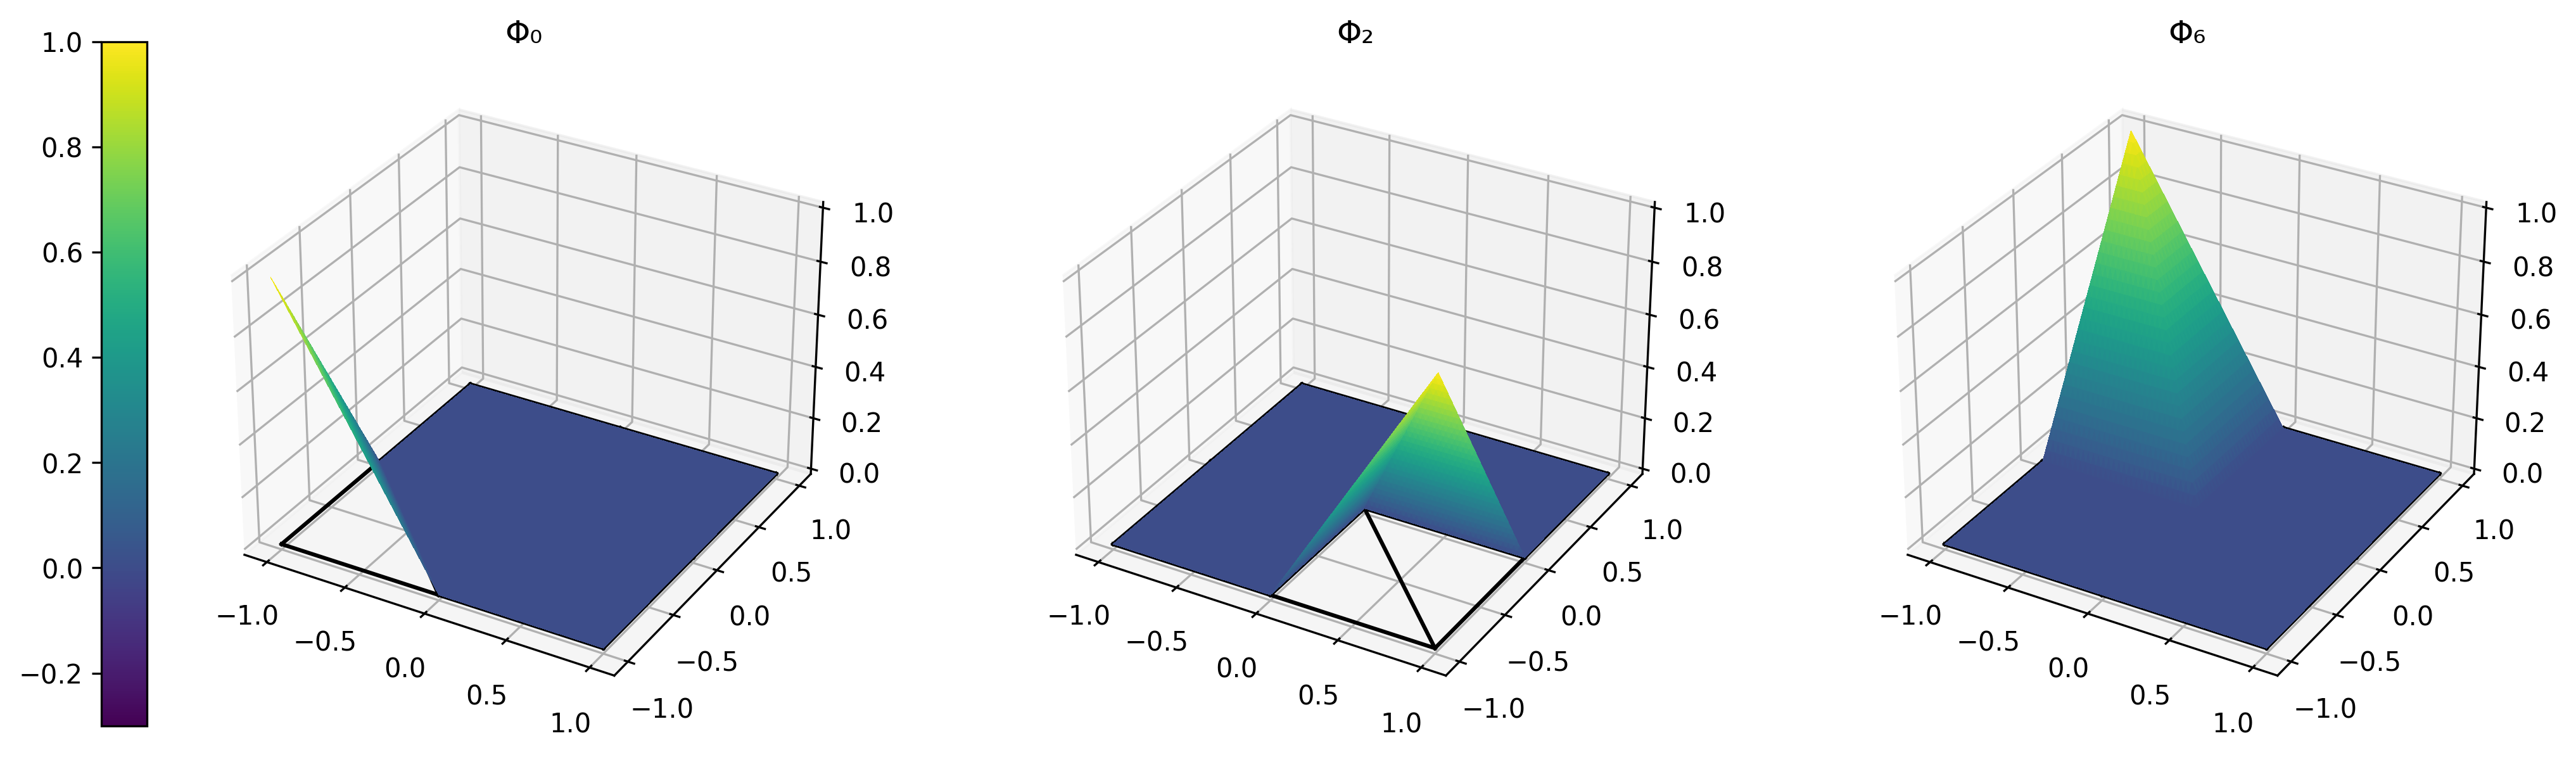
\includegraphics[width=.9\linewidth]{p1_2d_stitch_basis}
  \caption{3 Piecewise Linear Basis Functions of the Function Space defined on the entire Grid}
  \label{fig:p1_2d_stitch_basis}
\end{figure}


Generalizing this approach to higher order Polynomials requires the definition of higher order polynomial
basis functions on the reference element. For this
$$N_p = \frac{(p+d)!}{p! \cdot d!}$$
nodes have to be chosen on each element. Where $p$ is the degree of the polynomial basis and $d$ is the spatial dimension.

To ensure regularity along adjacent simplexes on the mesh,
$$\tilde{N}_{p} = \frac{(p+(d-1))!}{p!\cdot(d-1)!}$$
nodes have to lie on each boundary segment of the reference simplex.

Exemplary local basis functions for $p=2$ and $p=3$ are visualized in \autoref{fig:higher_order_basis}.
\begin{figure}[H]
  \centering
  \begin{subfigure}{.49\linewidth}
    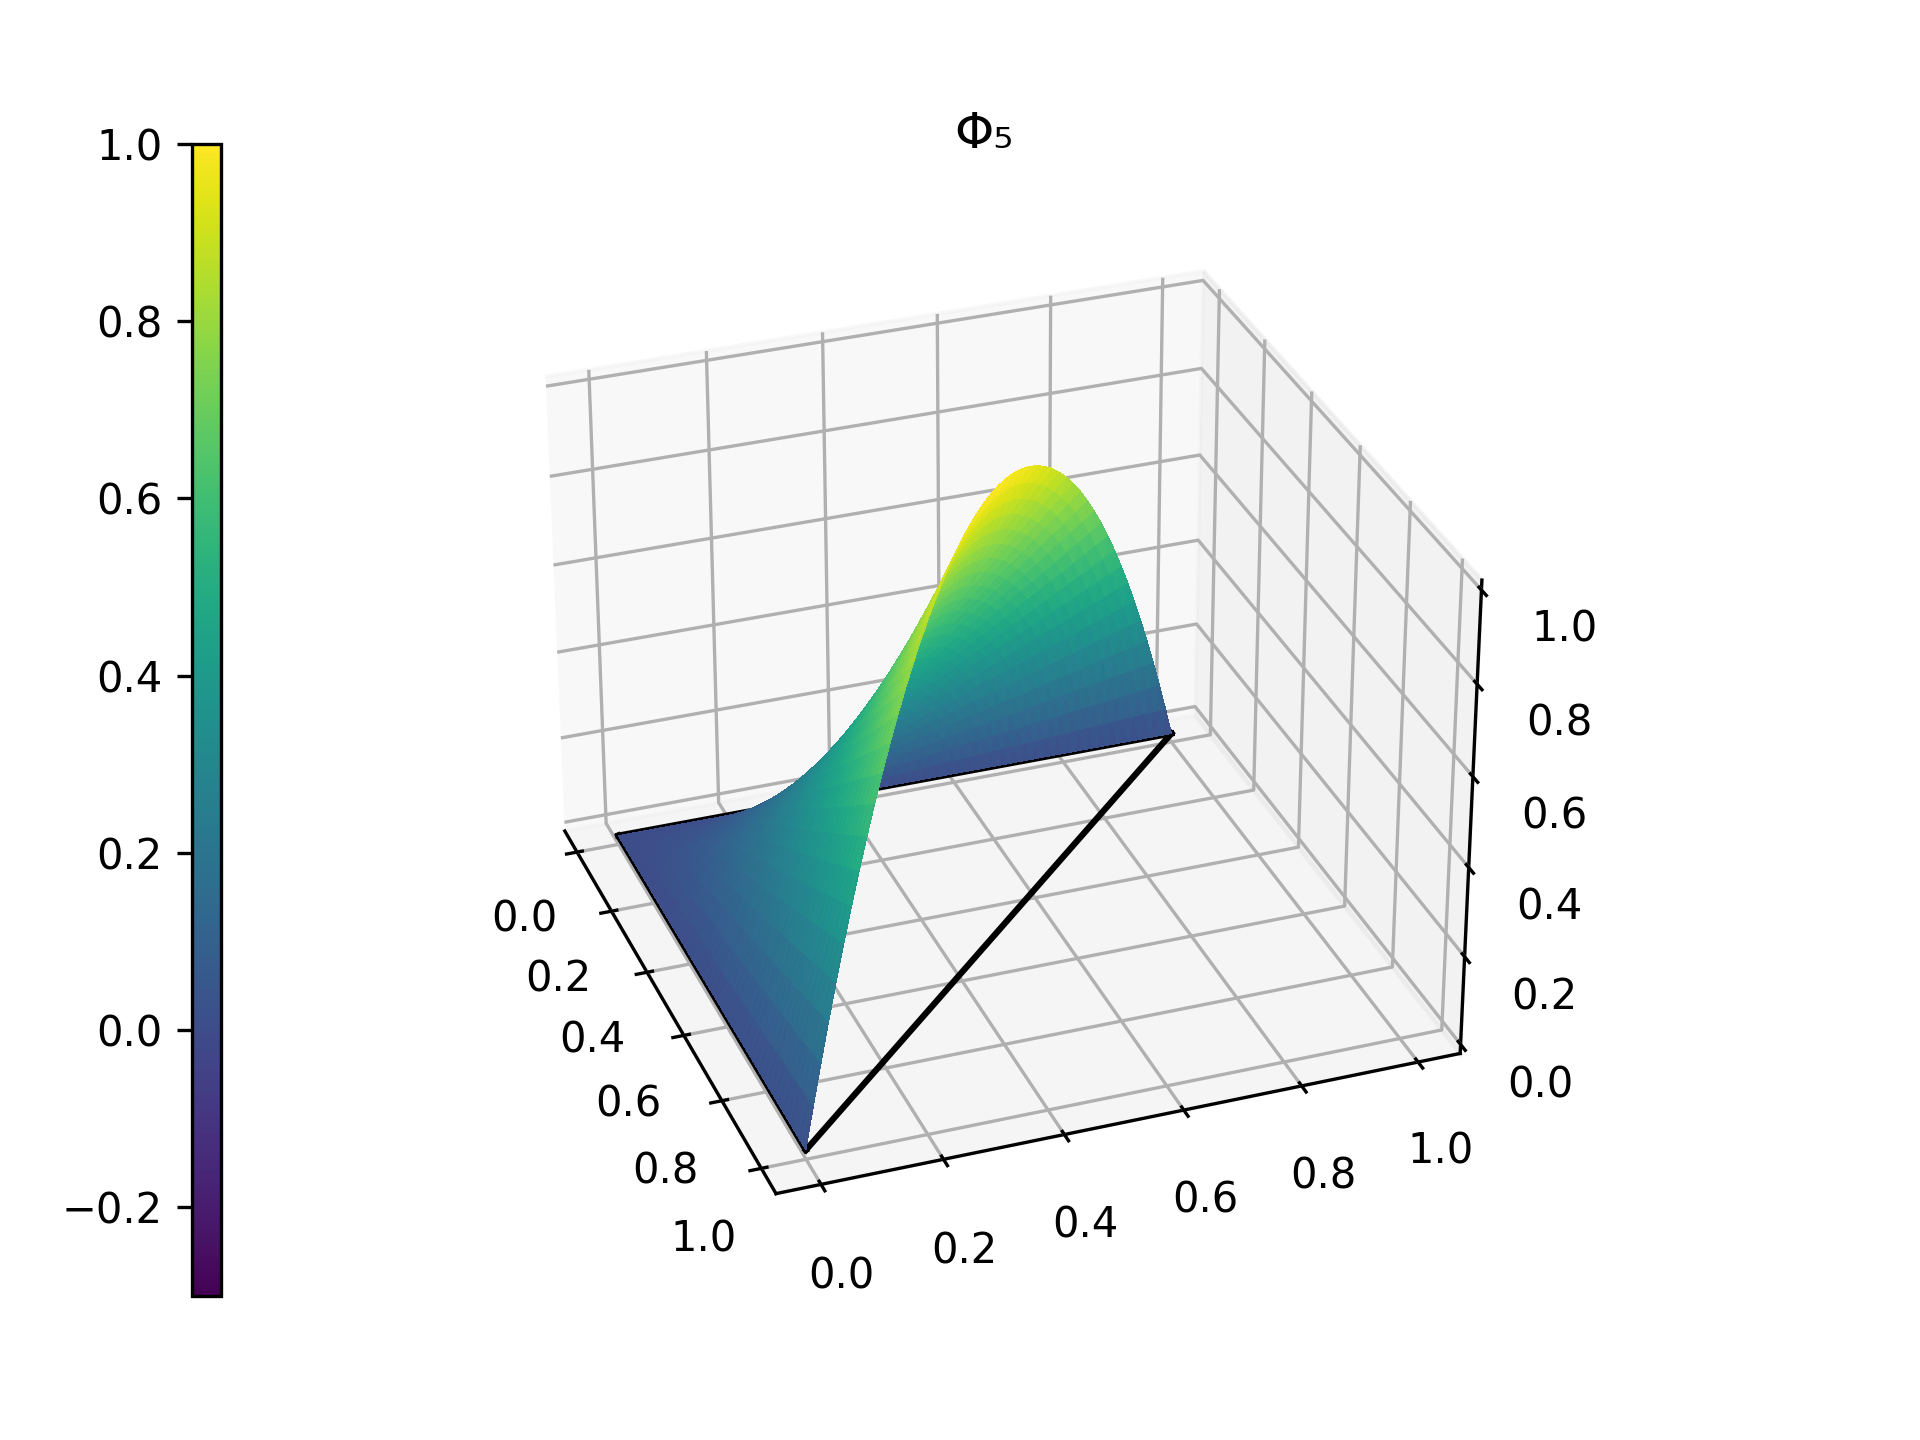
\includegraphics[width=1\linewidth]{p2_basis}
    \caption{$p=2$ Local Basis Function}
  \end{subfigure}\hfill%
  \begin{subfigure}{.49\linewidth}
    \raggedright
    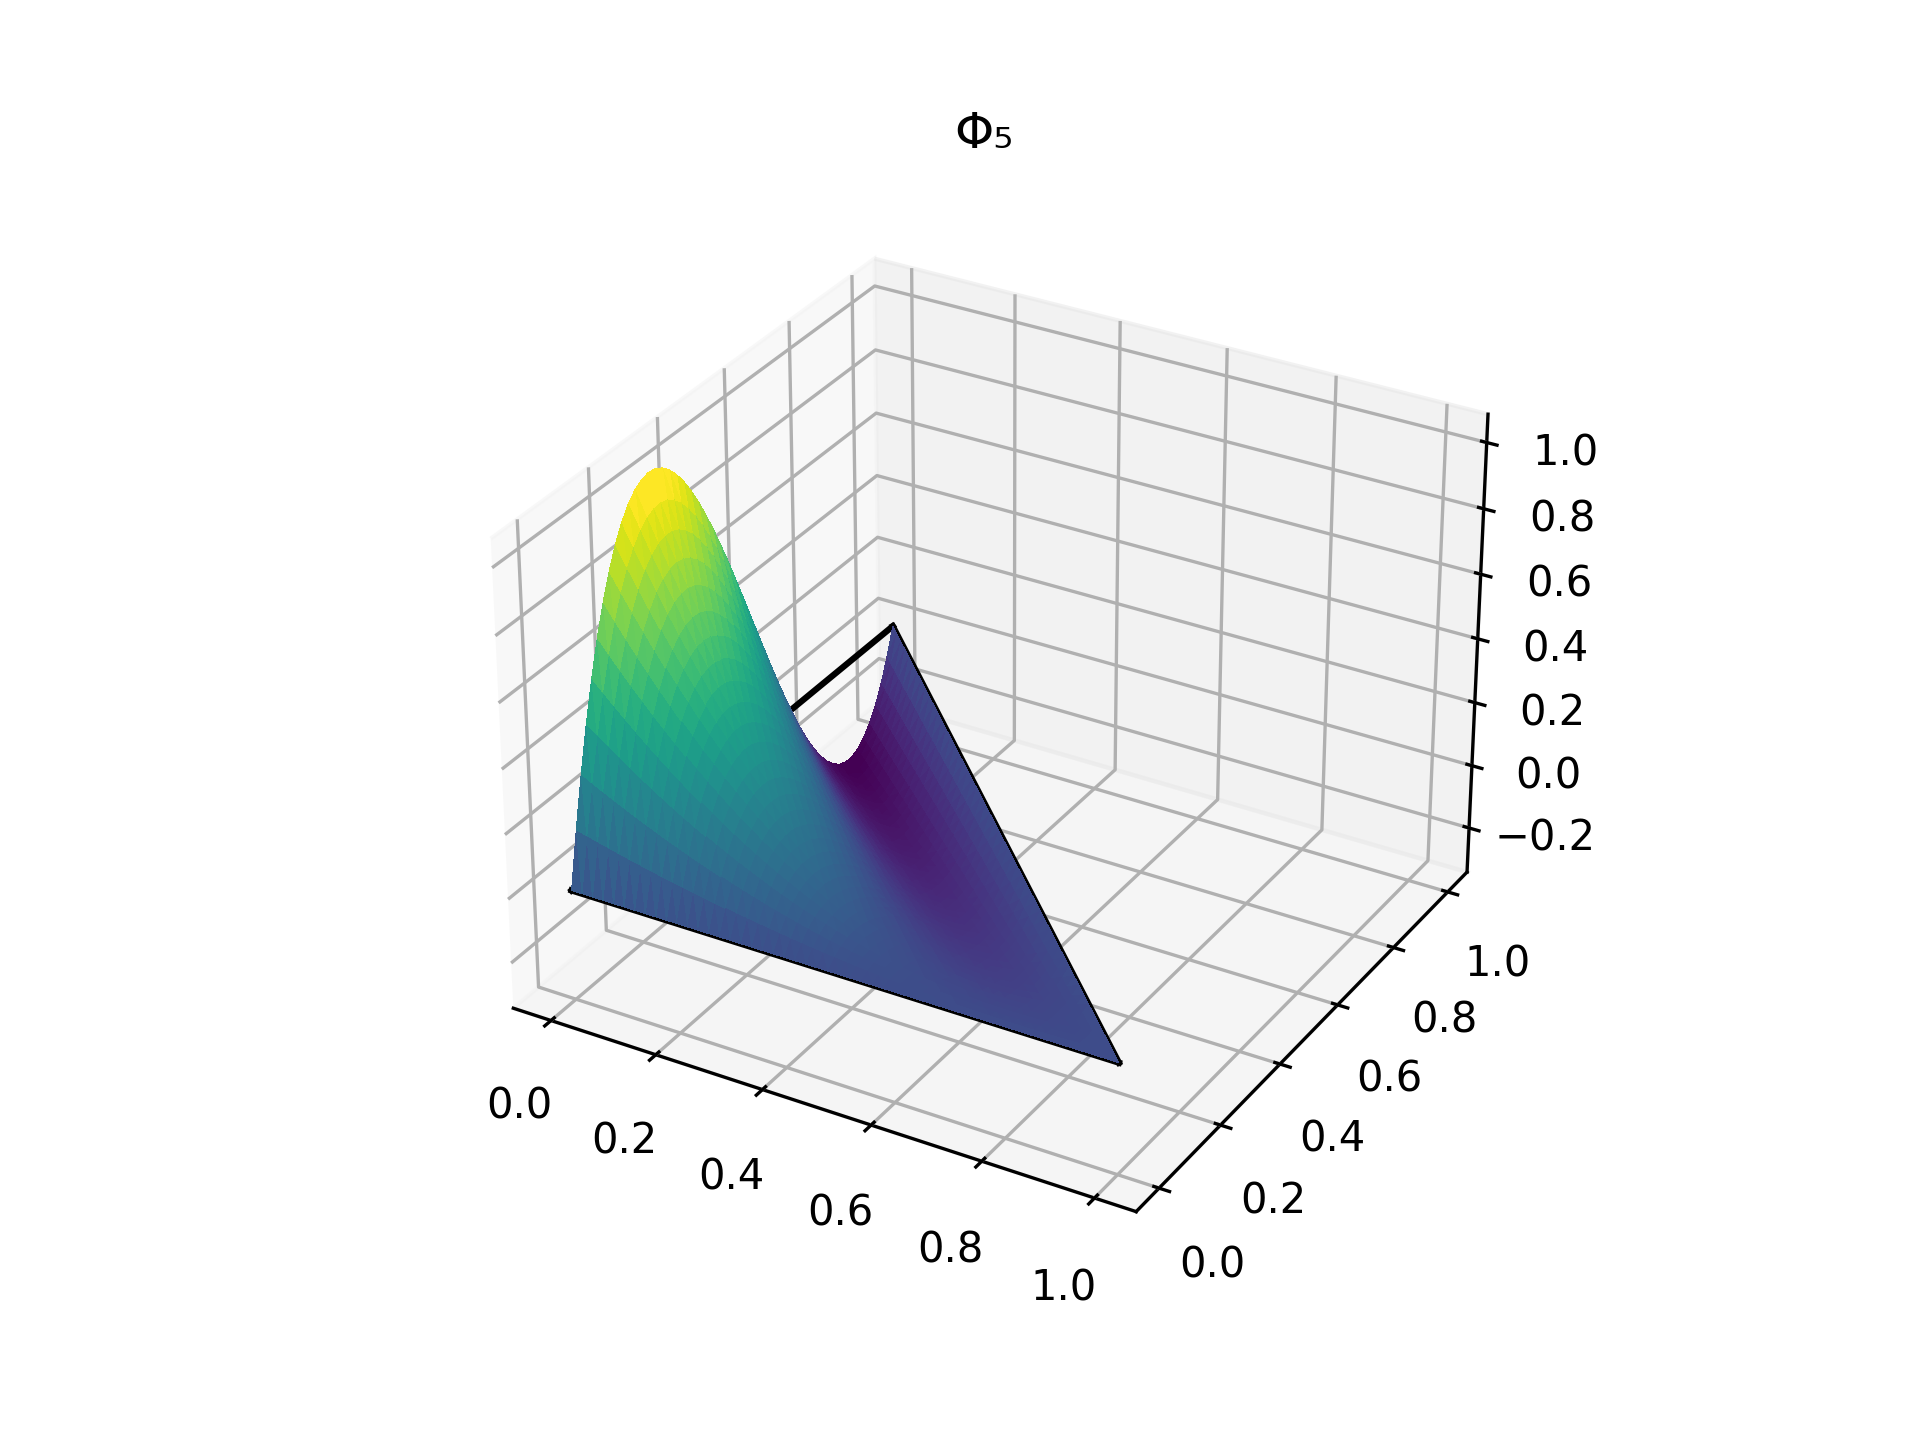
\includegraphics[width=1\linewidth]{p3_basis}
    \caption{$p=3$ Local Basis Function}
  \end{subfigure}
  \caption{Higher Order Local Basis Functions}
  \label{fig:higher_order_basis}
\end{figure}

To compare how higher order elements perform compared to their linear counterparts,
the same numerical experiments as for the piecewise linears will be repeated with higher order elements.

The following estimate for the convergence rates of $p$\textsuperscript{th} order
elements has been established during the lecture:
\begin{equation}
  \label{eq:conv_high_order}
  \lVert u - u_h \rVert_{L^2} \lesssim h^{k'} \lVert u \rVert_{H^{k'+1}}
\end{equation}
Where $k' = \operatorname{min}\left(p,m\right)$ and $m$ is the largest integer s.t. $u \in H^{m+1}$.

By using Problem (\ref{eq:smooth_poisson_prob}) and (\ref{eq:poisson_less_smooth_prob})
again, the parameter $a$ can be adjusted easily to verify the above convergence
rate for higher order elements.

\subsubsection*{Smooth Solutions}
Using the problem (\ref{eq:smooth_poisson_prob}) with $a = 5$ we have $u \in H^k(\Omega) \forall k \in \mathbb{N}$.
Thus, a convergence rate of $ \sim h^{p+1}$ for a polynomial basis of arbitrary degree $p$ in the $L^2$ norm is expected.
This is verified on a regular grid in \autoref{fig:err_smooth_highorder_l2}.
\begin{figure}[H]
  \centering
  \begin{subfigure}{1\linewidth}
    \centering
    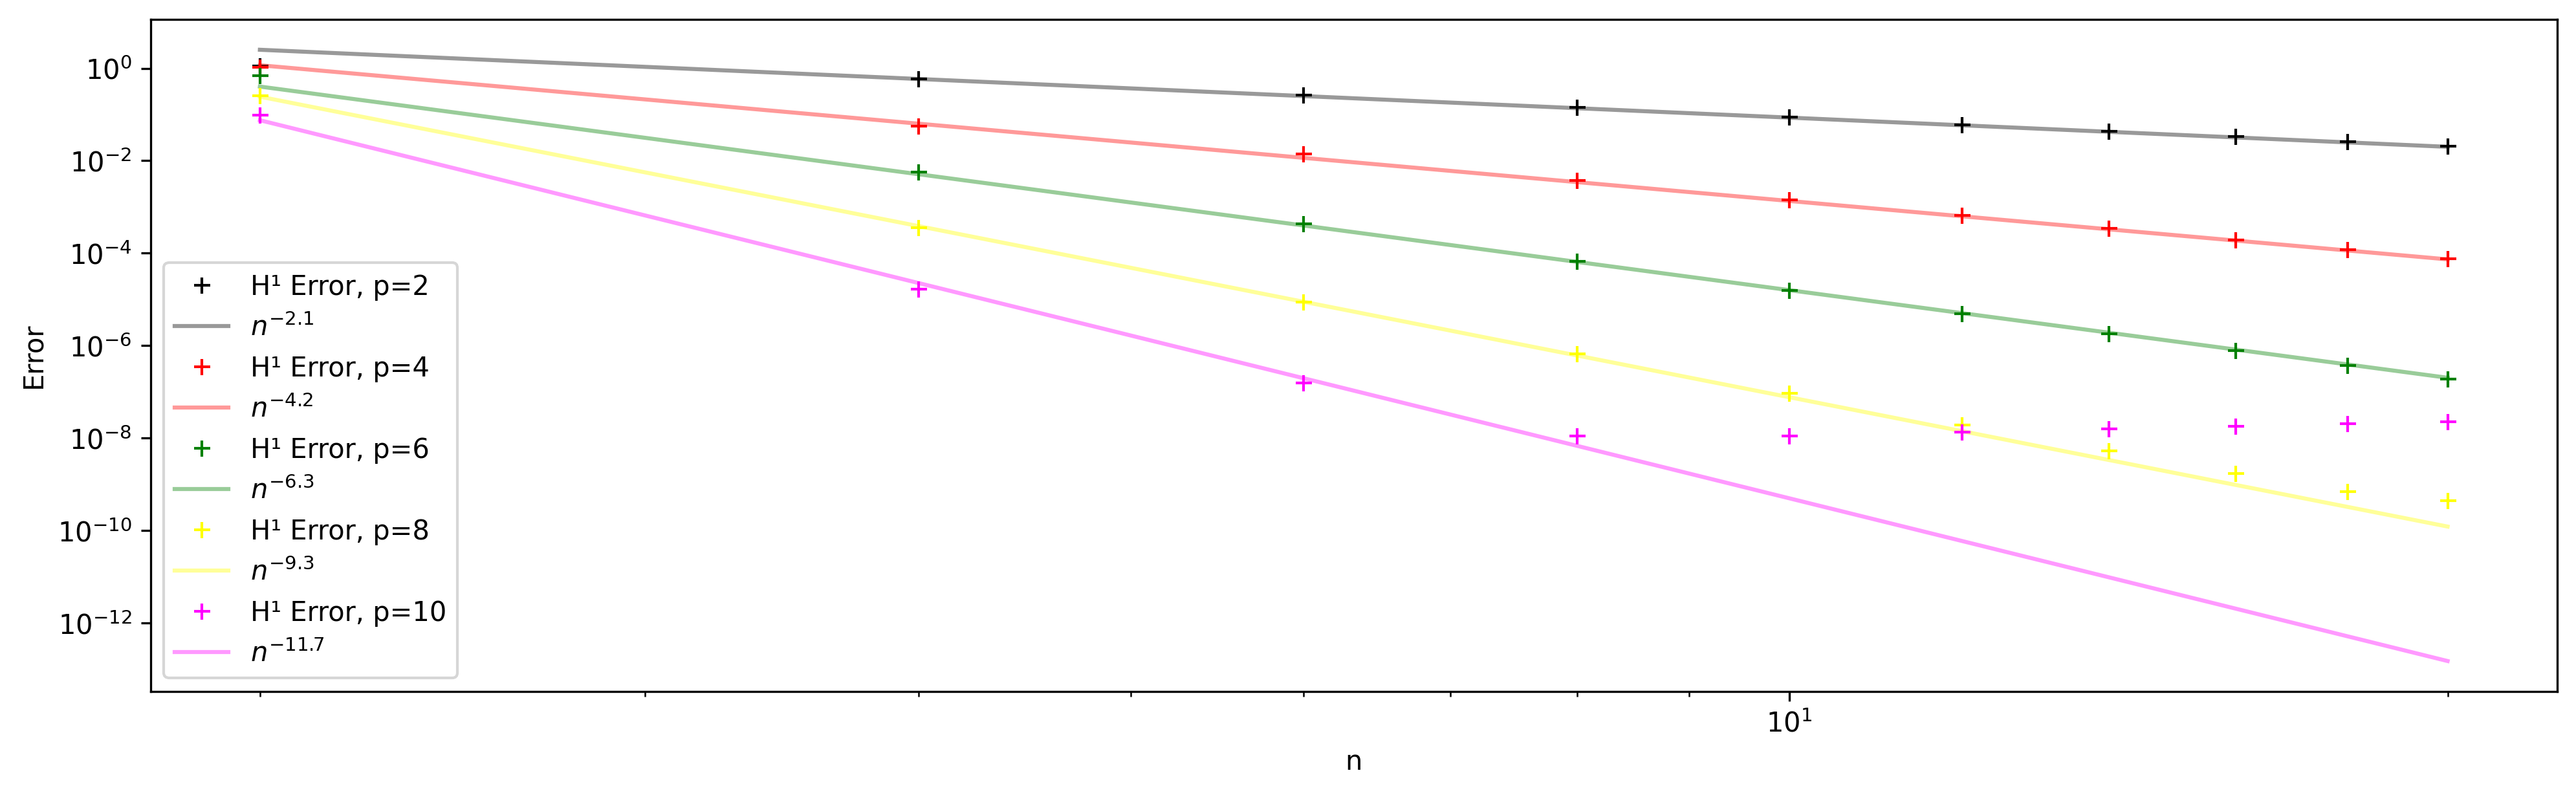
\includegraphics[width=.8\linewidth]{errors_smooth_highorder_h1}
    \caption{Convergence in the $H^1$ Semi-Norm}
    \label{fig:err_smooth_highorder_h1}
  \end{subfigure}

  \begin{subfigure}{1\linewidth}
    \centering
    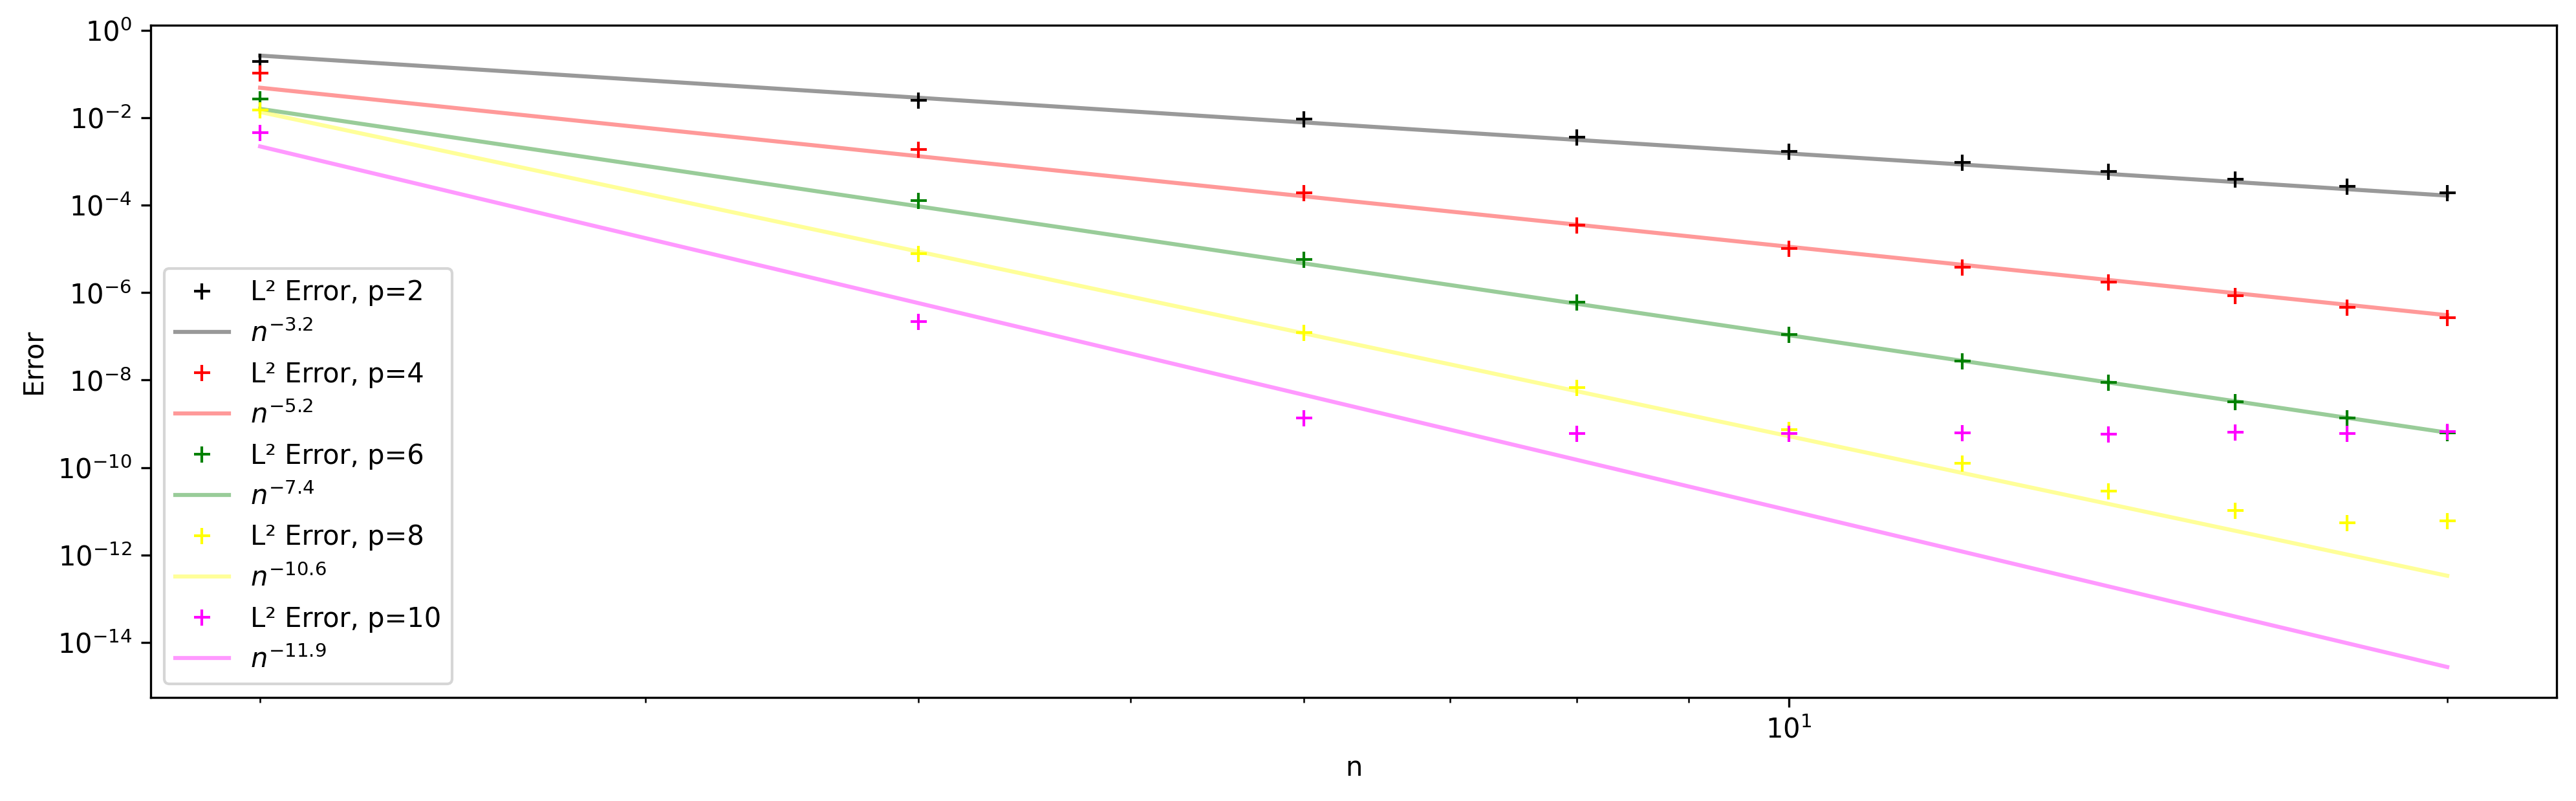
\includegraphics[width=.8\linewidth]{errors_smooth_highorder_l2}
    \caption{Convergence in the $L^2$ Norm}
    \label{fig:err_smooth_highorder_l2}
  \end{subfigure}
  \caption{Convergence With Smooth Solutions and Higher Order Elements}
\end{figure}

Although, no specific error bound for the $H^1$ semi-norm was given, the experiments in \autoref{fig:err_smooth_highorder_h1} suggest,
that under the same assumptions as in \autoref{eq:conv_high_order}, we see convergence in $H^1$ semi-norm
with one order less.

It can be observed, that basis functions of degree $8$ and $10$ do converge very fast.
However, they stop increasing in accuracy after just a few refinement steps which is probably due to other numerical errors
associated with bad conditioning of the Vandermonde matrix and its inverse used to evaluate the basis functions.

\subsubsection*{Varying Regularity}
By, again, considering Problem (\ref{eq:poisson_less_smooth_prob}) and altering $a$, the different
convergence rates for varying regularity can be studied for local bases of different degrees.
The convergence estimate (\ref{eq:conv_high_order}) tells that for less regular solutions,
the convergence rate is not expected to increase when using higher order polynomials.
This is observed in \autoref{fig:err_ridge_l2}.


As in the smooth case, convergence in the $H^1$ semi-norm is also given at one order less than in the $L^2$ norm.
Even though no such convergence rate had been theoretically established.
\begin{figure}[H]
  \centering
  \begin{subfigure}{1\linewidth}
    \centering
    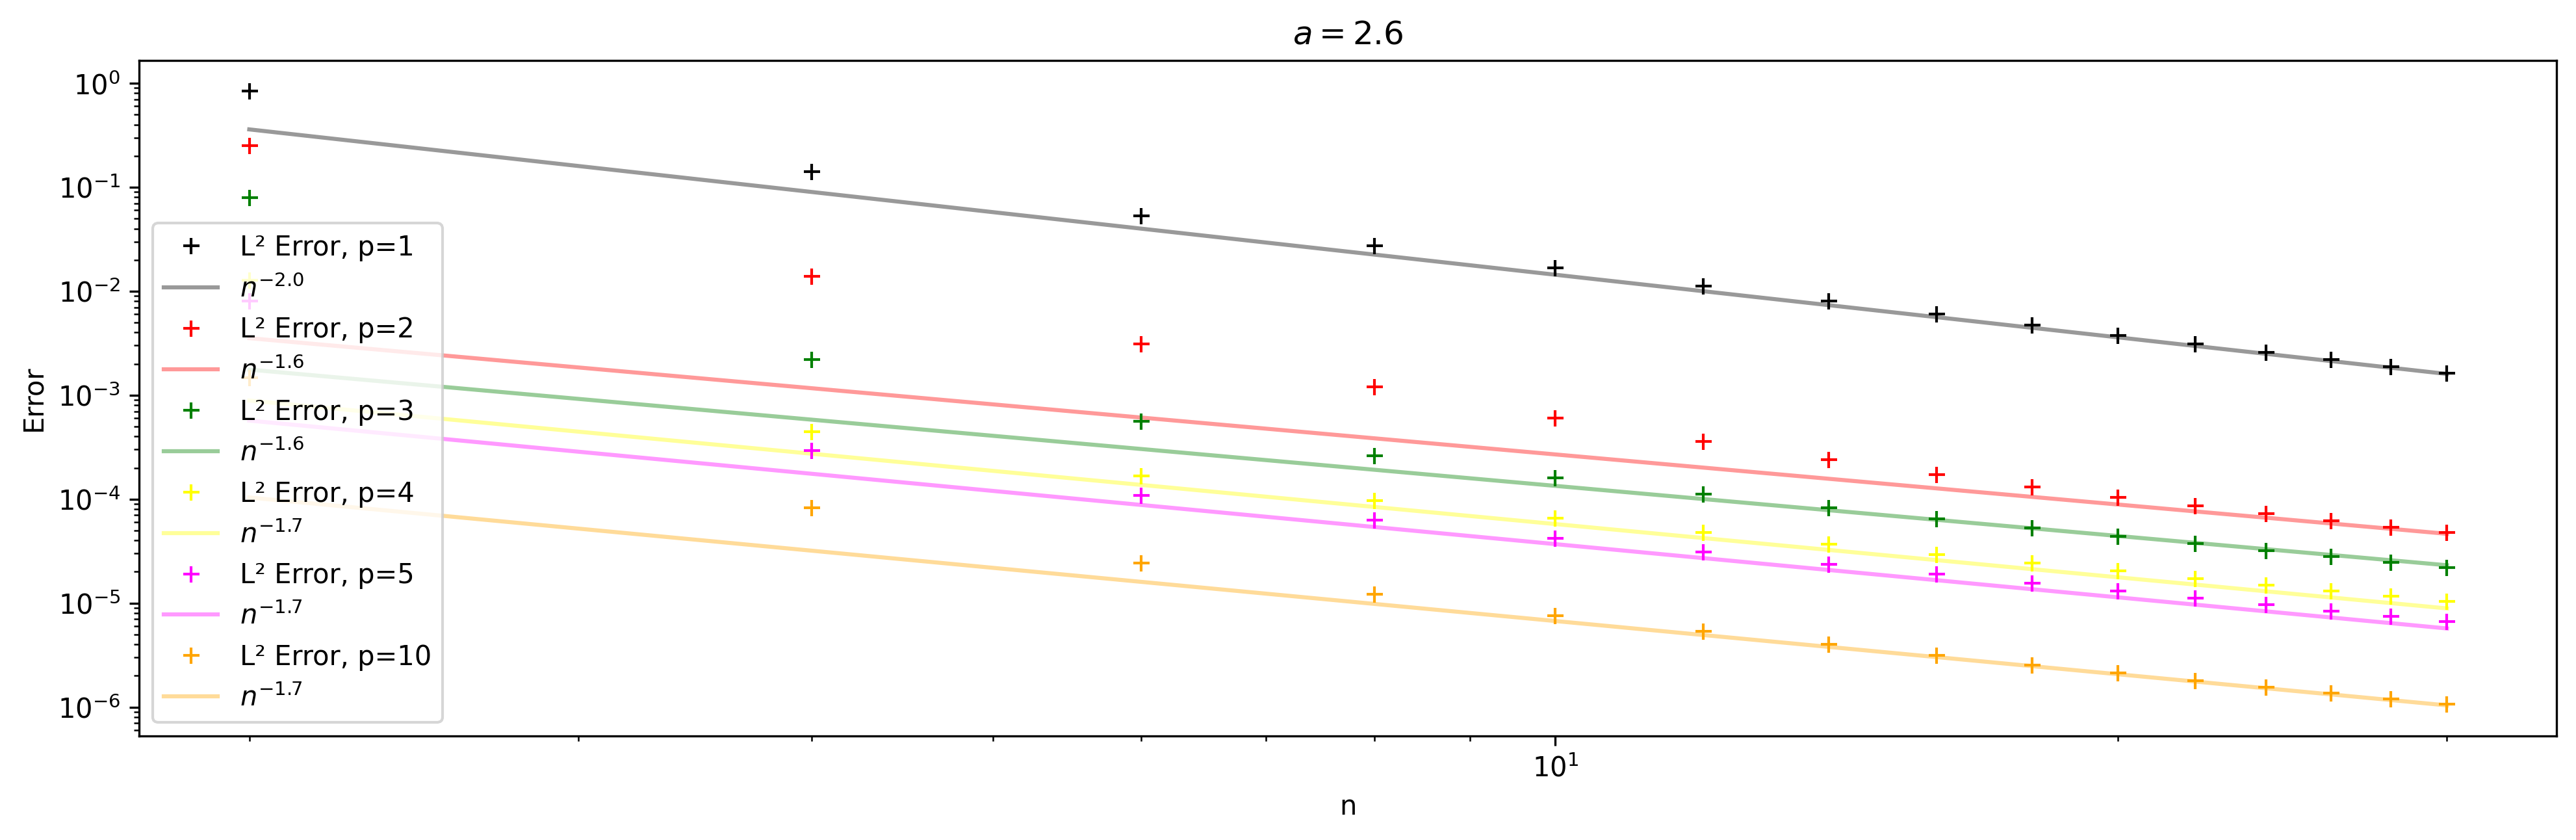
\includegraphics[width=.8\linewidth]{errors_ridge_26_l2}
  \end{subfigure}

  \begin{subfigure}{1\linewidth}
    \centering
    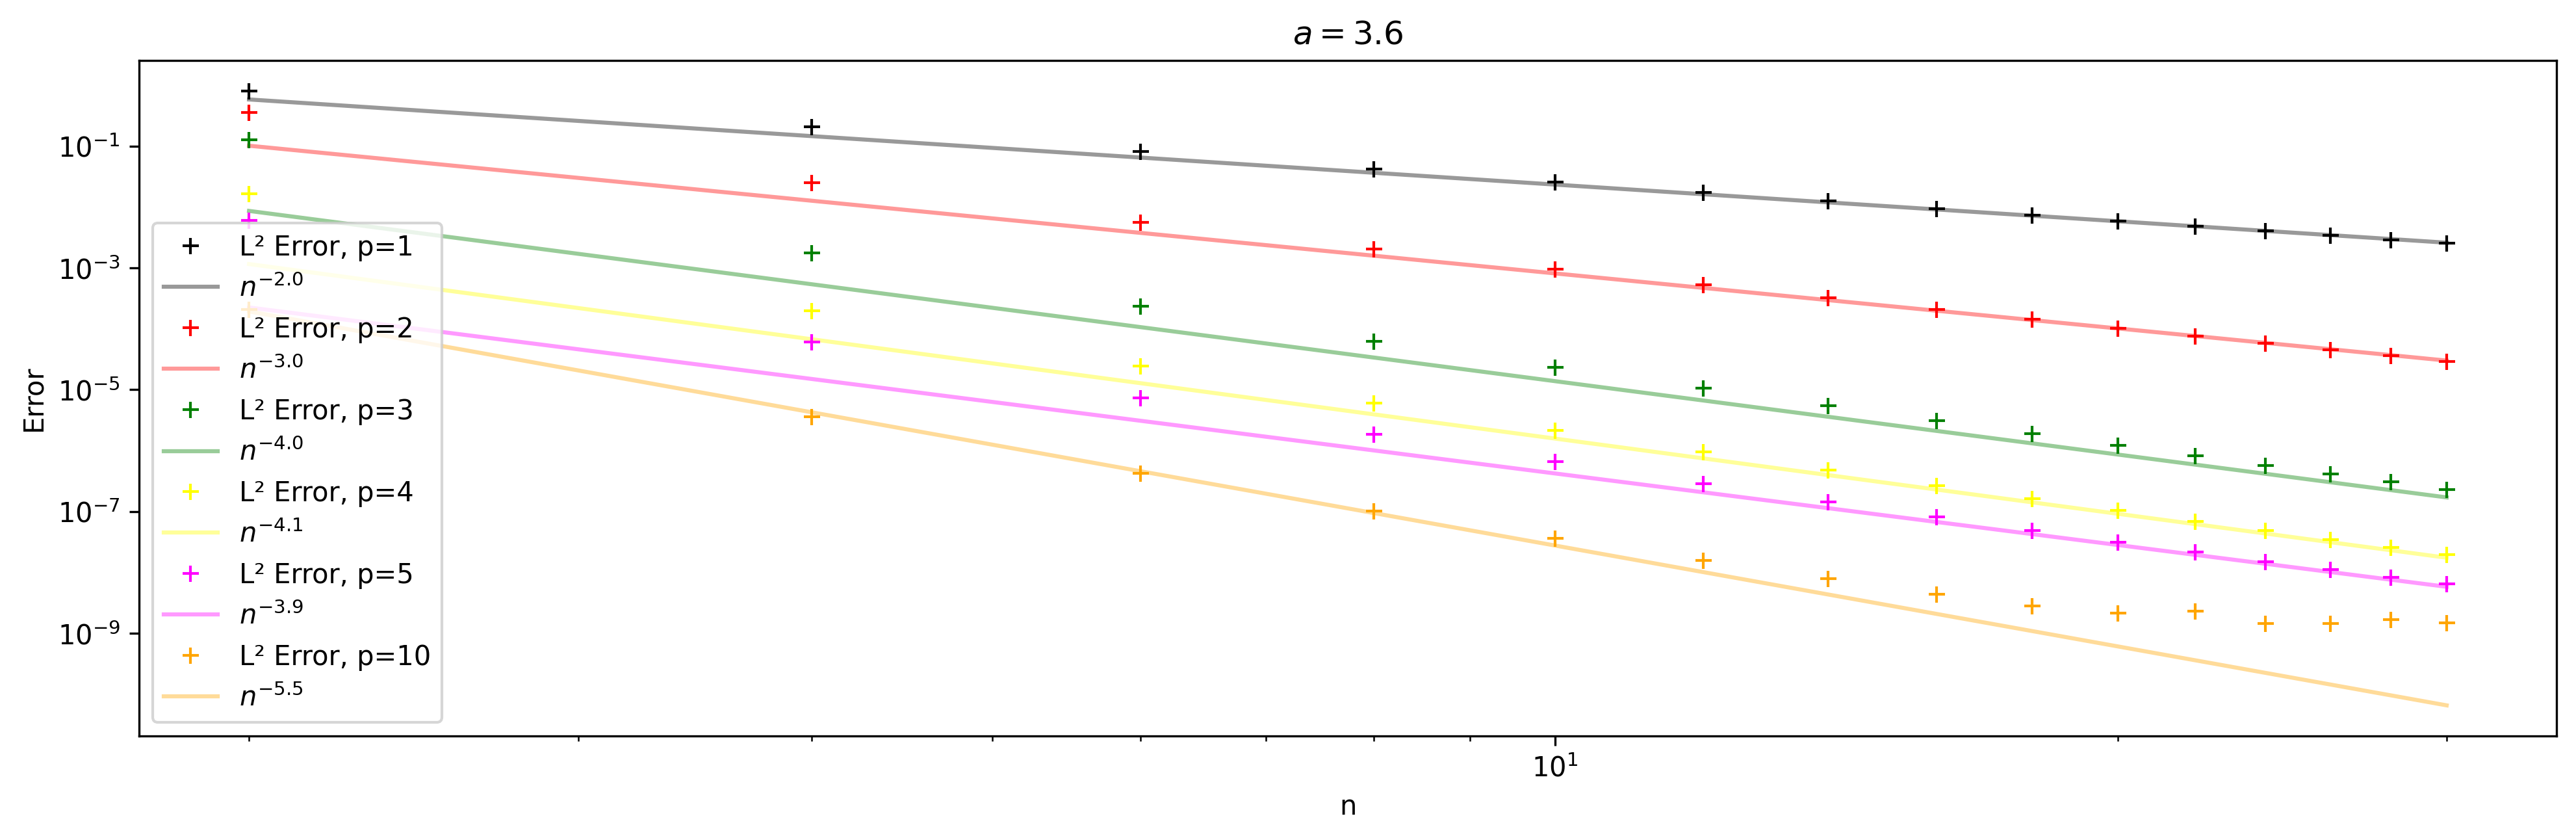
\includegraphics[width=.8\linewidth]{errors_ridge_36_l2}
  \end{subfigure}

  \begin{subfigure}{1\linewidth}
    \centering
    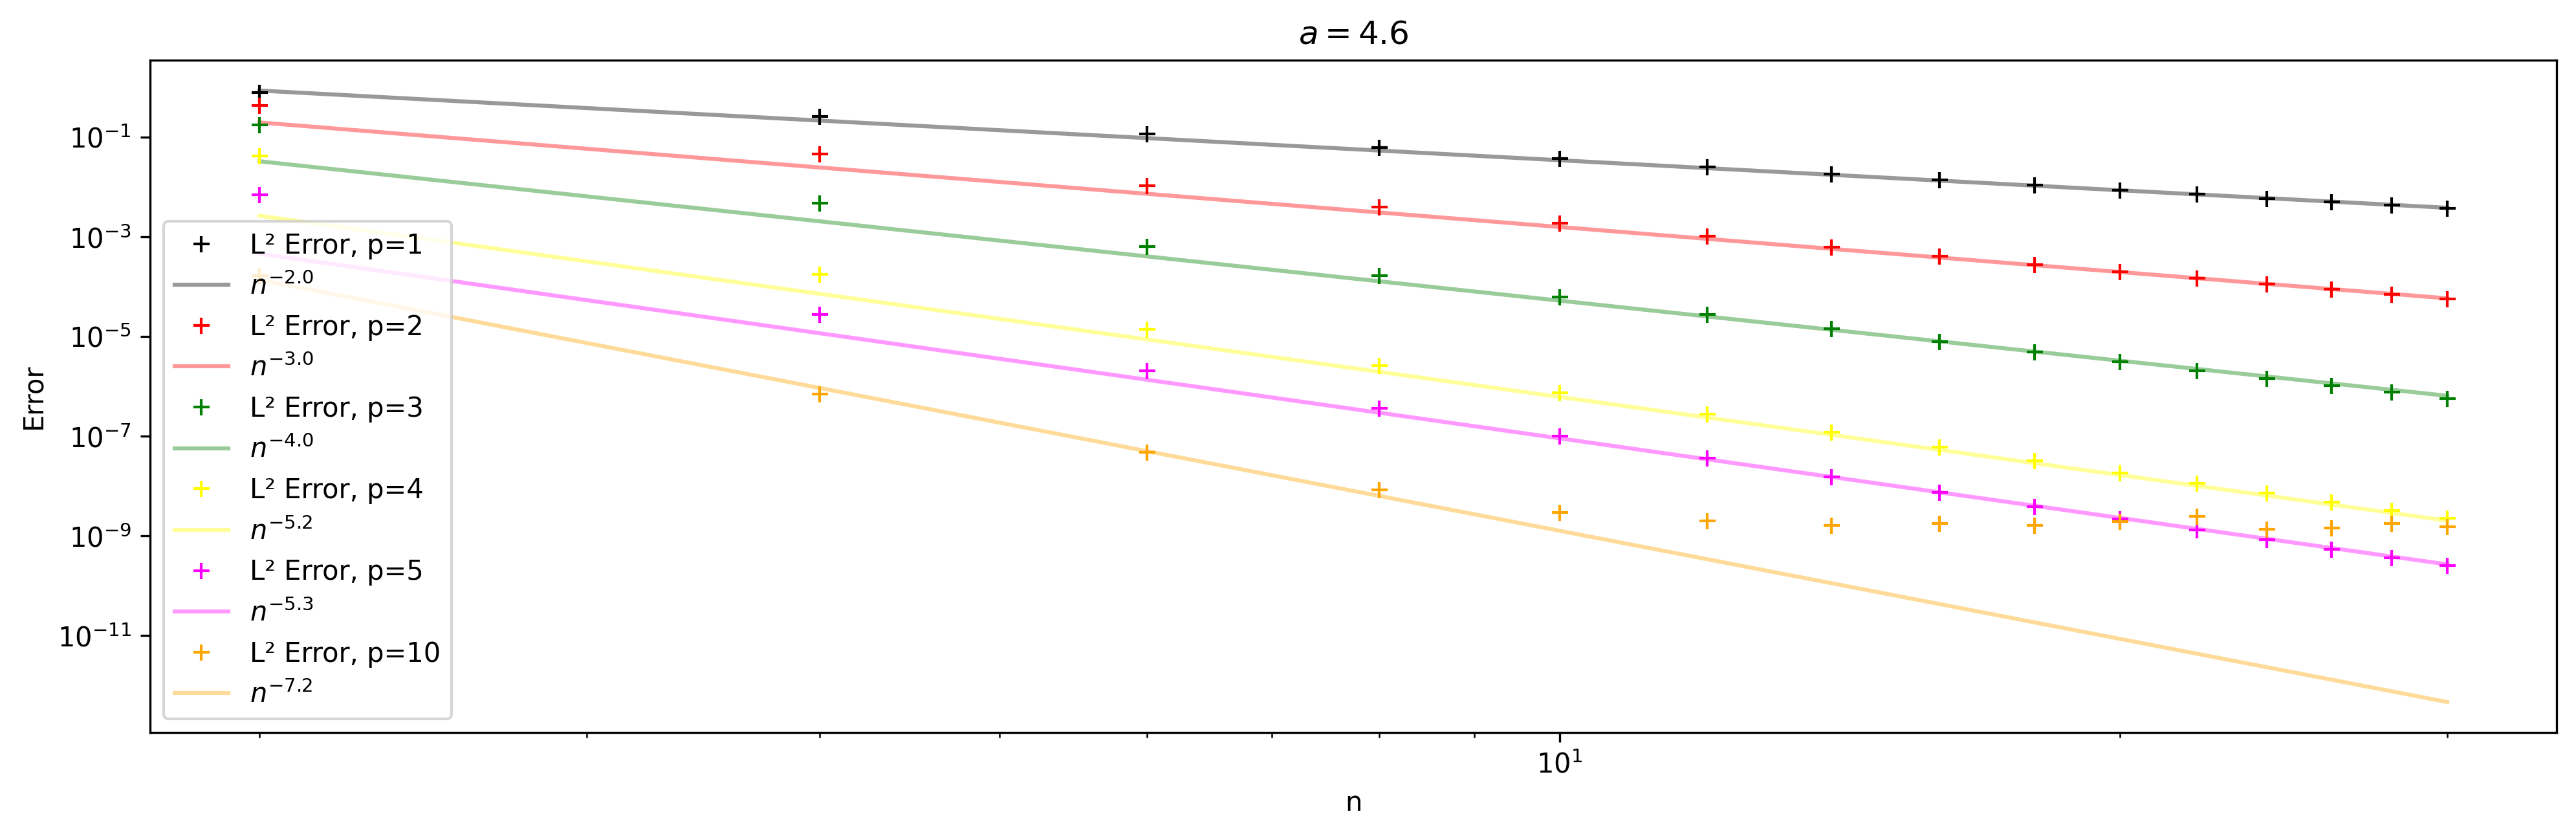
\includegraphics[width=.8\linewidth]{errors_ridge_46_l2}
  \end{subfigure}

  \begin{subfigure}{1\linewidth}
    \centering
    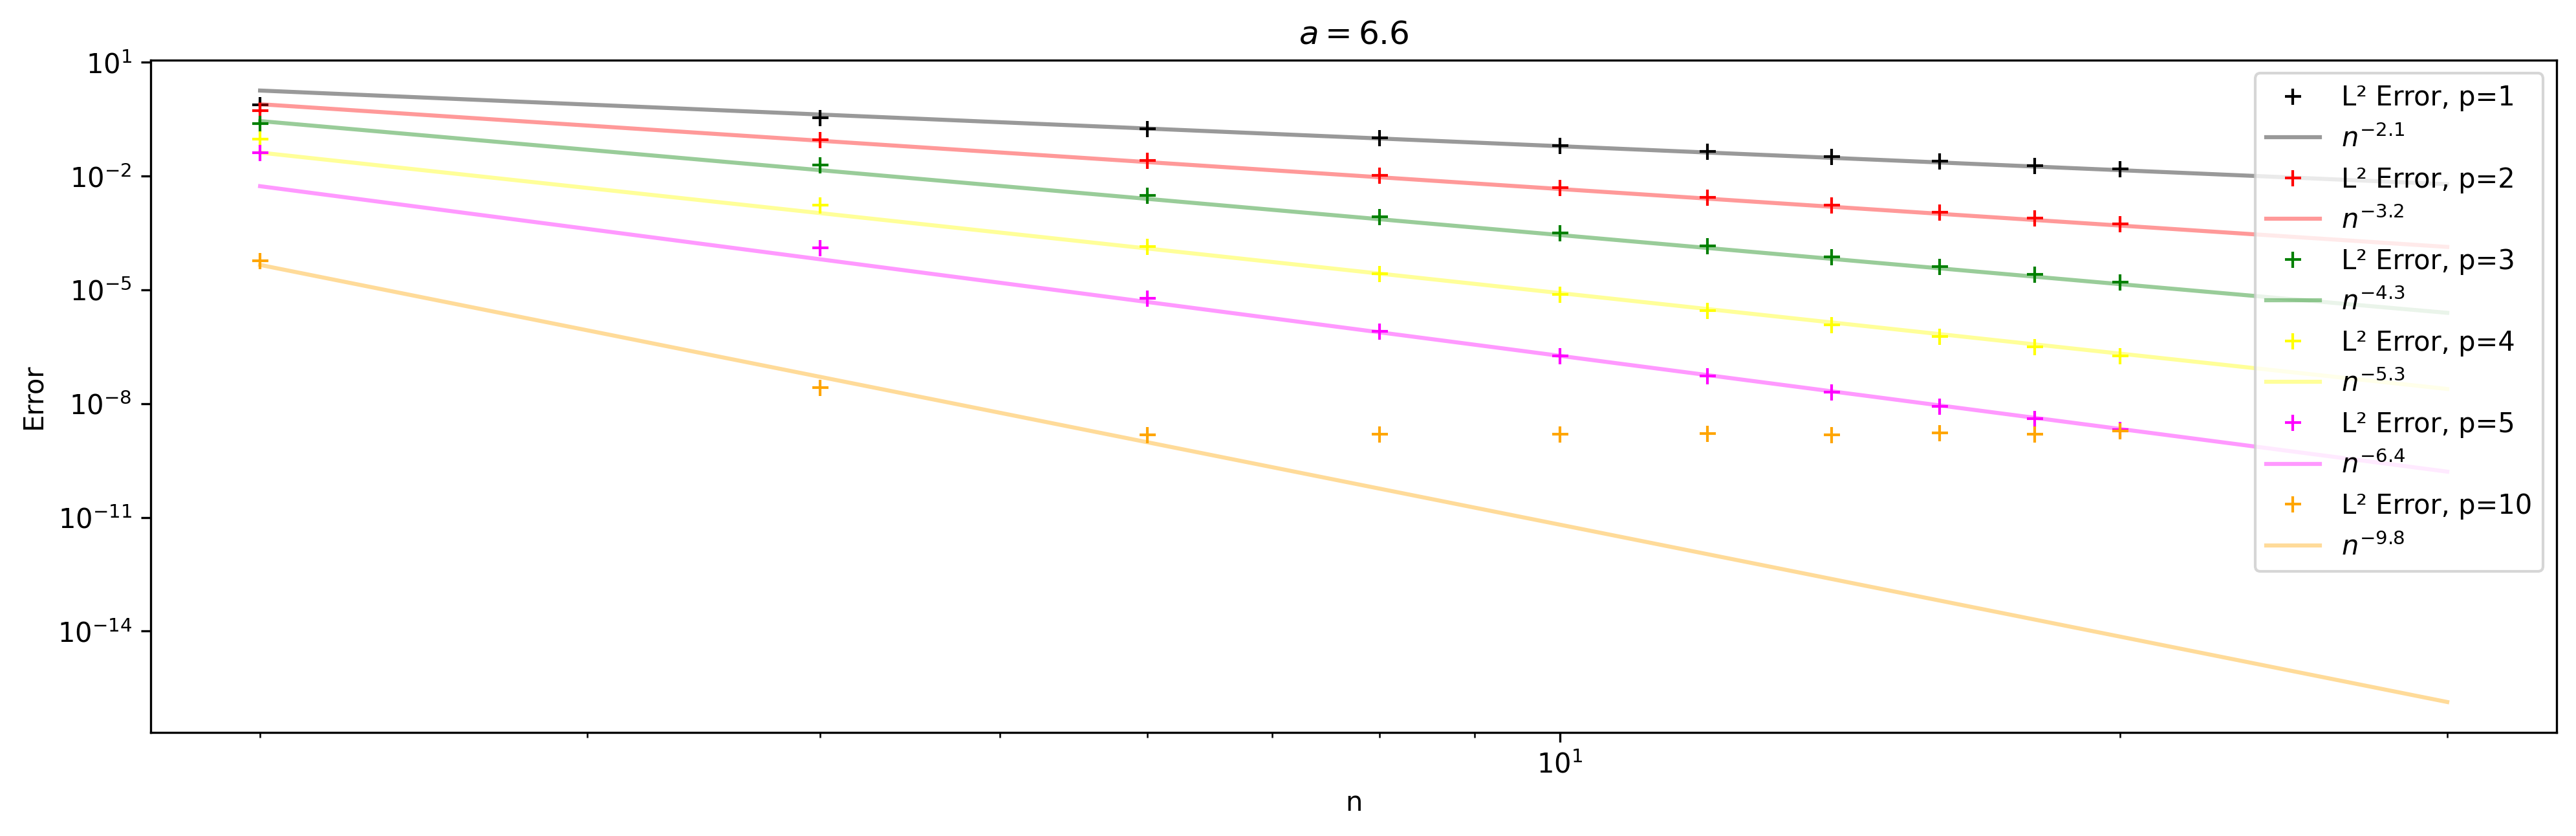
\includegraphics[width=.8\linewidth]{errors_ridge_66_l2}
  \end{subfigure}

  \begin{subfigure}{1\linewidth}
    \centering
    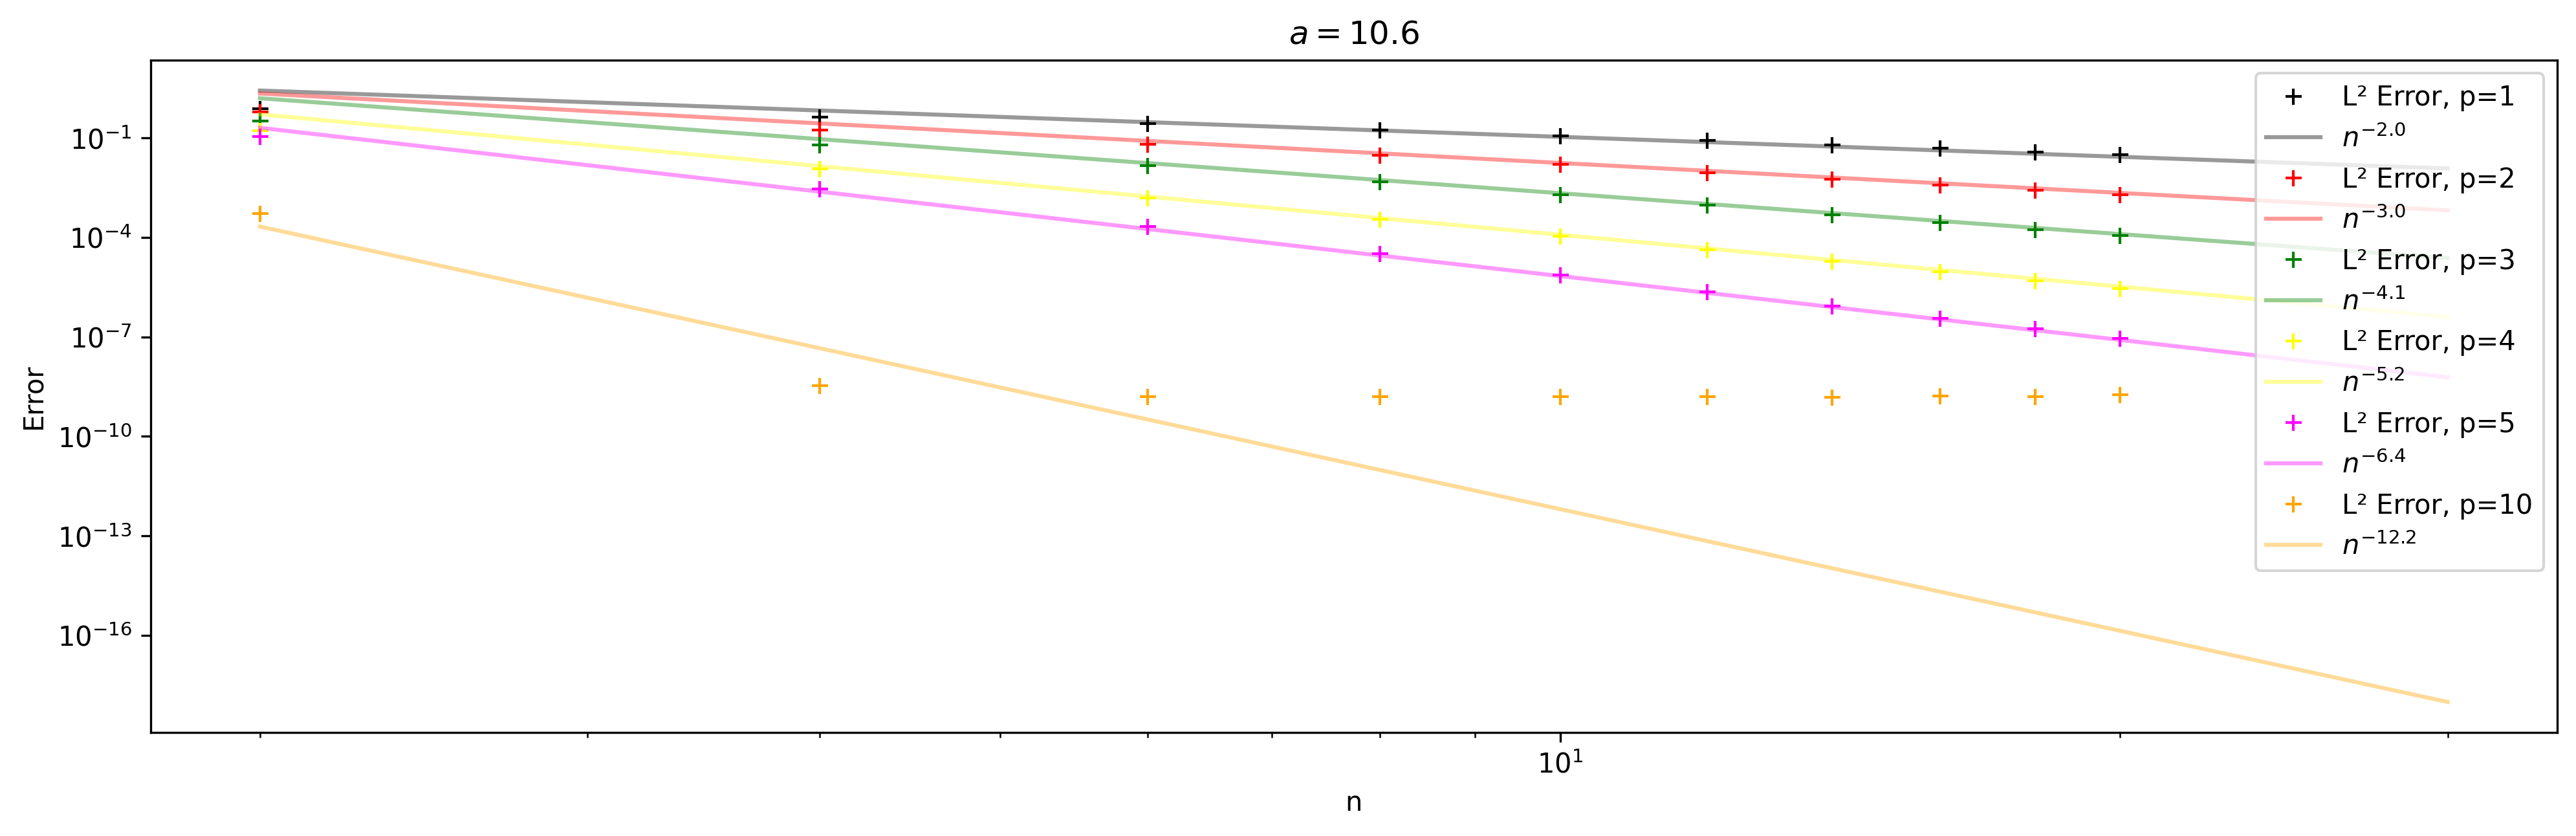
\includegraphics[width=.8\linewidth]{errors_ridge_106_l2}
  \end{subfigure}

  \caption{Convergence With Increasing Smoothness and Higher Order Elements}
  \label{fig:err_ridge_l2}
\end{figure}


\begin{figure}[H]
  \centering
  \begin{subfigure}{1\linewidth}
    \centering
    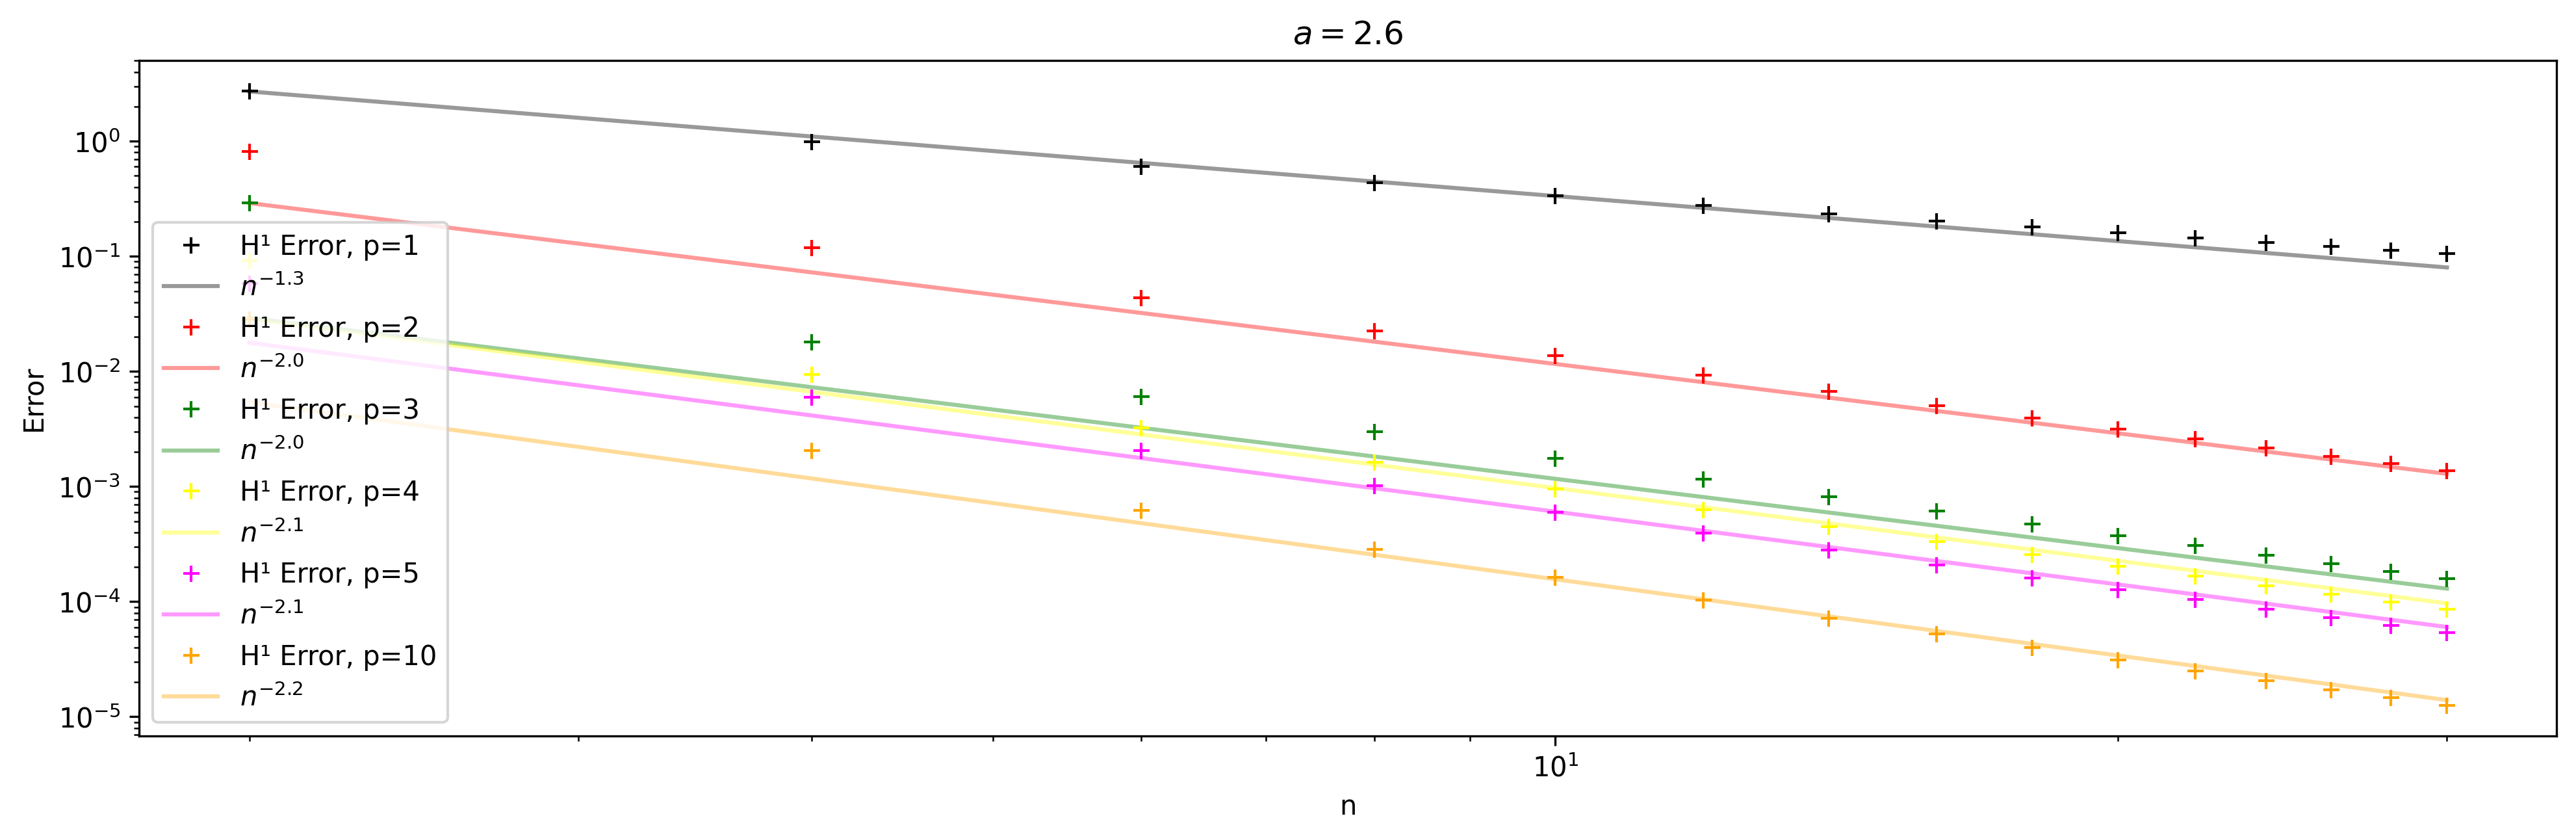
\includegraphics[width=.8\linewidth]{errors_ridge_26_h1}
  \end{subfigure}

  \begin{subfigure}{1\linewidth}
    \centering
    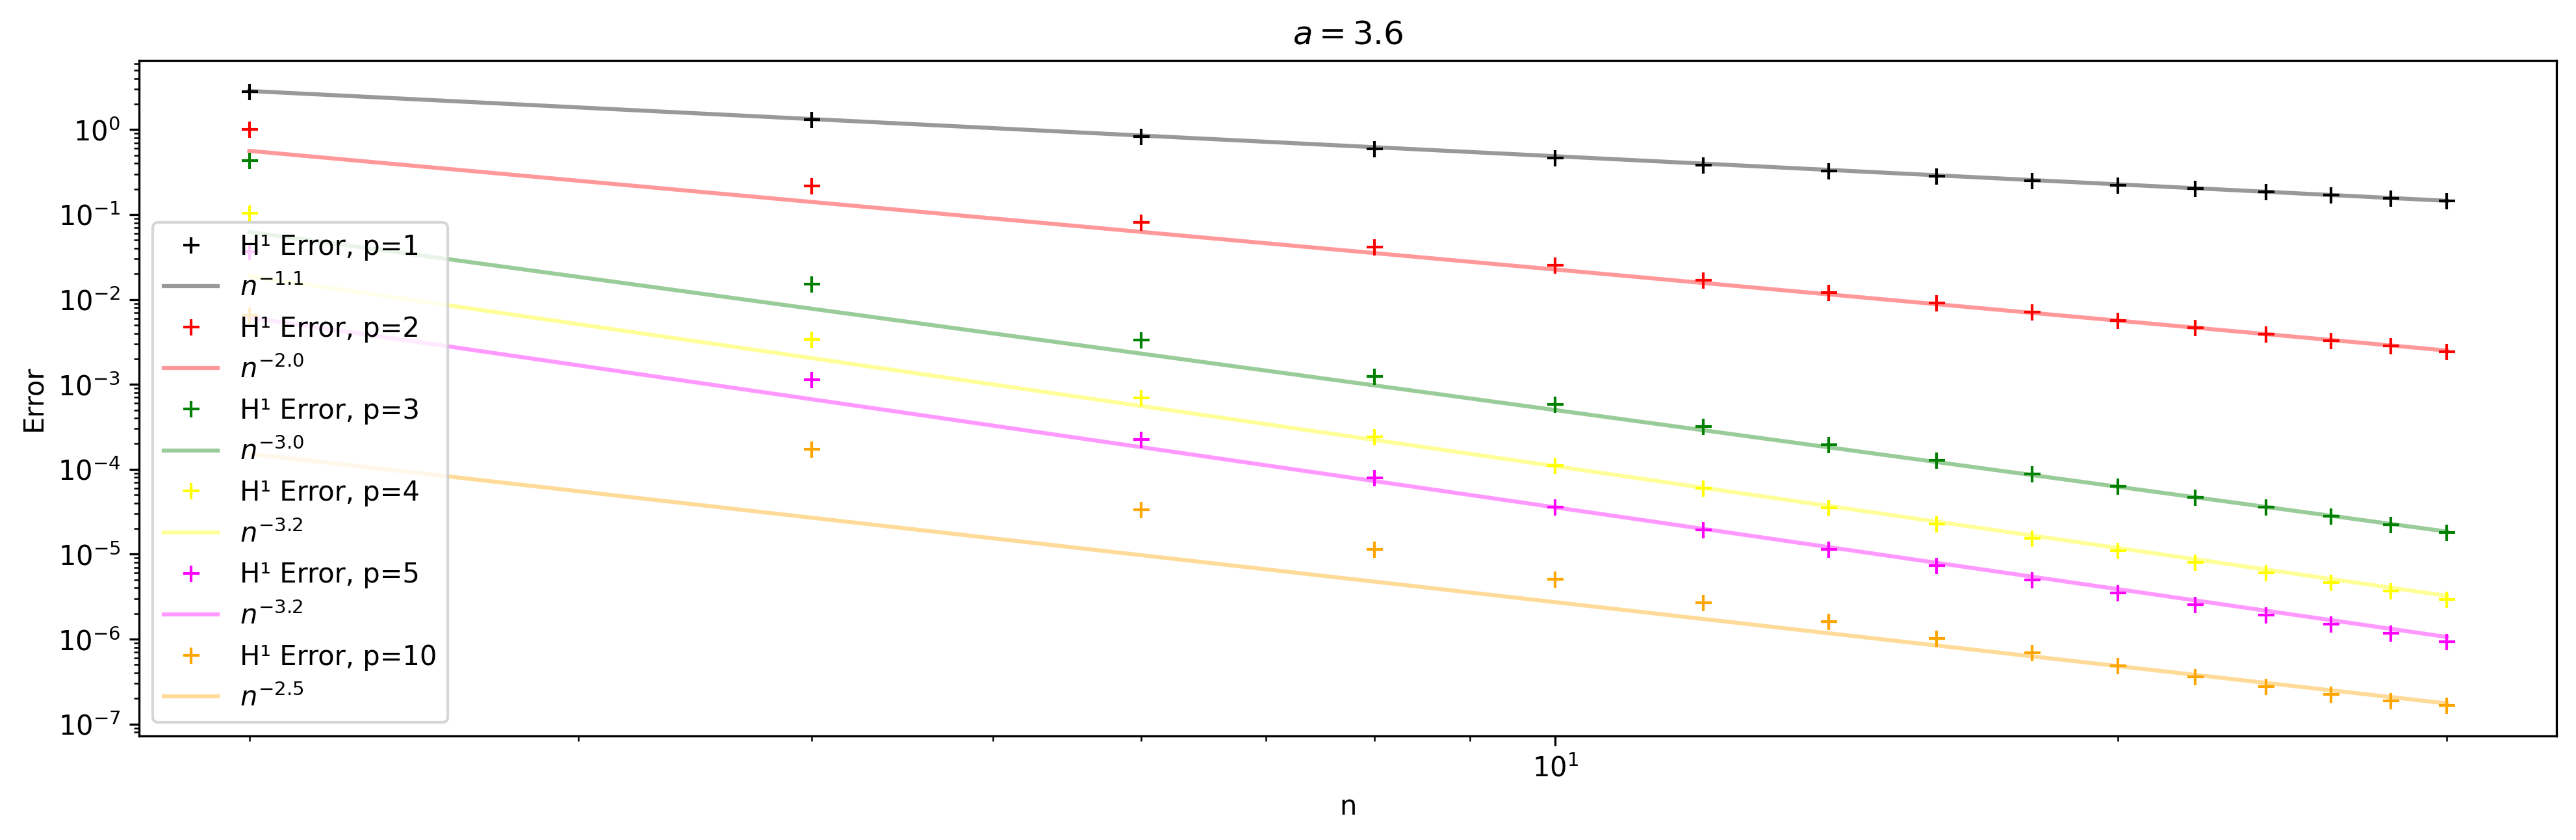
\includegraphics[width=.8\linewidth]{errors_ridge_36_h1}
  \end{subfigure}

  \begin{subfigure}{1\linewidth}
    \centering
    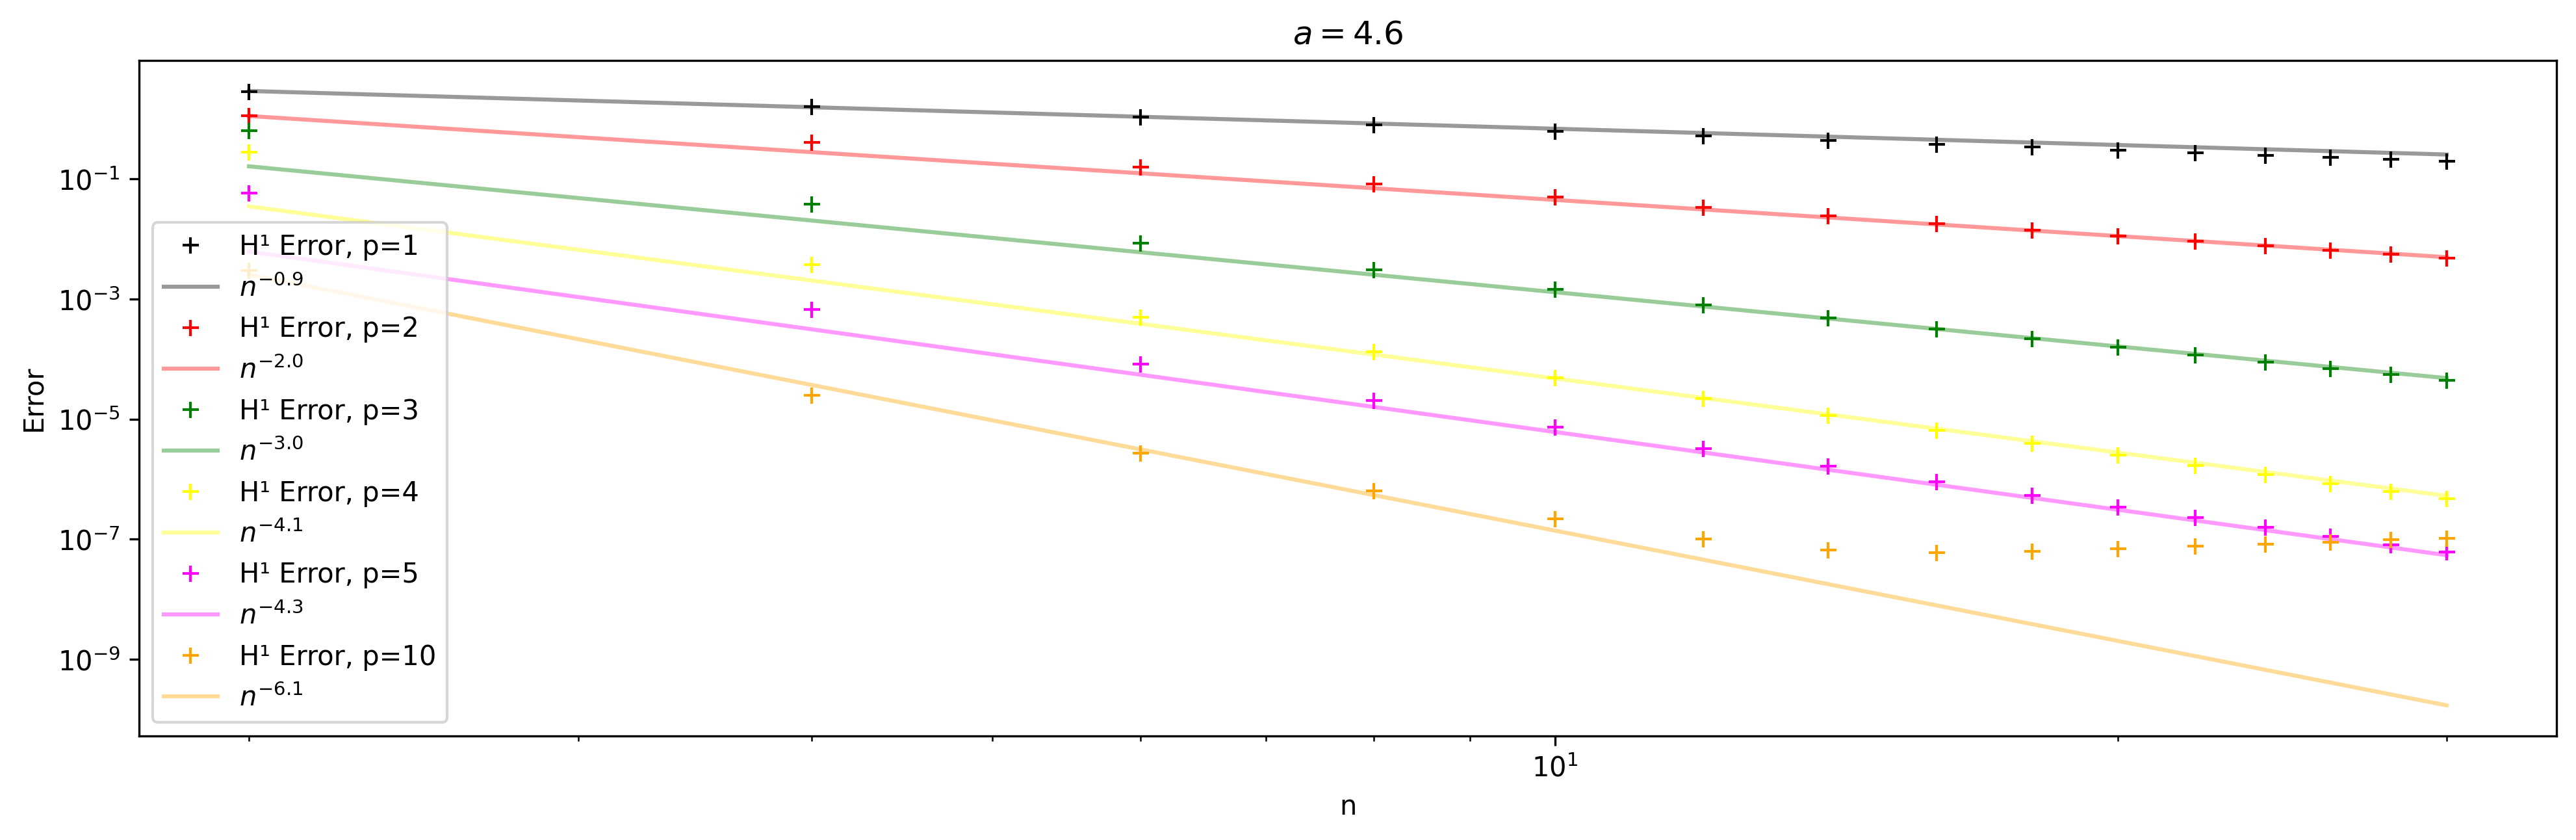
\includegraphics[width=.8\linewidth]{errors_ridge_46_h1}
  \end{subfigure}

  \caption{$H^1$ Semi-Norm Convergence With Increasing Smoothness and Higher Order Elements}
  \label{fig:err_ridge_h1}
\end{figure}


\subsection*{Numerical Challenges}
\subsubsection*{Choice of Basis}
An important step, is the choice of basis functions on the reference element, and how to represent this basis.
In this report, Lagrange elements of varying degree have been used.
These are defined by a set of distinct nodes $X \coloneqq \left\{x_i \in \mathbb{R}^d, i = 1,\cdots, N_p\right\}$ on the reference element.
And the $N_p$ basis functions are defined as:
$$\Phi_i(x_j) = \delta_{i,j}.$$
Where certain restrictions apply on how many nodes must be placed on the boundary.

As the so defined basis does not allow for point evaluation at arbitrary points on the reference element,
those $\Phi_i$ must be explicitly computed.
One now has two choices to make: Where to place the nodes, and in which polynomial basis to represent the $\Phi_i$.
The most obvious and popular choice, which was also used in this work, is using equally spaced nodes and the monomial
basis for $\Phi_i$.

To obtain $\Phi_i$ in the monomial basis, one could compute the inverse of the Vandermonde matrix evaluated at all
nodes $x_i \in X$. Unfortunately, the condition number of the Vandermonde matrix in monomial basis increases rapidly
as seen in \autoref{fig:vandermonde_cond}. For higher order elements this introduces a significant error in the point evaluation
which then propagates to the integration process and thus the solution.
\begin{figure}[H]
  \centering
  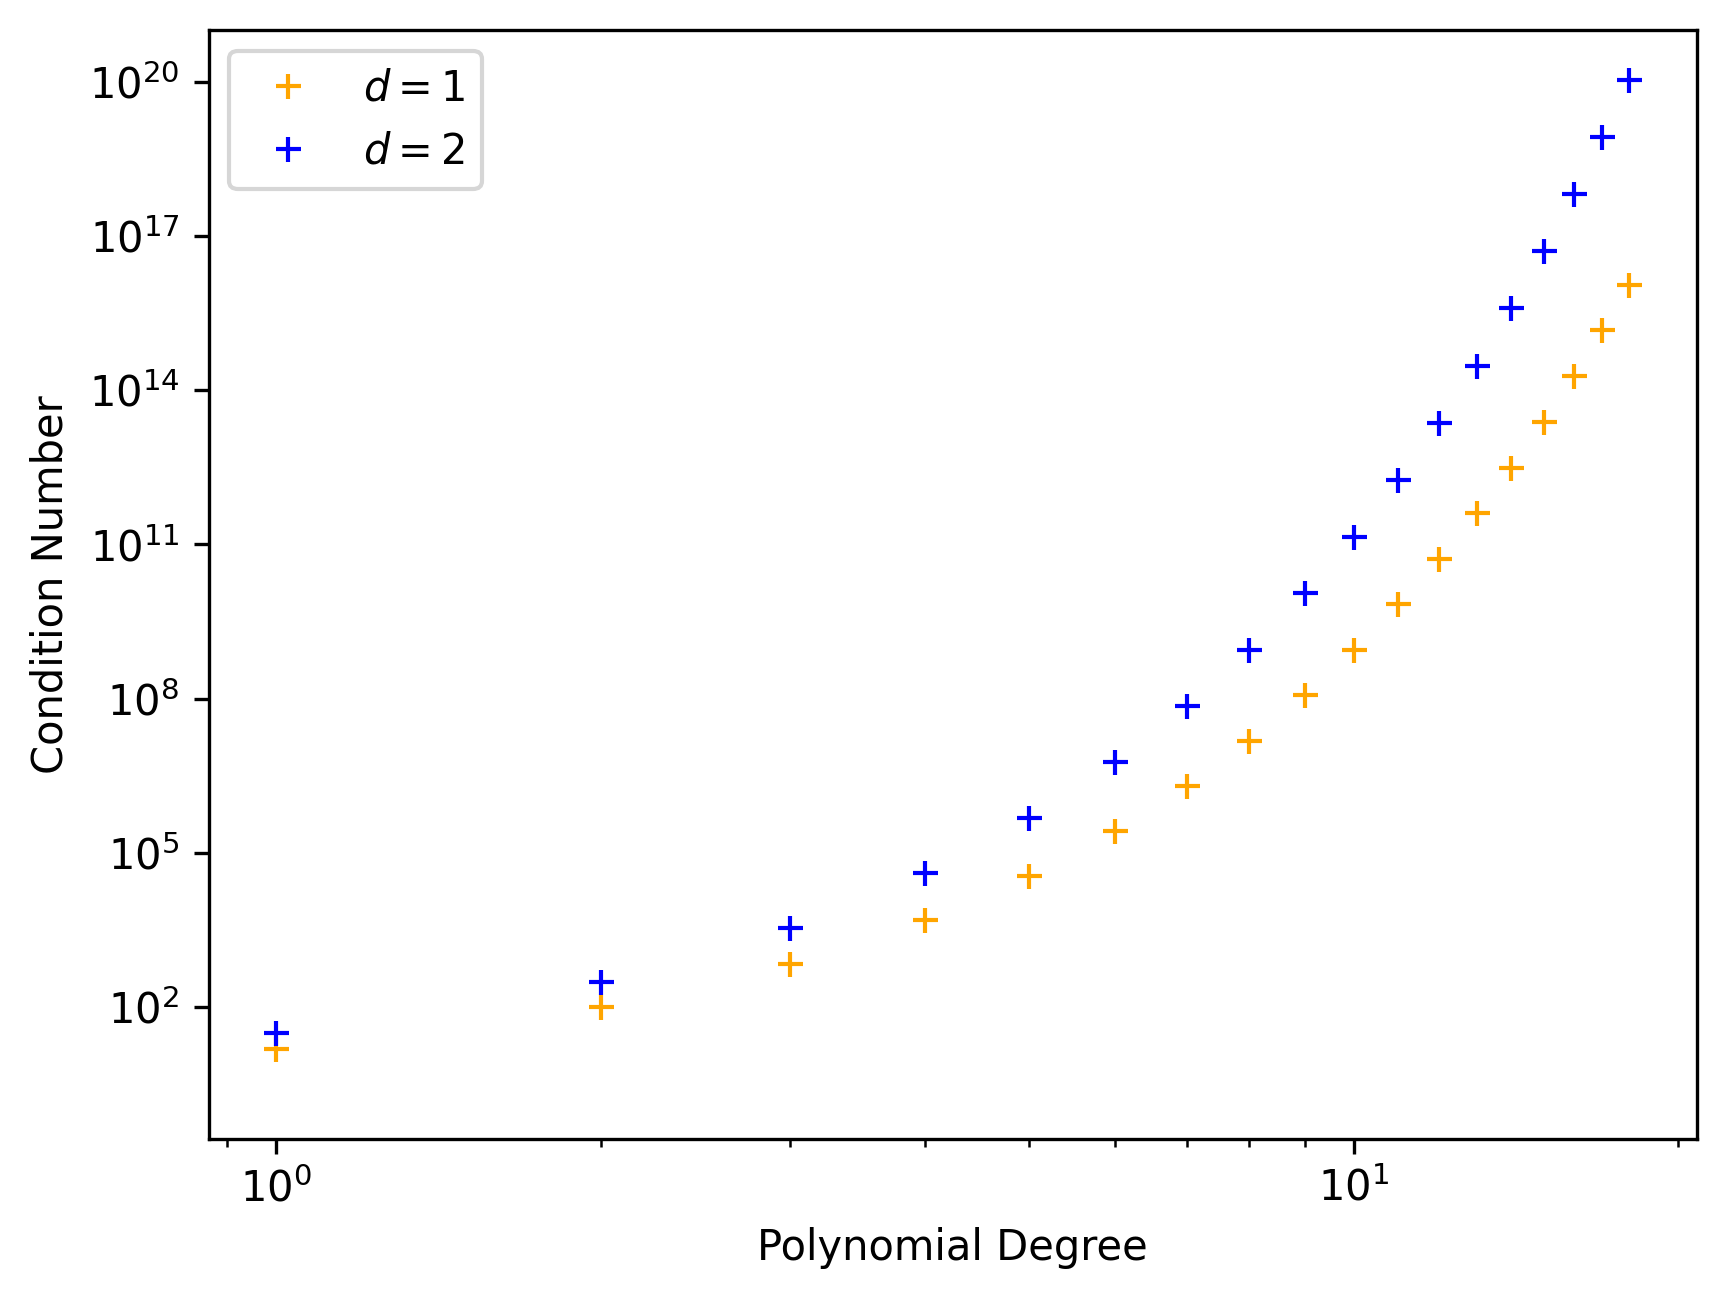
\includegraphics[width=1\linewidth]{vandermonde_cond}
  \caption{Condition Number of Vandermonde Matrix for increasing Polynomial Degree}
  \label{fig:vandermonde_cond}
\end{figure}

\subsubsection*{Singularities}
For weak solutions of \autoref{eq:poisson_weak} to exist, it suffices for the rhs to be square integrable.
Thus, $f$ could potentially be infinite at any countably many points
and point-evaluation of $f$ is not well-defined. However, the integration schemes employed by this
implementation are based on quadrature rules, which rely on point-evaluation. This is remedied by
simply setting all infinite values to $0$, which represents $f$ by a different function from
the same equivalence class, thus not changing the equation. And the numerical experiments suggest, that
this will still lead to convergence to the right solution. As long as only a few points are affected.

Numerical evidence suggests, that elements spanning the singularity give better convergence as seen in
\autoref{fig:oscilation}. Where for odd $n$ vertices are placed on the singularity and for $n$ even they are placed right next to it.
\begin{figure}[H]
  \centering
  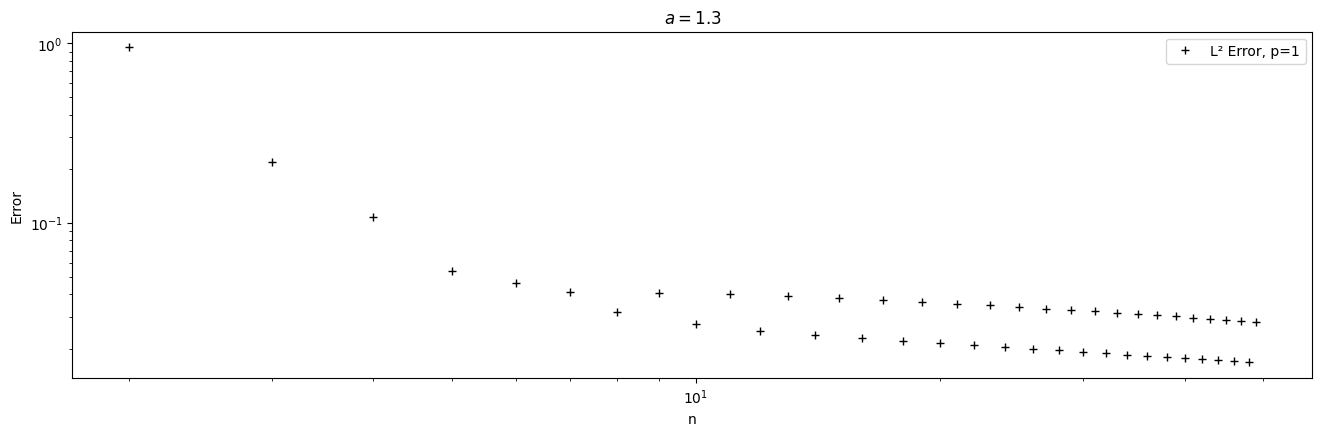
\includegraphics[width=1\linewidth]{oscilation}
  \caption{Oscillating Error depending on meshing of the singularity}
  \label{fig:oscilation}
\end{figure}


\subsubsection*{Submanifolds}
As outlined during the Wednesday lectures, the entire theory is also applicable to immersed manifolds.
As long as they are in some sense well-behaved.
\begin{wrapfigure}{r}{0.5\linewidth}
  \begin{center}
    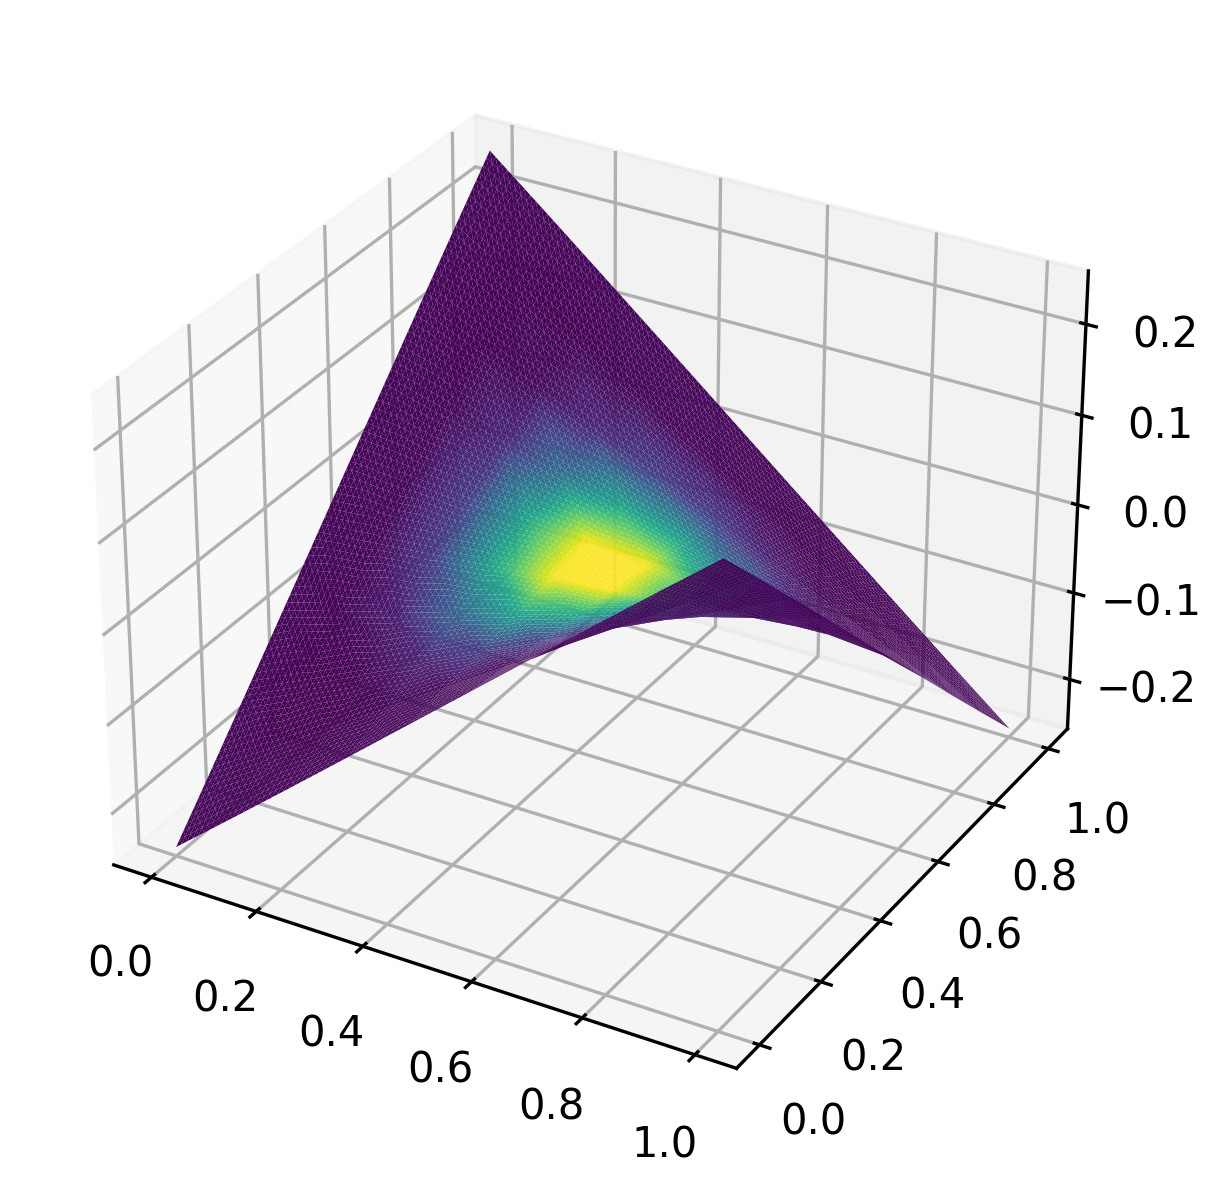
\includegraphics[width=1\linewidth]{submanifold}
    \caption{Solution for Smooth Bump Equation on Submanifold}
  \end{center}
\end{wrapfigure}
The code has been adapted to allow the definition of finite element function spaces on submanifolds.
However, the standard reference elements are not well suited for this, because the curvature of the
submanifold is lost during the triangulation process.

An alternative could be to use non-linear mappings from the reference simplex to the mesh elements.
This complicates the integration process a lot, since the pullbacks to the reference element become
computationally harder to evaluate.

\subsection*{Conclusion}
The Code has been verified by a variety of different problems.
Using different boundary conditions, varying regularity of the force function
and differently structured grids.

The given convergence estimates are exactly met, when expecting solutions clearly falling
into the needed class of functions.
When using borderline cases, where the solution is only just about regular enough,
or just not regular enough any more, the convergence estimates are only exactly met
for a finite amount of steps before the convergence slightly deviates from the expected rate.
As this only happens for edge cases and given the roughness of the estimates, this is not worrying.


To further optimize the implementation, the integration of non-linear transforms of reference elements could be
considered for immersed submanifolds.
To optimize the implementation speed, the global node numbering algorithm should be reconsidered
to optimize the sparsity pattern of the resulting matrix and to optimize memory access.

But as a proof of concept and a tool to investigate convergence rates of higher order elements,
this implementation is well suited.

\end{multicols}
\end{document}
